\documentclass[a4paper,12pt]{report}

% Page setup
\usepackage[utf8]{inputenc} % UTF-8 encoding
\usepackage{geometry} % For customizing page layout
\usepackage{fancyhdr} % For custom headers
\usepackage{setspace} % For line spacing
\usepackage{titlesec} % For custom title formatting
\usepackage{lipsum} % For dummy text
\usepackage{graphicx}
\usepackage{subcaption}
\usepackage{amsmath}
\usepackage{amssymb}


% Page dimensions
\geometry{
    top=2.5cm,
    bottom=2.5cm,
    left=2.5cm,
    right=2.5cm
}

% Line spacing
\onehalfspacing

% Set font to Arial, Tahoma, or Verdana
\renewcommand{\rmdefault}{phv} % Arial font
\renewcommand{\sfdefault}{phv} % Arial sans-serif font

% Title formatting (for custom sections)
\titleformat{\chapter}[block]{\normalfont\LARGE\bfseries}{\thechapter}{1em}{}

% Custom page number settings
\pagestyle{plain} % No header
\pagenumbering{arabic} % Page numbering starting at 1

% Custom section and subsection formatting
\titleformat{\section}[block]{\normalfont\large\bfseries}{\thesection}{1em}{}
\titleformat{\subsection}[block]{\normalfont\normalsize\bfseries}{\thesubsection}{1em}{}

% Remove page numbers on the first four pages
\newcommand{\noPageNum}{\thispagestyle{empty}} % No page number

\begin{document}

% First page (blank)
    \tableofcontents


    \chapter{Introduction}



    \section{Dataset Structure and Initial Challenges}

    The dataset comprises three primary components:


    \begin{itemize}
        \item MepInfo: This dataset contains information on Members of the European Parliament (MEPs).
        \item Votes: This dataset records the votes cast by MEPs on specific pieces of legislation.
        \item Votings: This dataset describes the legislative items that were voted upon.
    \end{itemize}
    \begin{figure}[htb]
        \centering
        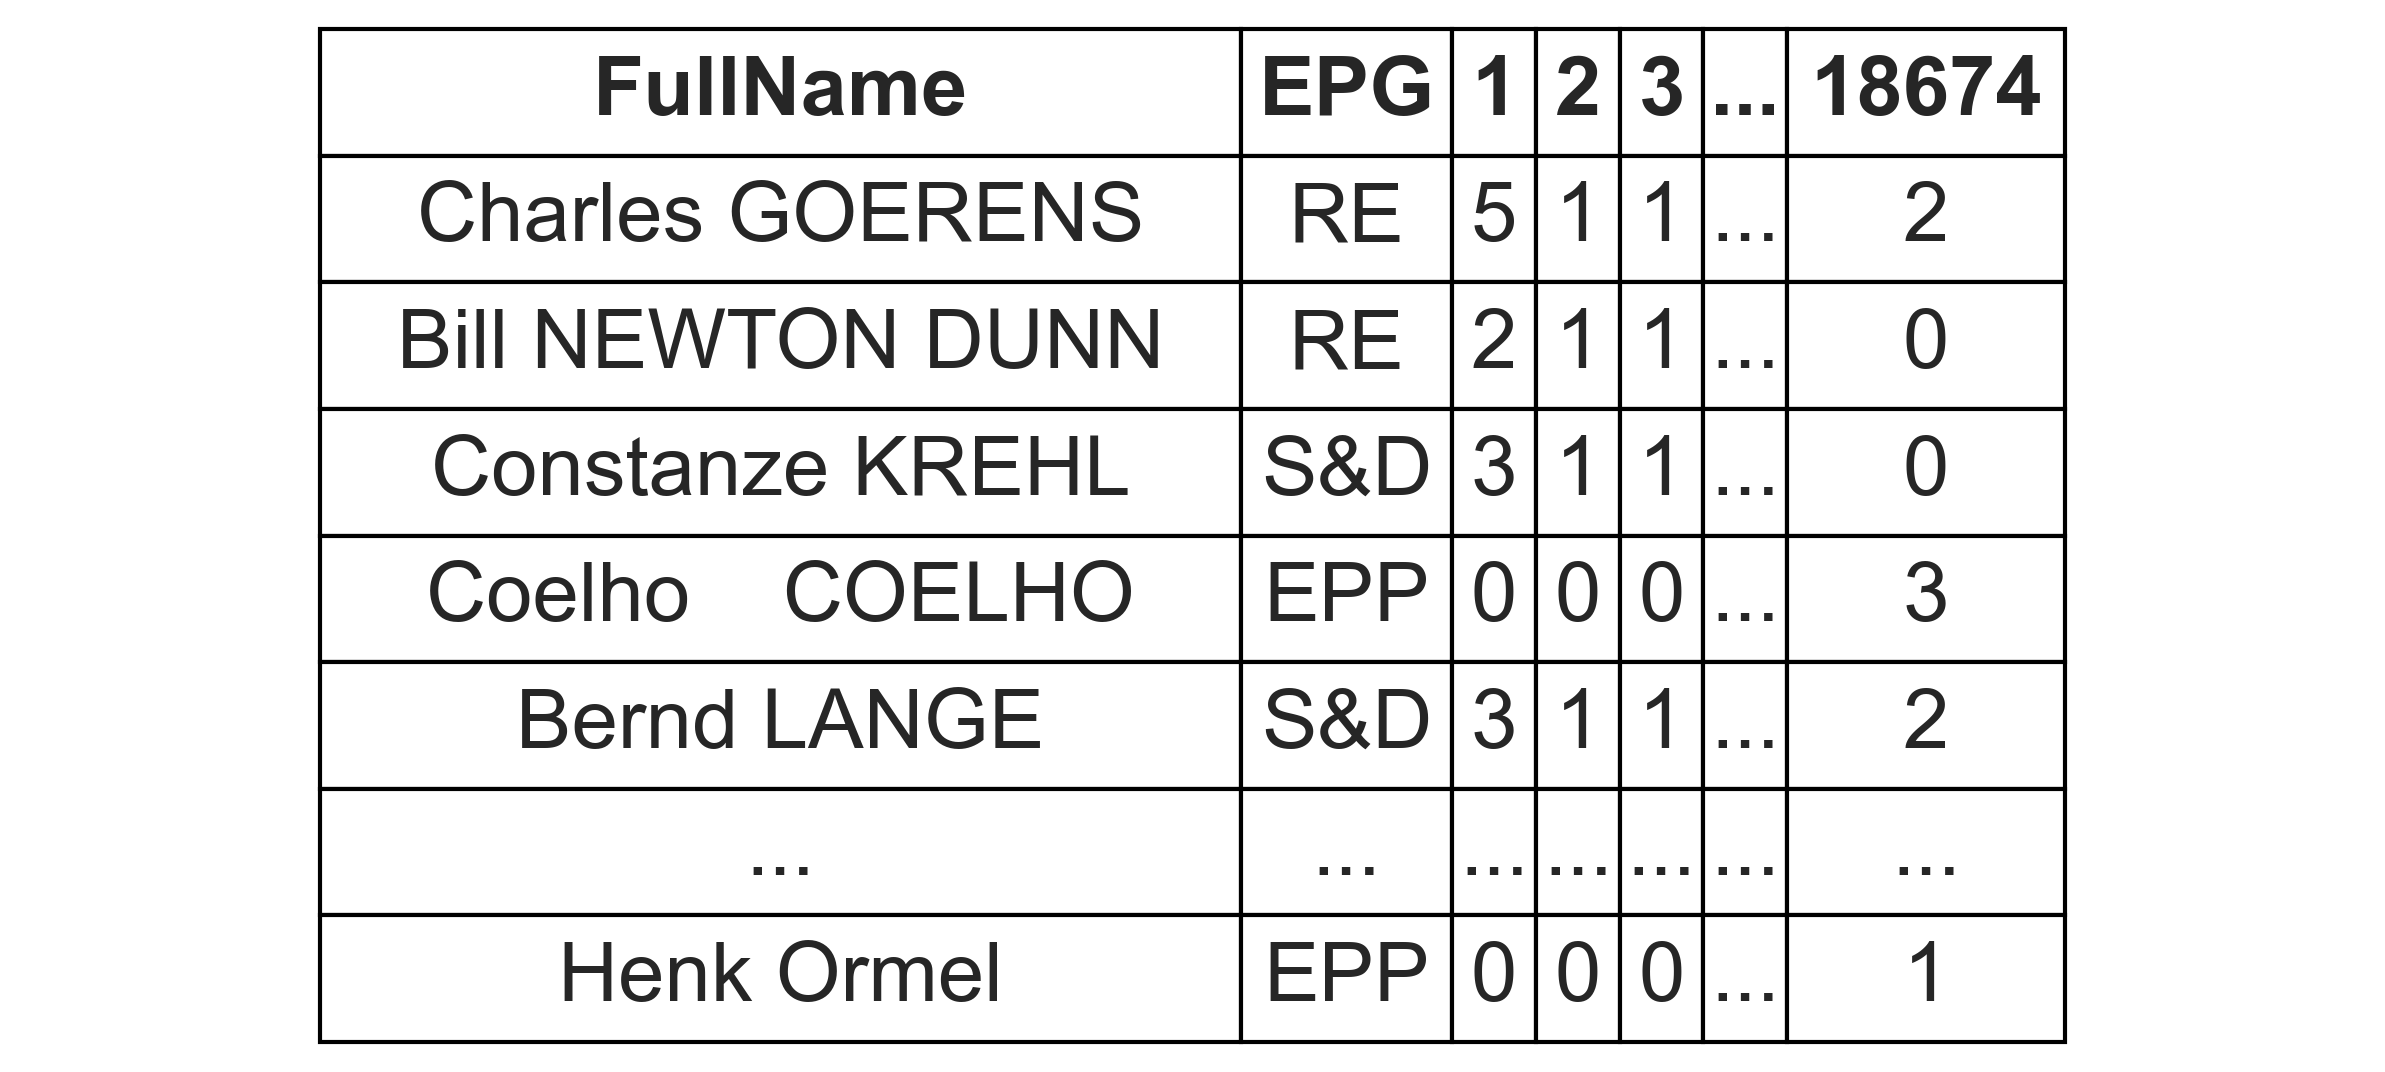
\includegraphics[width=1\textwidth]{Graphs/short_table9}
        \caption{Data from European Parliament 9 formatted for roll-call scaling}
        \label{fig:Structure table}
    \end{figure}

    The Votes dataset alone includes approximately 42,800 roll-calls, with 800-900 MEPs participating in each
    legislature, resulting in an estimated 40 million data points.
    \begin{figure}[htb]
        \centering
        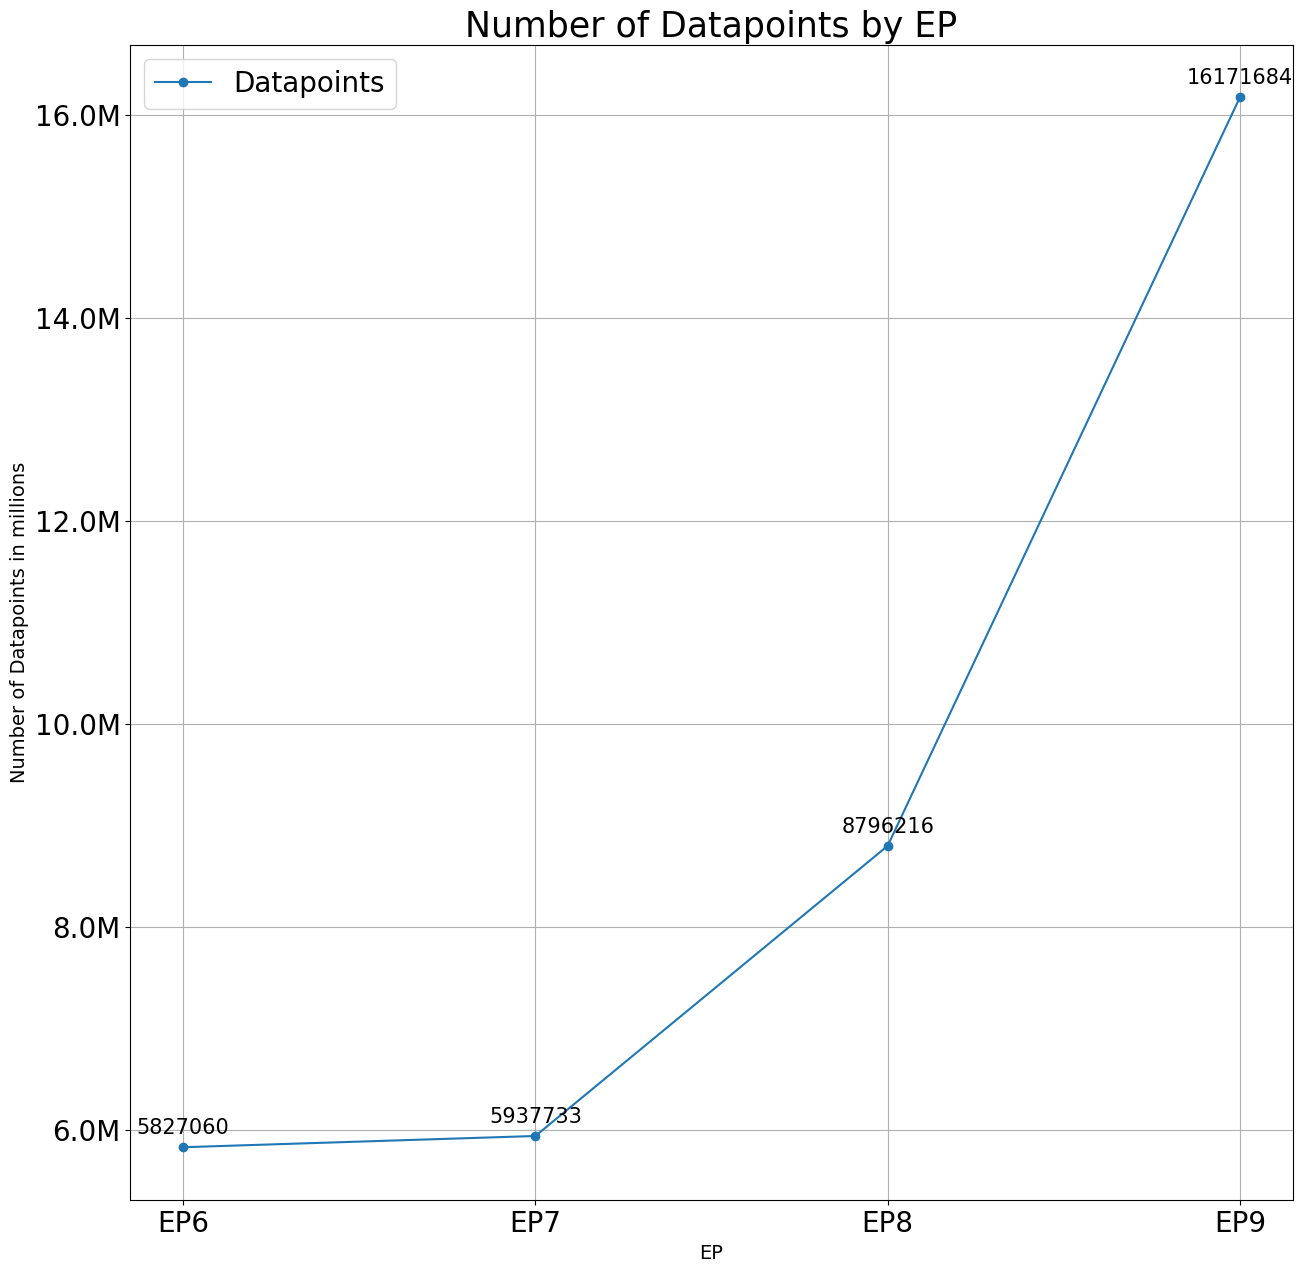
\includegraphics[width=0.8\textwidth]{Graphs/Datapoints}
        \caption{Number of datapoints by European Parliament (EP)}
        \label{fig:Datapoint graph}
    \end{figure}

    The size of the dataset makes for a serious practical challenge in terms of storage and processing, not to
    mention the problems with formatting and integrity of the dataset.
    Upon initial examination, several issues
    with the
    legacy data became apparent:

    \begin{itemize}
        \item
        Missing Variables: The MepInfo dataset lacked several critical variables, including gender and age.
        \item
        Inconsistencies and Missing Observations: Some variables such as Party affiliation and European
        Parliament Group
        (EPG) affiliation were either inconsistent or incomplete.
        \item
        Non-Standard MEP IDs in EP7: MEP IDs in the 7th Parliament did not conform to the standard European
        Parliament
        API format.
        Instead of unique identifiers, incrementing integers were used.
        \item
        Naming Conventions: MEP names and surnames were not consistent with those in the European
        Parliament API.
        \item
        Incorrect and Inconsistent Encoding of Missing Data: Missing data was inconsistently encoded, with
        symbols like
        - or .
        being used in place of null values.
        \item
        Inconsistent Datetime Formatting: Datetime values were formatted inconsistently across the dataset,
        making them
        difficult to import and process.
        \item
        Non-Standard Encoding of Binary Categorical Variables: For example, the binary categorical variable
        `Vote'
        which indicates whether a vote passed or not, was encoded as + and - instead of the standard 1/0 used
        elsewhere
        in the dataset.
    \end{itemize}
    Additionally, the dataset was stored in a long format tailored to the specific analytical requirements of
    the
    original VoteWatch team.
    While this structure was suited to their immediate needs, it posed challenges for
    long-term
    usability, warehousing, and broader analytical purposes.


    \chapter{Data Cleaning Process}\label{ch:data-cleaning-process}


    \section{Supplementing and Correcting the MepInfo Dataset}
    \label{sec:supplementing-and-correcting-the-mepinfo-dataset}


    The initial challenge involved supplementing and correcting the MepInfo dataset to fill in missing variables
    and
    rectify inconsistencies.
    The European Parliament's API played a crucial role in this process. An API
    (Application
    Programming Interface) is a set of defined rules and protocols that allows one software application to
    interact with
    another.
    In the context of scraping data, an API serves as an intermediary that lets users request and
    retrieve
    specific data from a website or service in a structured format, typically JSON or XML, without the need to
    manually
    scrape the HTML content of a webpage.
    Using an API for data scraping is often more efficient and reliable than traditional web scraping, as it
    provides
    direct access to the desired data, reducing the risk of encountering issues like changes in webpage
    structure or
    content restrictions.
    This API provides endpoints, such as `/meps`, which return JSON data containing basic
    MEP
    information, including a unique identifier (MepId).
    By utilizing this API, we were able to standardize the
    names and
    identifiers of MEPs across most legislatures by joining the tables by MepId.

    However, the 7th Parliament (EP7) presented a unique challenge.
    The MEP IDs in this legislature were not
    unique and
    were instead represented by incrementing integers.
    To address this issue, we employed the `fuzzywuzzy`
    Python
    package, which uses the Levenshtein distance algorithm to calculate the similarity between strings. This
    allowed for
    making an approximate match of full names from the original dataset to the `sortLabel` field in the API
    data,
    providing the correct MEP IDs. Manual verification and correction of edge cases were necessary to ensure
    accuracy.

    Despite these efforts, some data remained incomplete, particularly regarding MEPs who changed parties or
    EPGs during
    their tenure, as well as demographic data such as gender and birth dates. These gaps required further manual
    supplementation, which is discussed in detail in the Automation section.


    \section{Addressing Inconsistencies in the Votings Dataset}
    \label{sec:addressing-inconsistencies-in-the-votings-dataset}

    The Votings dataset required significant work to address encoding inconsistencies and improperly formatted
    datetime
    values.
    The first issue was relatively easy to reconcile using renaming dictionaries to replace inconsistent
    encodings in some variables.

    However, the latter issue proved particularly problematic due to the original data being gathered in Excel.
    Manual
    formatting likely led to inconsistent datetime values formatting.
    To standardize the format, manual
    correction of
    the dates was necessary before applying the Pandas `to datetime` function.

    This step ensured that the datetime values were correctly parsed and made the data suitable for further
    analysis.
    Once the initial cleaning was complete, a new challenge arose.
    In 2022, the original VoteWatch team altered
    their
    data gathering methodology.
    Consequently, data from Parliament 9, covering the period until 2022, was
    consistent
    with earlier practices.
    However, data collected from 2022 to March 2024 exhibited several discrepancies. The
    order
    of VoteIds had changed, some columns particularly those in the Votings dataset were missing, and special
    characters
    were corrupted due to encoding issues.
    To resolve these issues, we employed a multistep approach.
    First, we used a dictionary to replace the corrupted characters systematically.
    Next, we reverse-engineered the missing Votings columns (such as finalVote, a binary
    variable of whether a vote is a last one in a section) from the available data.
    Despite the complexity of these tasks,
    they were necessary to restore the integrity and consistency of the dataset, ensuring that it could
    be
    seamlessly integrated with the existing data from earlier legislative periods.


    \section{Data Restructuring for Long-Term Usability}\label{sec:data-restructuring-for-long-term-usability}

    With the Votes and MepInfo datasets cleaned and supplemented, the next step was to restructure the data into
    a
    format suitable for long-term storage, analysis, and future updates.
    The data was initially stored in a long
    format,
    where each row represented an observation, and columns represented variables.
    To facilitate analysis, we
    separated
    the MepInfo and Votes datasets into distinct tables:
    \begin{itemize}
        \item
        MepInfo table contained all variables describing the MEPs, with `MepId` serving as the primary key.
        \item
        The Votes table used a composite primary key consisting of `MepId` and `VoteId`, a unique identifier for
        each
        voting event.
        This table also included a column encoding the MEPs' votes.
    \end{itemize}

    These tables were linked by primary keys, allowing for efficient querying and data retrieval. For example,
    using the
    `MepId`, one could easily retrieve all votes cast by a particular MEP, and by further referencing the
    `VoteId`,
    additional context from the Votings table could be added.

    To support the development of the European Parliament Vote Monitor website, the voting data was additionally
    exported in `.csv` format, organized by month and year. This format was chosen to optimize data storage and
    accessibility, ensuring that the data could be easily updated and queried. Additionally, for specialized
    analytical
    purposes, the Votes data was also retained in its original matrix format, now enhanced with the newly
    cleaned and
    supplemented variables.


    \chapter{Automation of Data Gathering}\label{ch:automation-of-data-gathering}


    \section{Overview of the European Parliament API}\label{sec:overview-of-the-european-parliament-api}

    With the historical data cleaned and restructured, the next phase of the project focused on automating the
    future
    data gathering process. Consistency and reliability were paramount in this process. The previous VoteWatch
    team
    relied on scraping XML files from the human-readable official minutes on the European Parliament's website,
    coupled
    with downloading MepInfo from the API. This approach was fraught with challenges, including the potential
    for
    inconsistencies in the scraped data, lack of unique identifiers, and the inherent unreliability of scraping
    human-readable content.

    To address these issues, we transitioned to using the European Parliament's open API, which provides direct
    access
    to structured data in a reliable and consistent manner. The API is publicly accessible, meaning no API key
    is
    required, and it allows users to specify parameters in the URI to retrieve data from various endpoints.


    \section{MepInfo Data Collection Automation}\label{sec:mepinfo-data-collection-automation}
    The `/meps` endpoint of the API, which provides a list of MEPs along with their unique identifiers, was the
    starting
    point for automating the MepInfo data collection. However, the data returned by this endpoint was not
    exhaustive. To
    gather more detailed information such as MEPs' gender, age, and political affiliations additional API calls
    were
    required to other endpoints within the `meps` group.

    For example, to retrieve data on MEPs' party memberships and affiliations with European Political Groups
    (EPGs) and
    National Parties, separate API calls were made specifying the MepId . The resulting data was then filtered
    and joined
    with the MepInfo dataset to create a comprehensive record of each MEP s political affiliations and
    demographic
    information.

    One key challenge in this process was optimizing the API calls to minimize the load on the server. Each MEP
    required
    an individual API call to gather detailed data, which could result in approximately 850 GET requests per
    scraping
    session. To mitigate this, the metadata was included in the same call to avoid the need for additional
    requests.

    Another consideration was the use of non-human-readable IDs for certain values, such as the organization
    field,
    which required further API calls to retrieve the corresponding labels from the `corporate-bodies` endpoint.
    For
    example org/1537 was an identifier for GUE/NGL EU Political Group. These labels were essential for
    understanding the
    data and were subsequently joined with the MEPs' political affiliation data.


    \section{Votings Data Collection Automation}\label{sec:votings-data-collection-automation}

    The `meetings` endpoint of the API was utilized to automate the collection of data on plenary sessions and
    the
    decisions made during these sessions. An initial API call returned a list of all plenary sessions that took
    place in
    a given year. This list was then filtered by month to identify the specific sessions relevant to the current
    data
    collection period.

    For each identified session, further API calls were made to retrieve detailed voting data, such as the votes
    cast by
    each individual member and all of the supplementary data that was previously found in the Votings database.
    This
    data was then merged with the previously gathered MepInfo and Votes data, ensuring that all relevant
    information was
    captured and linked across the collection.

    In order to automatically gather the data in the future, working with a Bocconi IT Department team, we
    created a
    cloud-based solution that is deployed and triggers every month, gathering and exporting the data to the .csv
    format,
    as well as to a relational SQL database.


    \chapter{Ideal Points Estimation - Overview of Current Methods}
    \label{ch:ideal-points-estimation---overview-of-current-methods}
    One of the most prominent uses of voting data in political science research is estimating ideal points of
    legislators on the ideological plane. The early revolutional work of Poole and Rosenthal (1985) set the
    precedent for using those types of algorithms - specifically NOMINATE - Nominal Three Step Estimation on
    larger datasets than previously possible. Ever since, ideal points estimation was developed more and more,
    with improved versions of the original algorithm (such as D-NOMINATE, and later W-NOMINATE), to extending
    its implementation beyond the original usecase (scaling the US parliament), analysing the European
    Parliament and various national parliaments. The European parliament specifically has had a great deal of
    coverage using the W-NOMINATE method, which has been the standard for the past 20 years.


    \section{W-NOMINATE}

    \subsection{Algorithm}

    W-NOMINATE (Weighted NOMINATE) - an improved version of NOMINATE, used for estimating legislator's
    ideal points relying on their roll-call voting records. The underlying model of NOMINATE, and by
    extension, W-NOMINATE is a spatial voting model, where legislators and the policies are represented
    in a multidimensional space. In this implementation, a legislator has an ideal point in this space,
    that represents their ideology and policy preference, and each vote is a set of two alternative
    points - one when the policy is implemented (the vote passes), and another when the policy is
    rejected (the vote fails). W-NOMINATE assumes that legislators vote for an outcome that is closest
    to their ideal point, with some random error to account for unpredictability.

    The utility a legislator derives from a vote is modeled as a function of the Euclidean distance between
    their ideal point and the vote outcome locations. Legislators aim to maximize their utility by voting
    for the outcome that minimizes the distance to their ideal point. The model uses the following utility
    function:

    \[
        U_{ijy} = \beta \exp \left[ -\sum_{k=1}^{s} w_k^2 (x_{ik} - z_{jy})^2 / 2 \right]
    \]

    where:
    \begin{itemize}
        \item \( x_{ik} \) is the ideal point of legislator \(i\) on dimension \(k\),
        \item \( z_{jy} \) is the position of the "yea" outcome for vote \(j\),
        \item \( \beta \) controls the ratio of deterministic to stochastic utility,
        \item \( w_k \) is a weight for each dimension.
    \end{itemize}

    The likelihood of voting "yea" is determined by comparing the utilities of the two possible outcomes (
    yea or nay). W-NOMINATE estimates the legislators' ideal points and vote outcome locations iteratively,
    using maximum likelihood estimation.

    The alternating three-step procedure used in W-NOMINATE is divided into three steps:

    \begin{itemize}
        \item \textbf{Utility Function Phase:} In this phase, only two parameters, \( P \) and \( c_0 \), are estimated,
        while the roll call coordinates \( z_{jl} \) and legislator coordinates \( x_i \)
        are held fixed. The full matrix of roll calls is used to estimate these utility function parameters.

        \item \textbf{Legislator Coordinates Estimation:} In this step, the legislator coordinates \( x_i \) are
        estimated while keeping other parameters (\( \beta, c_0, z_{jl} \)
        ) fixed. Each legislator's ideal point is estimated independently of others.

        \item \textbf{Roll Call Coordinates Estimation:} Similar to the legislator coordinates, roll call coordinates
        \( z_{jl} \)
        are estimated one at a time. For each roll call, every legislator with a recorded position contributes to the
        estimation of the roll call coordinates. This step proceeds iteratively, refining the positions of the roll
        calls based on the legislators' votes.
    \end{itemize}



    The process continues until the estimates stabilize and a
    convergence threshold is met. Typically, one or two dimensions are used in most applications, with the
    first dimension often capturing the left-right ideological spectrum.

    \subsection{Initialization}
    The initialization of W-NOMINATE requires setting initial values for the legislators' ideal points and
    vote outcome positions. These are assigned by estimating the positions of
    the legislators by calculating an agreement matrix. It is calculated by assigning values (in this
    case, they were most likely chosen heuristically) to each vote, Yea is 1, Nay is 6 and Missing (
    abstentions, etc. ) are 9. Then the program iterates over each vote in each pair of legislators,
    calculating squared Euclidian distances between vectors of their votes and storing it in a square matrix. Then the
    eigenvectors of this matrix are used as starting points for the algorithm to iterate


    The key parameter \( \beta \) is usually set to an initial value of 15, indicating that the
    deterministic component of utility
    strongly outweighs the stochastic component.

    Additionally, a "lop" threshold is set to determine which votes are included in the analysis.
    This threshold excludes votes where too many legislators vote in the same way, as these votes
    provide little information about ideological differences. The default value is 0.025,
    meaning that votes where fewer than 2.5\% of legislators voted in the minority are excluded.

    \subsection{Implementation}
    W-NOMINATE is implemented in the \texttt{wnominate} package for \texttt{R}
    , which builds upon earlier Fortran-based implementations. The package simplifies data input and
    provides tools for estimating ideal points and visualizing results. Roll-call data is typically
    stored in a \texttt{rollcall} object from the \texttt{pscl}
    package. The iterative maximum likelihood estimation process continues until the ideal points
    and vote outcomes converge, defined as a correlation of 0.99 between successive iterations.

    The \texttt{wnominate}
    package also includes an option for bootstrapping to estimate standard errors. Users can specify
    the number of bootstrap trials, with the default being no bootstrapping. Visualizations, such as
    plots of ideal points and vote outcome locations, are also provided to facilitate interpretation
    of the results.

    While the package has been the standard in political sciences for the past 20 years, the software
    implementation has its' limitations. Lack of multi-threading support does not take advantage of the
    computing power of new machines effectively and the algorithm is prohibitively slow when working
    with larger datasets, such as the European Parliament 9 votes.


    \section{emIRT}

    \subsection{Algorithm}
    In order to circumvent the limitations of the traditional methods Imai, Lo, and Olmsted (2016) developed
    a
    new algorithm, emIRT - it is particularly efficient in estimating the ideal points in large datasets -
    where
    traditional methods, such as Markov Chain Monte Carlo
    (MCMC) or the NOMINATE procedure , are computationally expensive. emIRT uses the
    Expectation-Maximization (EM) framework, which is faster and more scalable.

    At the core of emIRT is an item response theory (IRT) model, where legislators' votes are treated as
    indicators of latent ideological preferences (ideal points).
    We have \( N \) legislators and \( J \) roll calls. Let \( y_{ij} \) denote the vote of legislator \( i \)
    on roll call \( j \), where
    \[
        y_{ij} =
        \begin{cases}
            1 & \text{if the vote is in the affirmative (yea)}, \\
            0 & \text{if the vote is in the negative (nay)}.
        \end{cases}
    \]
    with \( i = 1, \dots, N \) and \( j = 1, \dots, J \)
    . Abstentions, if present, are assumed to be ignorable, such that these votes are missing at random and can be
    predicted from the model using the observed data.

    Let \( x_i \) represent the \( K \)-dimensional column vector of ideal points for legislator \( i \)
    . Then, we define \( y^*_{ij} \)
    as the latent propensity to cast a "yea" vote, where the actual vote is determined by the indicator function:
    \[
        y_{ij} = \mathbb{1}\{ y^*_{ij} > 0 \},
    \]
    where \( \mathbb{1} \) is the indicator function that equals 1 if \( y^*_{ij} > 0 \)
    (i.e., the legislator votes "yea") and 0 otherwise (i.e., the legislator votes "nay").

    The standard \( K \)-dimensional ideal point model is given by the following equation:
    \[
        y^*_{ij} = \alpha_j + x_i^\top \beta_j + \epsilon_{ij},
    \]
    where:
    \begin{itemize}
        \item \( y^*_{ij} \) is the latent propensity for legislator \( i \) to vote "yea" on roll call \( j \),
        \item \( \alpha_j \) is the scalar item difficulty parameter for roll call \( j \),
        \item \( x_i \) is the \( K \)-dimensional column vector of the ideal points of legislator \( i \),
        \item \( \beta_j \) is the \( K \)-dimensional column vector of item discrimination parameters for roll call
        \( j \),
        \item \( \epsilon_{ij} \)
        is the random utility term, assumed to be independently and identically distributed (i.i.d.) from a standard
        normal distribution, i.e.,\( \epsilon_{ij} \sim \mathcal{N}(0, 1) \)
    \end{itemize}

    Thus, the vote of legislator \( i \) on roll call \( j \) is determined by the following:
    \[
        y_{ij} =
        \begin{cases}
            1 & \text{if } y^*_{ij} > 0, \\
            0 & \text{if } y^*_{ij} \leq 0.
        \end{cases}
    \]

    The model assumes that legislators' voting decisions are based on both observed (ideological and item-specific) and
    unobserved factors. The random utility term \( \epsilon_{ij} \)
    captures the unpredictability or randomness of the voting process.

    The algorithm estimates ideal points by
    iterating between two steps:
    \begin{itemize}
        \item \textbf{E-step}
        : The algorithm computes the expected value of the latent variables (the legislators' underlying
        voting propensities) given the current estimates of the ideal points and vote parameters.
        \item \textbf{M-step}
        : It updates the estimates of the ideal points and discrimination parameters by maximizing the
        expected log-likelihood calculated in the E-step.
    \end{itemize}
    The process repeats until convergence. Unlike MCMC, EM is deterministic, converging faster and without
    the need for sampling. emIRT can handle binary, ordinal, and continuous voting data, making it highly
    flexible. It can also extend to dynamic and hierarchical models, where ideal points change over
    time or across groups.

    \subsection{Initialization}

    The procedure for initializing \texttt{emIRT}
    is similar to W-NOMINATE, with one crucial difference: the starting points. Unlike W-NOMINATE, which calculates
    estimated starting positions using the eigenvectors of the agreement matrix, \texttt{emIRT}
    randomly generates them. The \texttt{emIRT} package for \texttt{R}
    includes a built-in function to obtain the starting points.

    The user has a choice between two options for generating the initialization parameters: \texttt{zeroes} and
    \texttt{random}. In both options, the starting points are drawn from a normal distribution.

    The difference between the two settings lies in the \(\alpha\) (difficulty) and \(\beta_j\)
    (discrimination) parameters. These parameters respectively determine how difficult a specific roll-call is for a
    specific legislator to support, given their ideal point, and how much the preferences of a legislator (ideal point)
    influence (or discriminate) their voting decision on a specific issue.

    \begin{itemize}
        \item In the \texttt{zeroes} option, both \(\alpha\) and \(\beta_j\) parameters start as zeroes.
        \item In the \texttt{random} option, both \(\alpha\) and \(\beta_j\) are drawn from a normal distribution.
    \end{itemize}

    \subsection{Implementation}
    The emIRT algorithm is implemented in the \texttt{emIRT} package for \texttt{R}
    , which is designed to handle large-scale datasets efficiently. The package includes several
    models, including:
    \begin{itemize}
        \item \textbf{Binary IRT models}: For binary voting data,
        \item \textbf{Ordinal IRT models}: For ordinal voting data,
        \item \textbf{Dynamic IRT models}: For time-varying ideal points,
        \item \textbf{Hierarchical IRT models}: For nested data structures.
    \end{itemize}
    The algorithm performs Expectation-Maximization to estimate the ideal points and vote parameters. It can
    also estimate standard errors using a parametric bootstrap, simulating datasets based on the estimated
    model and then re-estimating the parameters to compute uncertainty.


    \chapter{Ideal points estimation - practical application}
    \label{ch:ideal-points-estimation---practical-application}
    Having understood, cleaned and restructured the data, the natural next step was using it for research.
    However, before going further, we needed to verify the integrity of the data - whether the cleaning process
    impacted the dataset in a meaningful way that would distort the results. In order to achieve this, we set
    out to recreate the workflow that Hix and Noury (all the years) used to reproduce their results. If the
    results were comparable to theirs, that would mean the dataset is functionally the same, as well as allowing
    us to use the workflow for further research.


    \section{Reproduction of results in Hix & Noury 2009}\label{sec:reproduction-of-results-in-hix-&-noury-2009}
    The first step in the process of verifying the integrity of the data was to establish a reference point of
    comparison. The data we are working with spans from EP6 to EP9. The publications where Hix & Noury
    explicitly state the use of NOMINATE to create the two-dimensional representations of ideology in the
    European Parliament cover the range of EP1 to EP6 (later publications, like Hix, Noury & Rolland (2018) do
    not
    explicitly state the method of roll-call scaling and the results point to use of another method). This meant
    that the workflow reproduction is feasible in EP6, so we decided to pursue this direction.

    \subsection{Workflow reproduction}\label{subsec:workflow-reproduction}
    Having chosen the specific dataset to produce the results from, we begun investigating the
    \texttt{wnominate}
    package for \texttt{R}
    described in Chapter 4. The documentation of the package in CRAN (The Comprehensive R
    Archive Network - the package manager for R) lays out the steps for scaling an arbitrary (e.g.
    not from the US
    parliament) dataset of roll-call votes. The first step is importing the dataset and converting
    it to a
    \texttt{rollcall} object from the \texttt{pscl}
    package. This object store the votes and decsriptive data about
    legislators in accordance with the \texttt{wnominate}
    requirements. It recodes the votes to only contain 4
    categories - 'yea' , 'nay' , 'missing' and 'not in legislature'. As previously mentioned, the
    votes are stored
    in the long format matrix - specific votes are columns, and each row is a legislator. From this
    point on, the
    only step required to initialize the algorithm is choosing the parameters \( \beta \)
    and 'lop', as well as the '
    polarity' of the dataset.

    \begin{figure}[H]
        \centering
        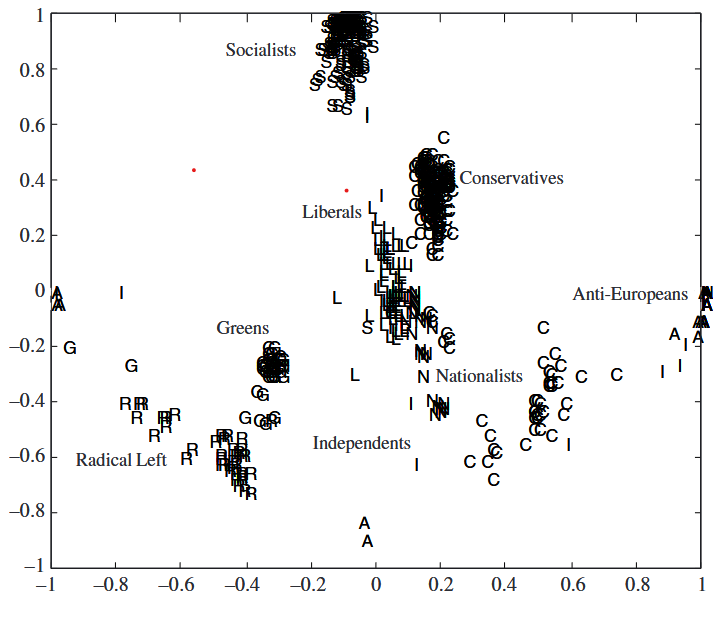
\includegraphics[width=0.65\textwidth]{Graphs/Screenshot 2024-06-09 220607}
        \caption{Ideal points estimates from Hix \& Noury (2009)}
        \label{fig:WNOMINATEHIX6}
    \end{figure}


    As we do not have access to the code used for the analysis done by Hix and Noury, we have to make
    assumptions as
    to the parameters that they chose. \( \beta \)
    and 'lop' have default values, heuristically assigned by the
    creators of the software, and researchers usually do not change those. The issue arises with the
    `polarity'
    parameter. It requires the researcher using the package to choose a 'conservative' MP and the
    algorithm will
    center the result around his final position - so if the `polarity' is chosen as (10,10), as it
    is in our case, \texttt{wnominate}
    will center the result around the 10th MEP in the dataset in dimension 1 and 10th MEP in dimension 2.
    There is
    no feasible way to recreate the result exactly without the knowledge of the MEP used as the
    `conservative'.
    However, this parameter does not distort the distribution of the ideal points, just their alignment and
    rotation
    - so the final product should be still comparable to the results achieved by Hix \& Noury.
    \ref{fig:WNOMINATEHIX6}

    \begin{figure}[H]
        \centering
        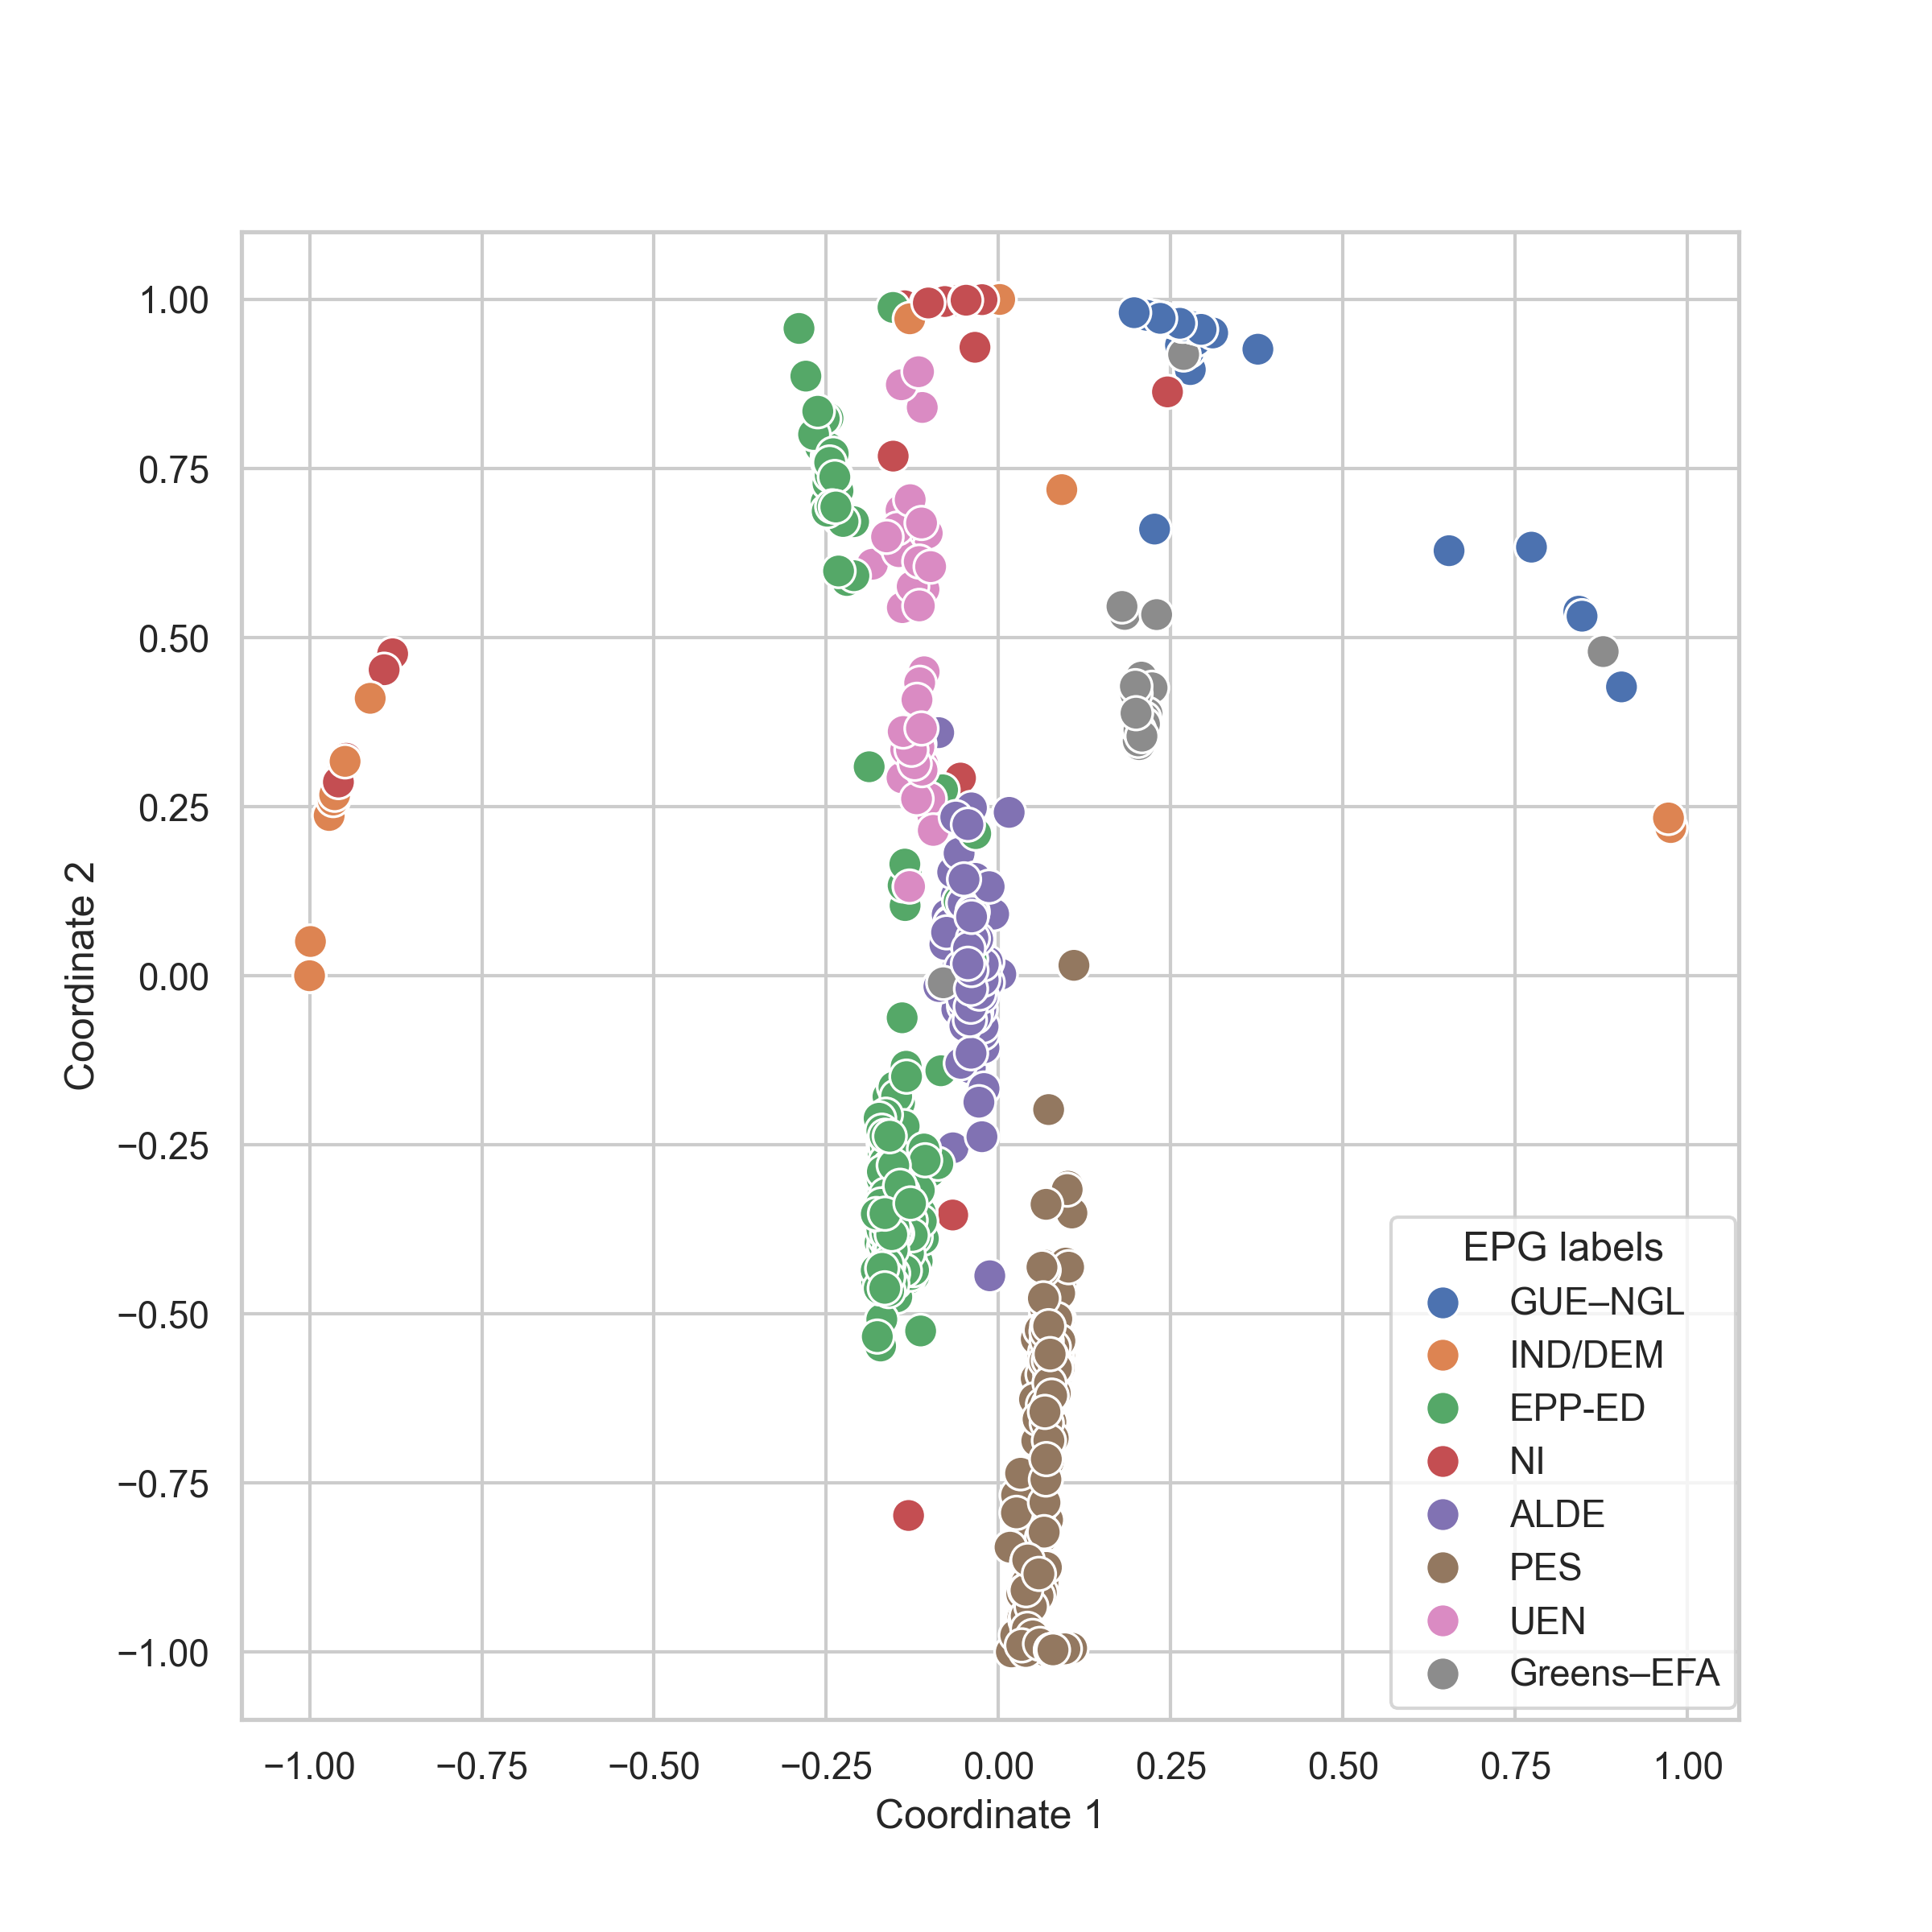
\includegraphics[width=0.65\textwidth]{Graphs/WNOMINATE2d}
        \caption{Recreation of Ideal Points Analysis in European Parliament 6 using WNOMINATE}
        \label{fig:WNOMINATE 6}
    \end{figure}



    \susbection{Comparison of results}
    In order to explicitly compare the results we achieved to the ones of Hix \& Noury (2009) we would need
    to have
    access to the original coordinates produced by W-NOMINATE in their research. This data is
    unfortunately not available publicly, so the most feasible method of comparison is visual analysis
    of characteristics of both representations of ideal points. One can immediately notice that the
    positions of the main political groups in our map are inverted in relation to the map we are
    comparing with. This is likely due to a different MEP being chosen as the `conservative' in the
    initialization of the algorithm. In order to compare the results more adequately, we decided to show
    a map with both dimensions inverted, to better match the original results.

    \begin{figure}[H]
        \centering
        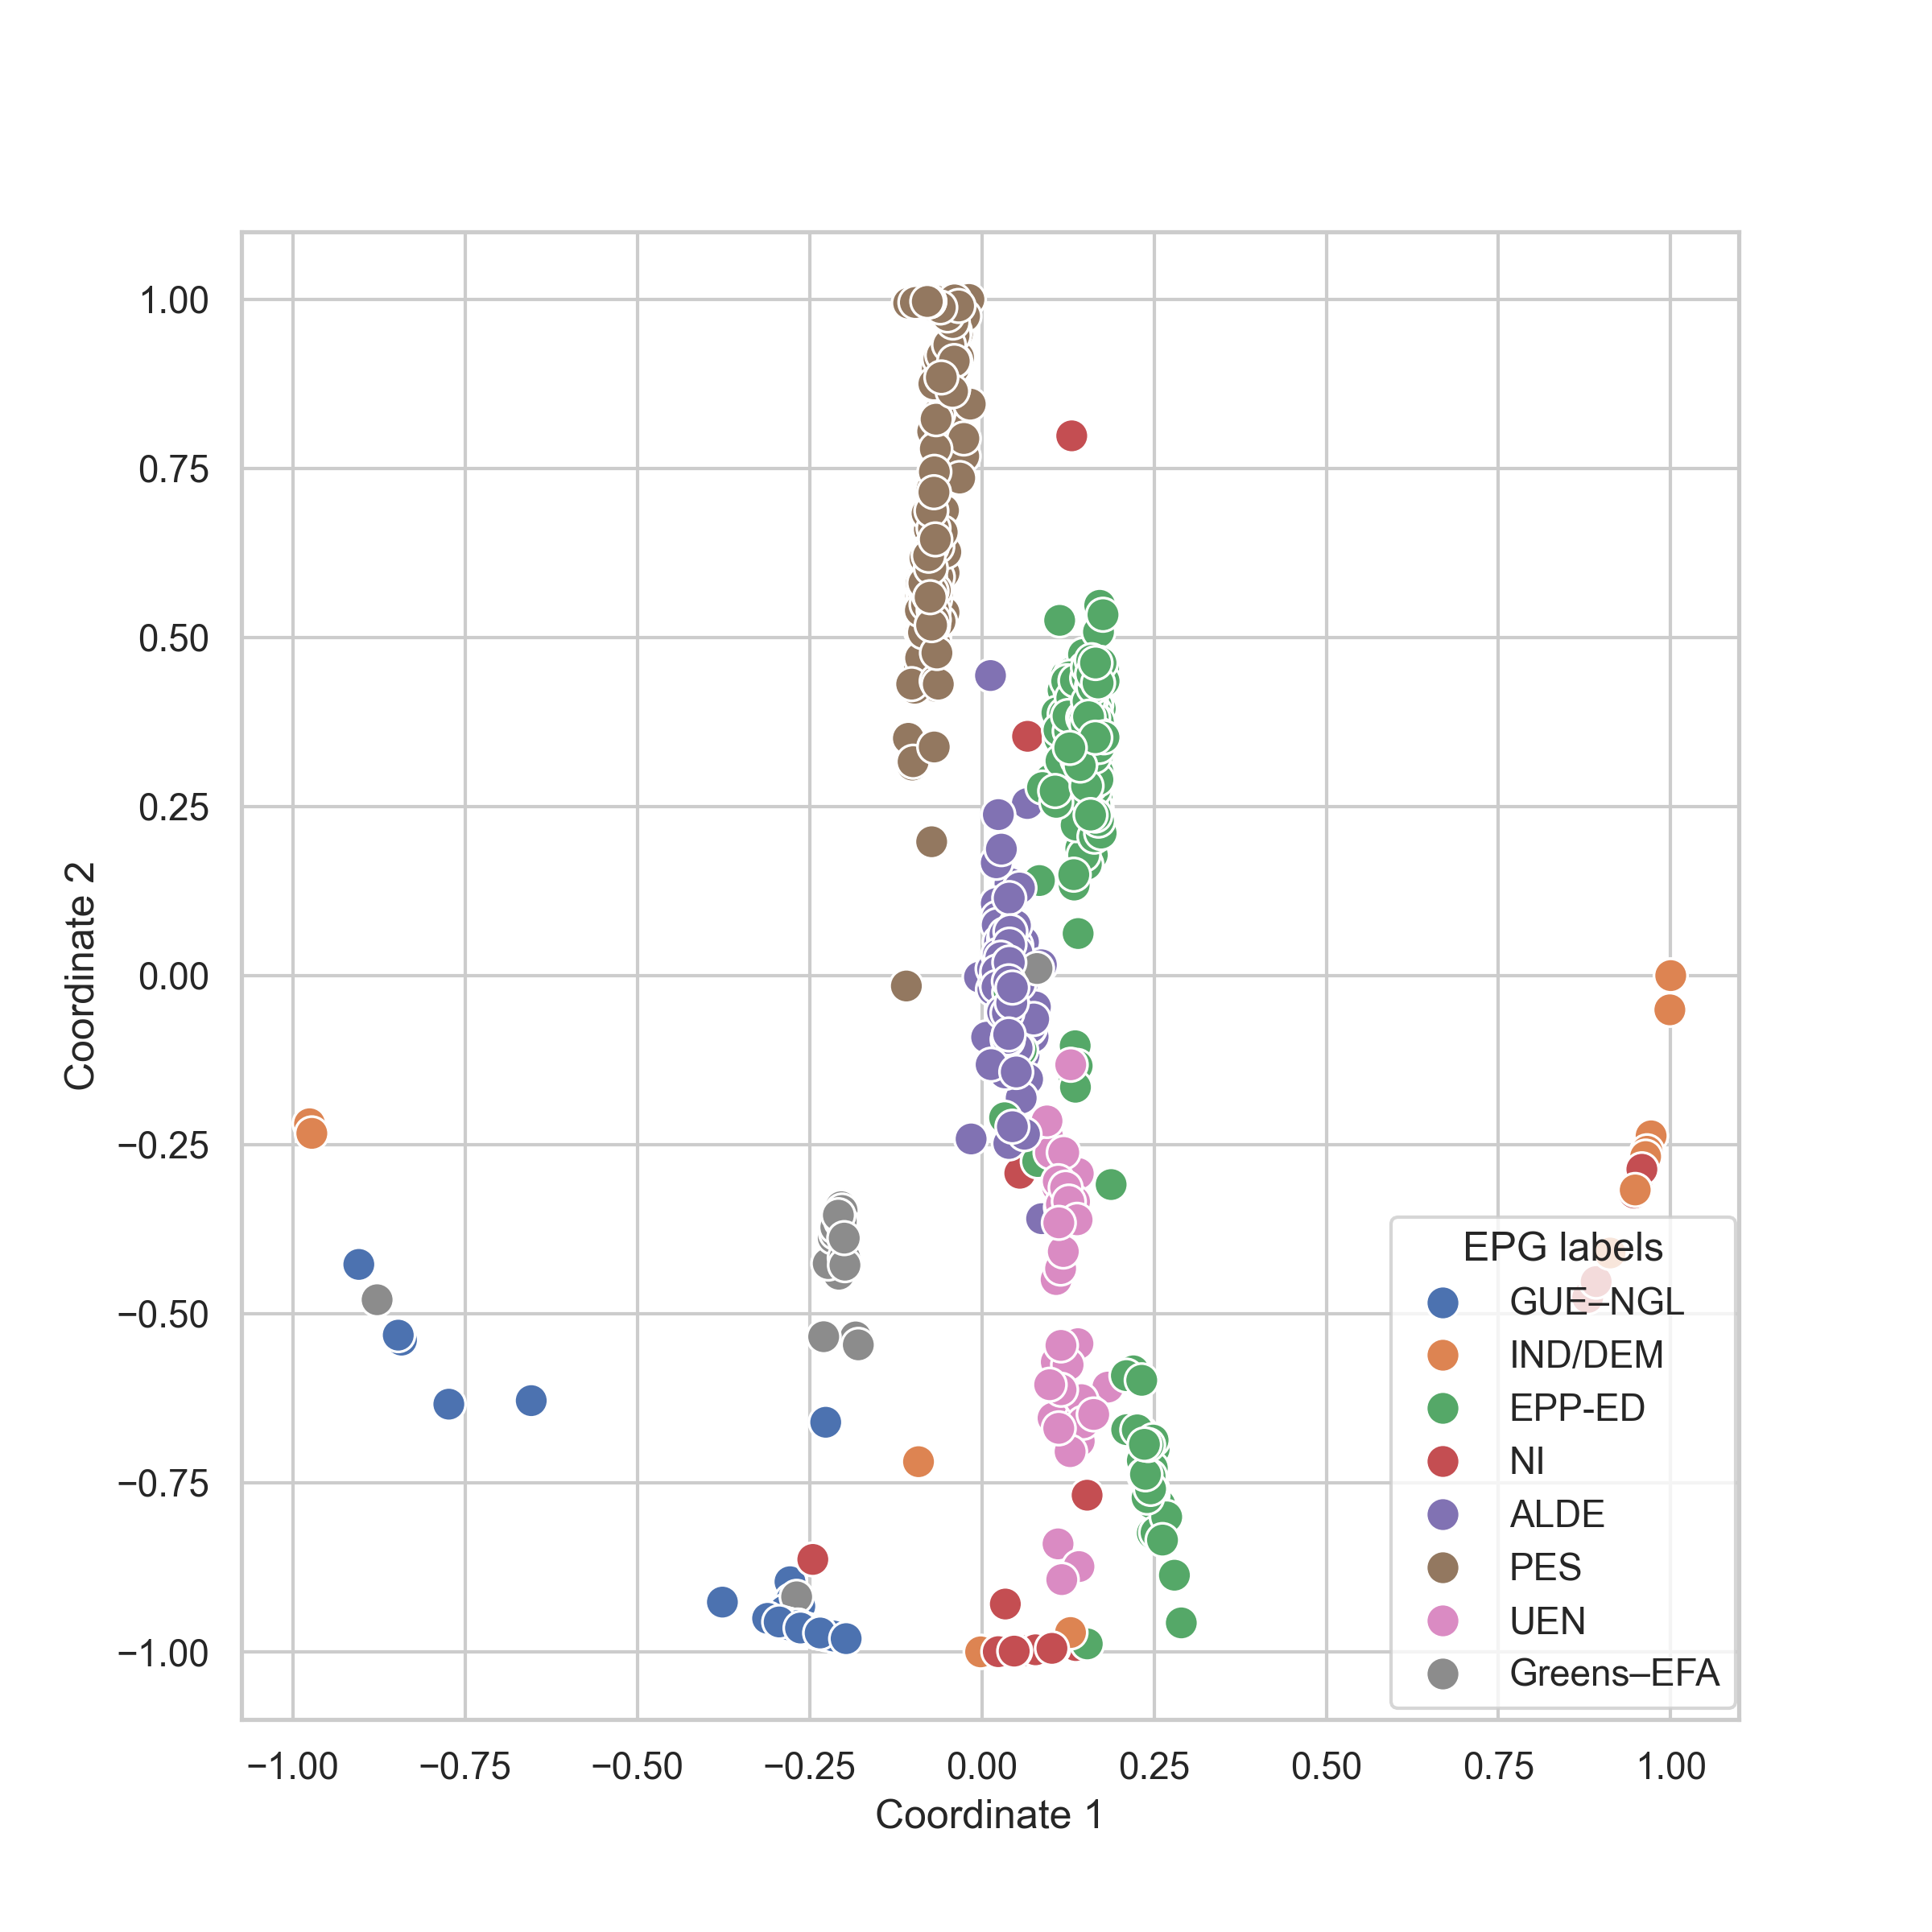
\includegraphics[width=0.65\textwidth]{Graphs/WNOMINATEflipped2d}
        \caption
        {Recreation of Ideal Points Analysis in European Parliament 6 using WNOMINATE with both dimensions
        inverted}
        \label{fig:WNOMINATE 6 FLIPPED}
    \end{figure}
    With maps aligned, several similar characteristics become apparent. The EPGs appear in similar
    clusters, with a similar alignment as in the original. The Socialists (PES in reproduction) are
    firmly in the range of
    -0.2 to 0 in the first dimension in both cases and 1 and 0.25 in the second dimension in the
    reproduction, but between 1 and 0.6 in the original work. The most likely explanation for this
    discrepancy is the polarity setting in the second dimension - if we chose a MEP that is closer to
    some of the
    Socialists in terms of ideal points than the one in Hix \& Noury (2009) as a `conservative' we would
    naturally
    bring the Socialists closer to the middle of the map, distorting the image. That seems to be the
    most competent explanation of this phenomenon. Again, however, we do not have a way of comparing the
    results directly and lack the knowledge of the `conservative' used in the reproduced work.

    Similarly to the Socialists, other groups - such as Conservatives (EPP-ED), Liberals (ALDE),
    Nationalists (UEN) and Greens (Greens-EFA) are in comparable clusters to the previous research. The
    Radical Left (GUE-NGL), the Anti-Europeans (IND/DEM) and the Independents (NI) are located on
    opposite spectra of the map, along the borders of the unit sphere (an inherent feature of maps
    produced by W-NOMINATE are points with maximum distance of 1 from the center). This also reflects
    accurately the reproduced work.

    With such similar results, and without other means of confirming the similarity, we can plausibly
    establish a successful reproduction of the workflow that was used in Hix & Nouury (2009). This
    results allows us to conclude the integrity of the dataset and methods used.


    \section{Comparison of one-dimensional ideal points methods}
    \label{sec:comparison-of-one-dimensional-ideal-points-methods}
    As mentioned before, W-NOMINATE has some limitations - when computing ideal points with a greater number
    of datapoints, it becomes 'prohibitively slow' (Imai,Lo 2016), so much so, that we were not able to
    calculate ideal points (neither in one-dimensional, nor two-dimensional space) for a larger dataset of
    European Parliament 9. In order to circumvent those limitations,
    in 2016 Kosuke, Imai and Lo developed a software which achieves similar results to W-NOMINATE, while
    remaining computationally efficient, as discussed in Chapter 4.

    THe main drawback of emIRT is lack of support for more than one dimension. Despite this, we set out to
    test the results from this alternative method, as the computational improvements may prove useful for analysis
    in the context of the European Parliament.
    \begin{figure}[H]
        \centering
        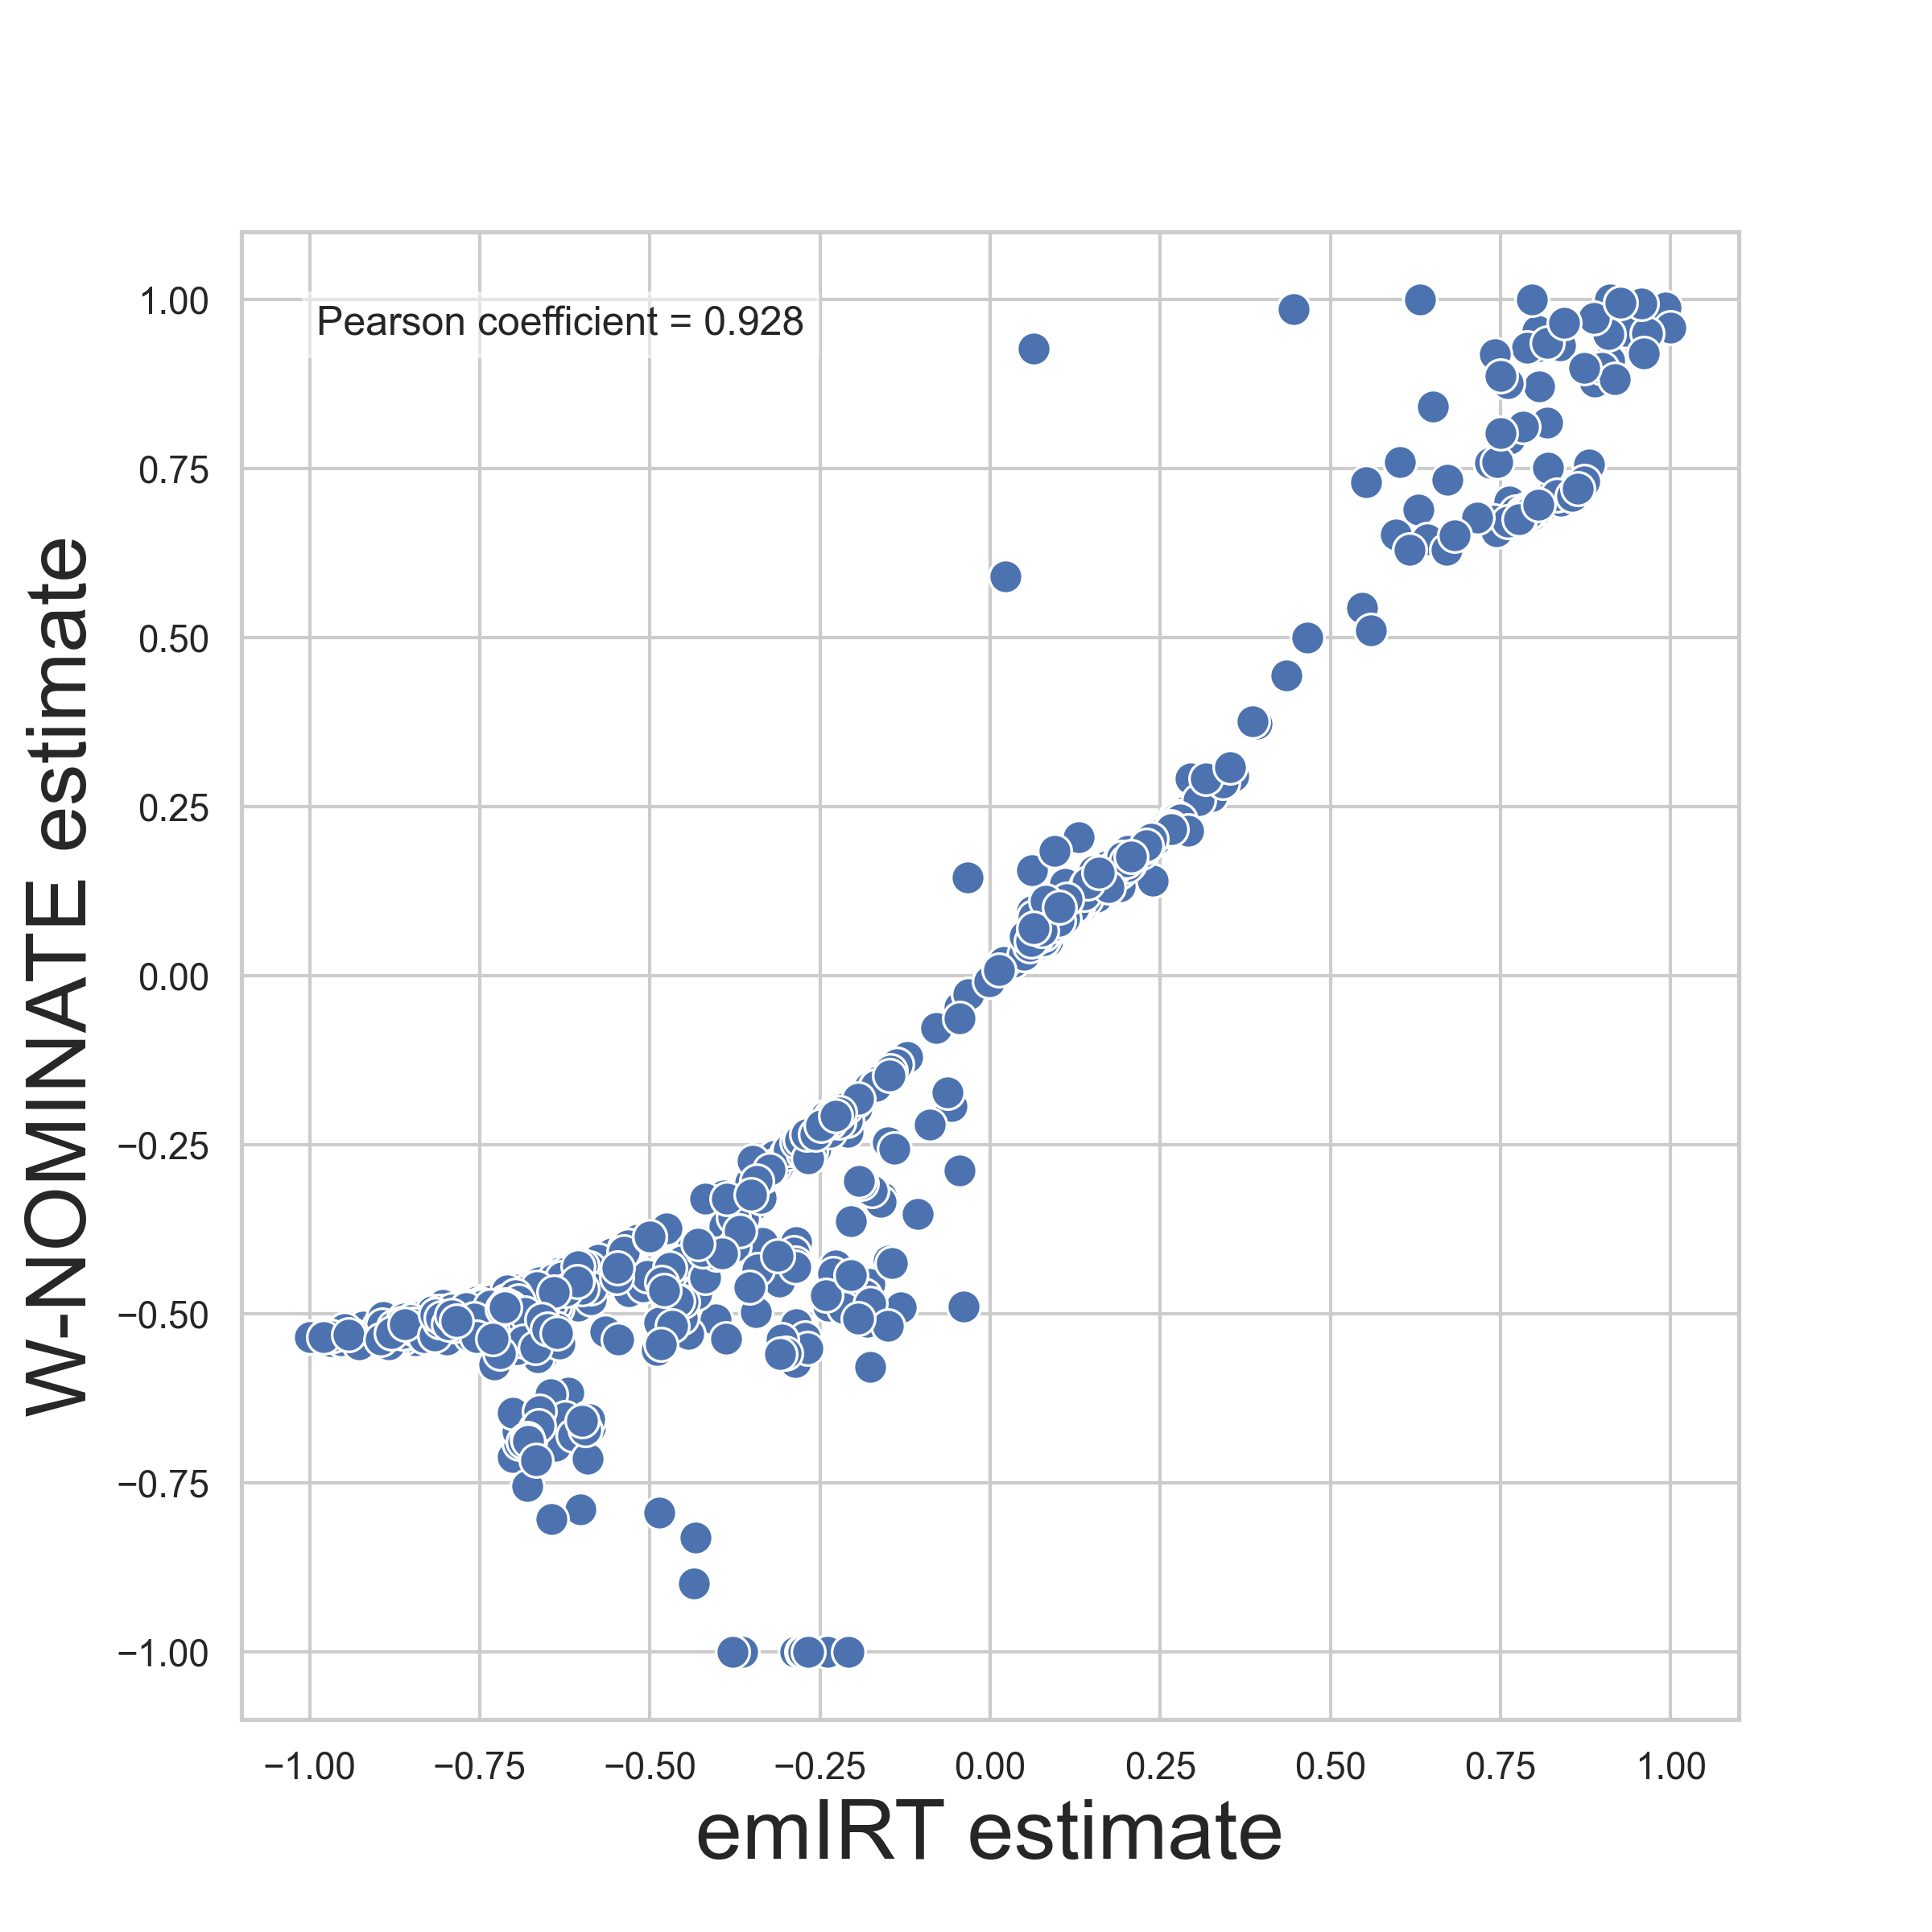
\includegraphics[width=0.65\textwidth]{Graphs/ScatterWNOMINATE_6}
        \caption{Scatter plot of W-NOMINATE and emIRT estimations of ideal points in EP6}
        \label{fig:WNOMINATE_SCATTER_6}
    \end{figure}

    \begin{figure}[H]
        \centering
        \begin{subfigure}[b]{0.48\textwidth}
            \centering
            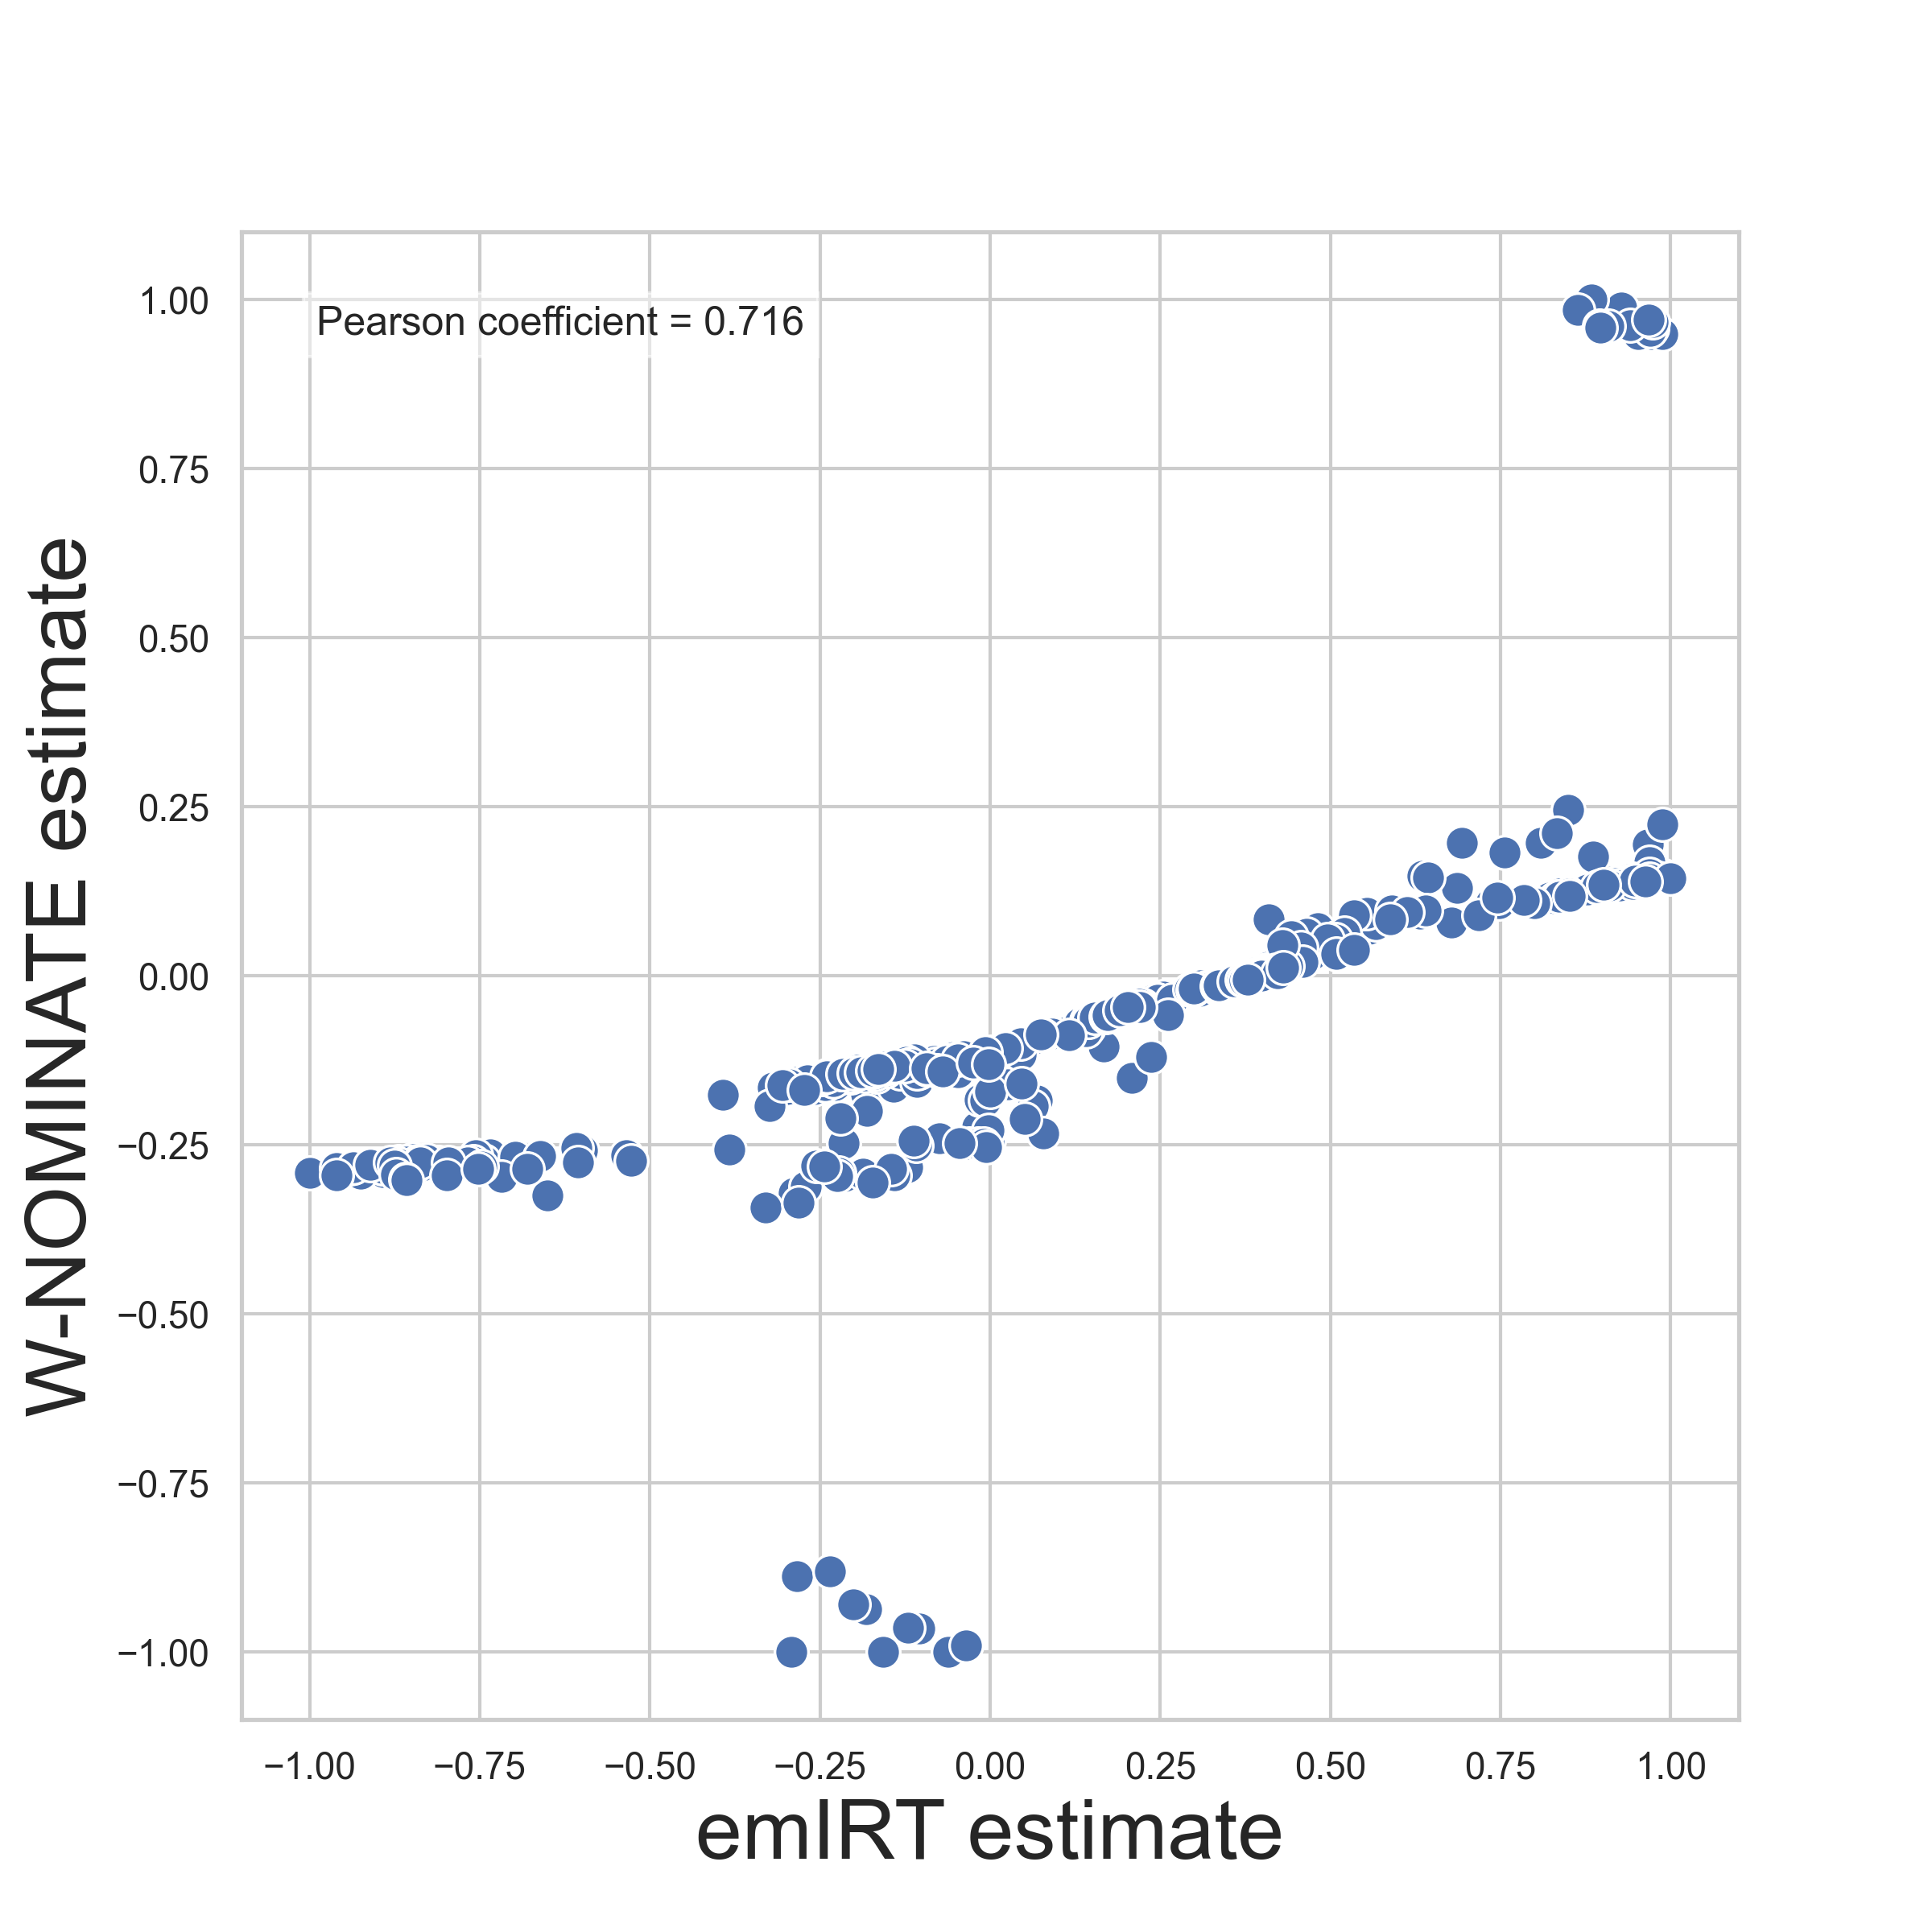
\includegraphics[width=\textwidth]{Graphs/ScatterWNOMINATE_7}
            \caption{W-NOMINATE and emIRT in EP7}
            \label{fig:WNOMINATE_SCATTER_7}
        \end{subfigure}
        \hfill
        \begin{subfigure}[b]{0.48\textwidth}
            \centering
            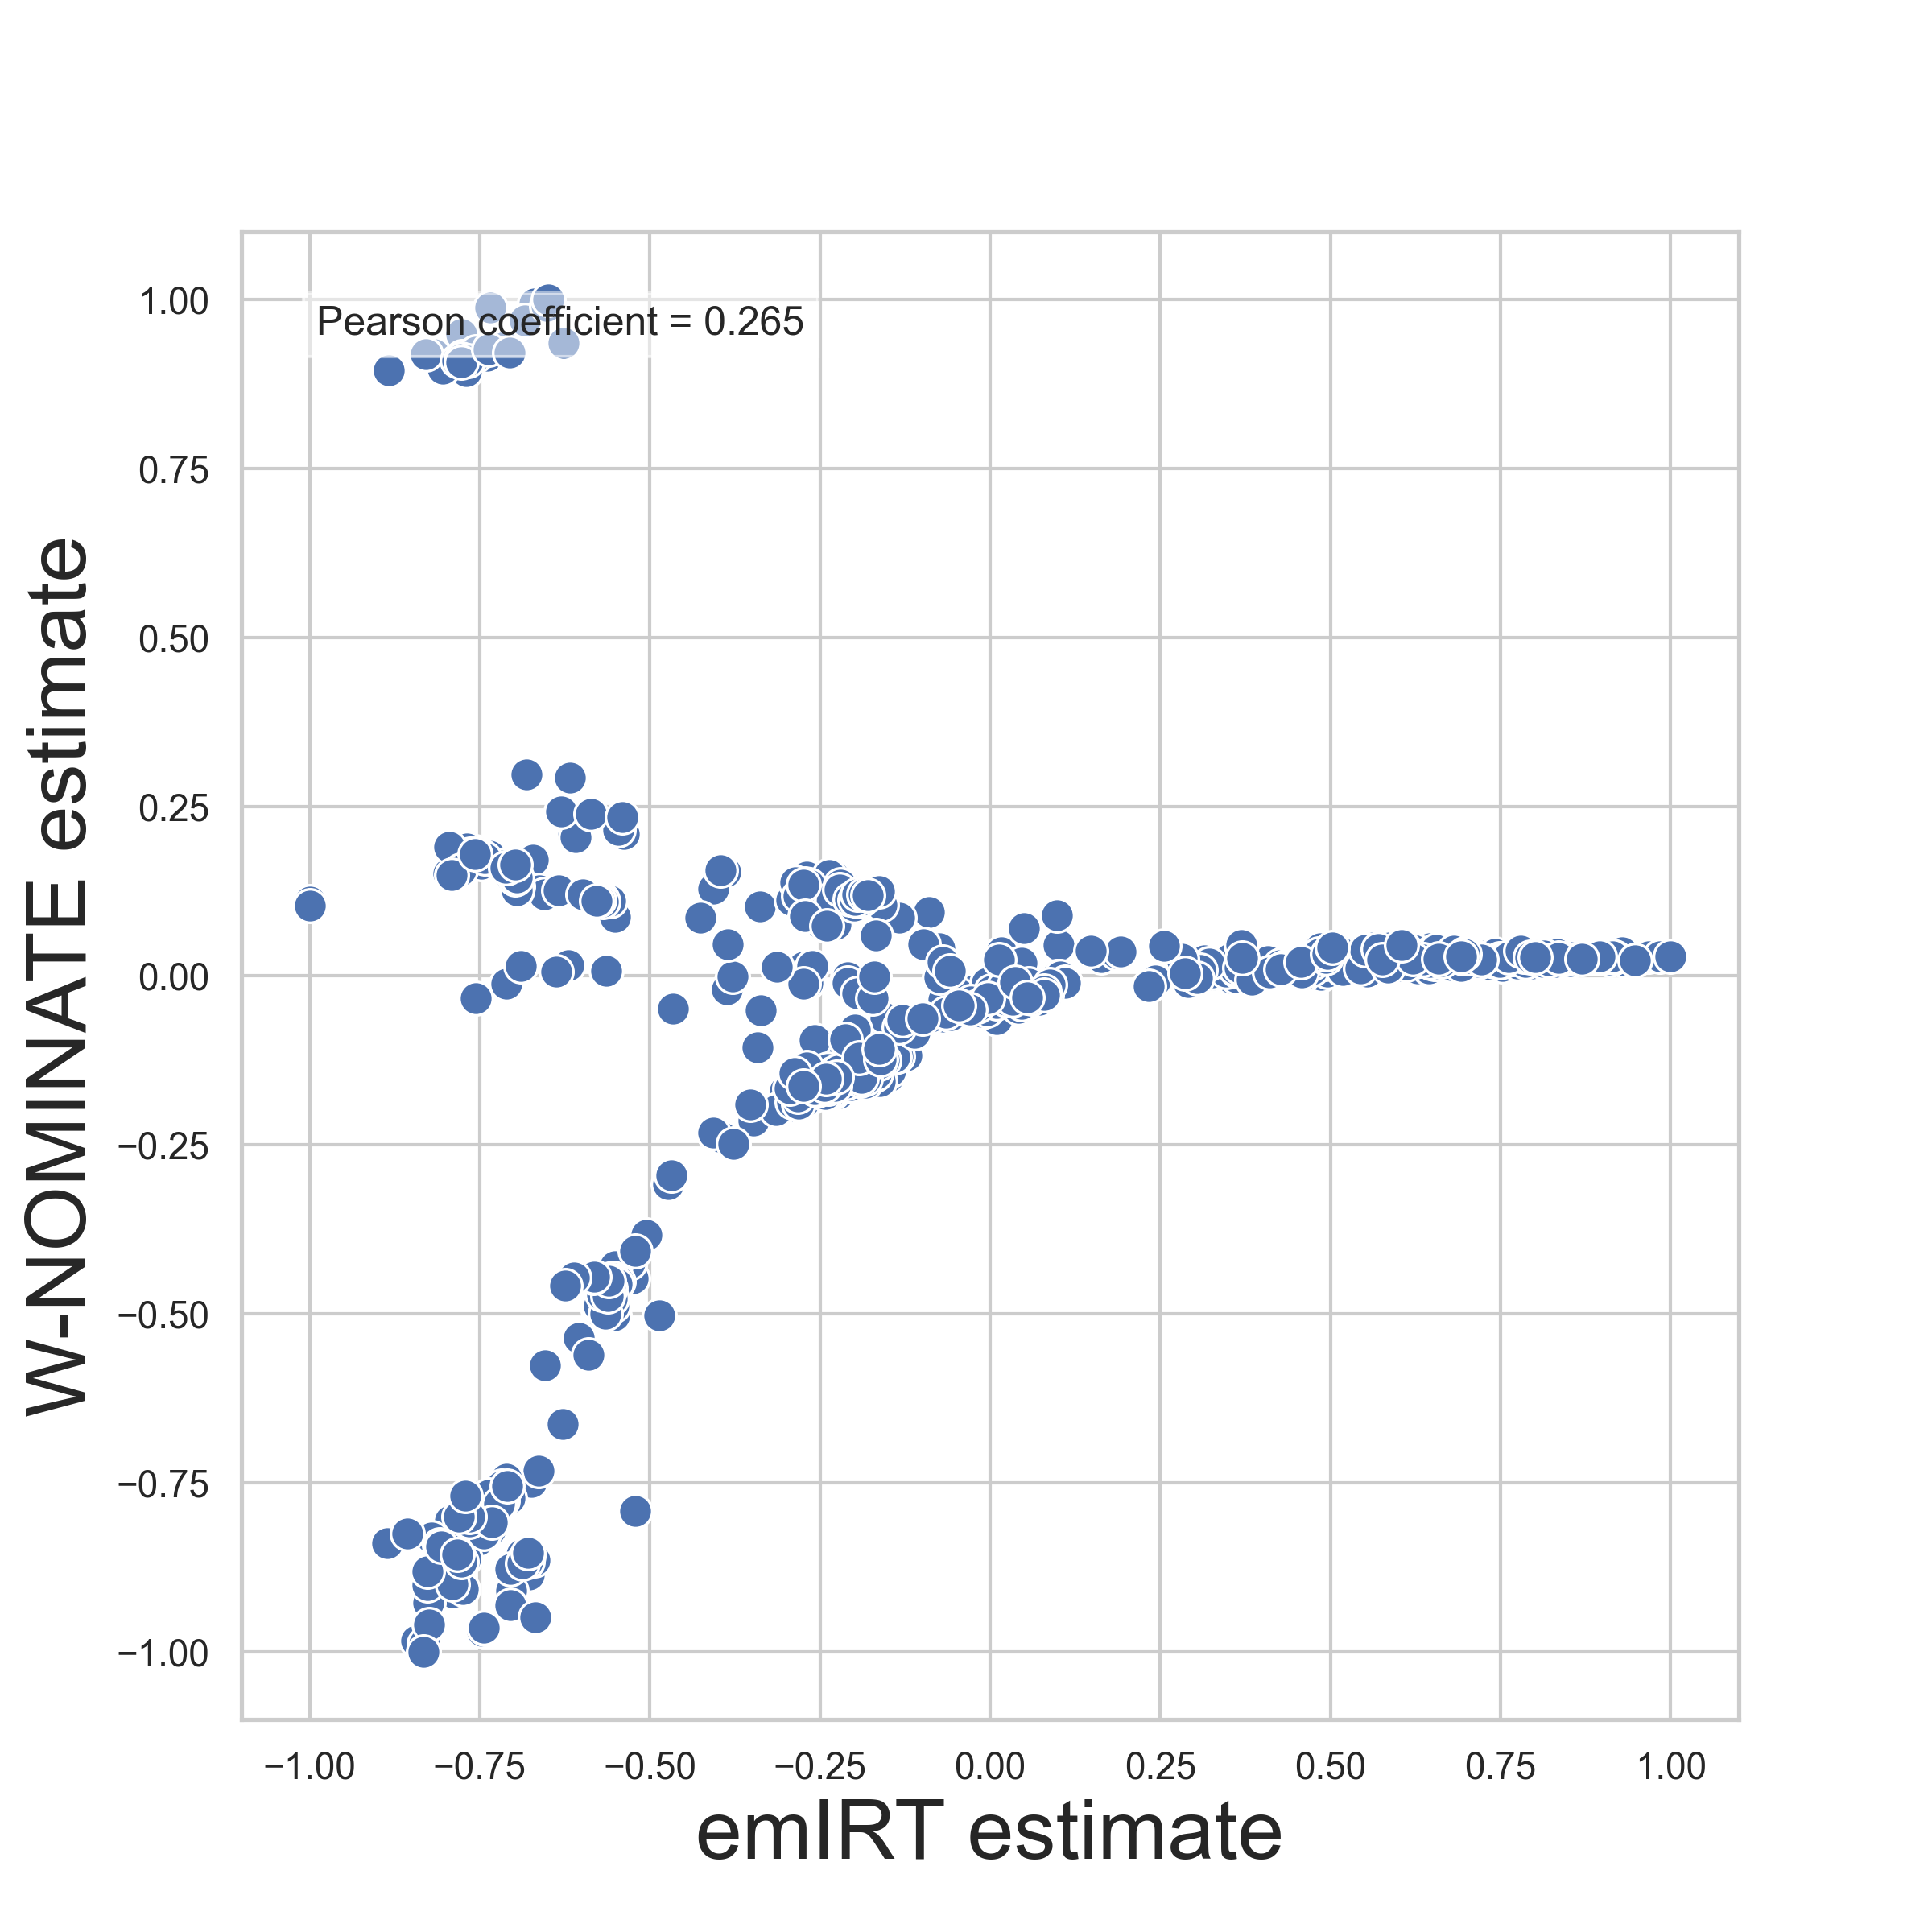
\includegraphics[width=\textwidth]{Graphs/ScatterWNOMINATE_8}
            \caption{W-NOMINATE and emIRT in EP8}
            \label{fig:WNOMINATE_SCATTER_8}
        \end{subfigure}
        \caption{Scatter plots of W-NOMINATE and emIRT estimations of ideal points in EP7 and EP8}
        \label{fig:WNOMINATE_SCATTER_7_8}
    \end{figure}

    \subsection{emIRT}
    The procedure for initializing emIRT is similar to W-NOMINATE - with one crucial difference, starting points.
    Unlike W-NOMINATE, which calculates estimated starting positions using the eigenvectors of the agreement matrix,
    emIRT randomly generates them. The \texttt{emIRT} package for \texttt{R} includes a built in function to obtain
    the starts.
    The user has a choice between two options for generating the initialization parameters: `zeroes' and
    `random'.
    In both options the starting points are drawn from a normal distribution.

    The difference between the two settings is the \(\alpha\) (difficulty) and \(\beta_j\)
    (discrimination) parameters.
    They determine,respectively, how difficult a specific roll-cal is for a specific MP to support, given their ideal
    point, and how
    much the preferences of an MP (ideal point) impacts (discriminates) their decision on how to vote on a specific
    issue.
    In `zeroes', both of these parameters start as zeroes, and in `random' they are drawn from a normal
    distribution.

    The default parameter is `zeroes', so, as suggested by the creators, we used the default in our initialization.
    To ensure compatibility with W-NOMINATE results, we anchored the results around the same MEP as in the
    W-NOMINATE case (the `anchor' parameter being an emIRT replacement of W-NOMINATE's `polarity').

    \subsection{W-NOMINATE}
    The procedure to estimate one-dimensional ideal points with W=NOMINATE is similar to the two-dimensional case.
    The practical difference is the parameter `dims' (dimensions), that by default is set to 2.
    In this case, we set it to 1, to produce one-dimensional results.
    The rest of the procedure is exactly as in the previous case.
    We were able to produce results for all parliaments, apart from EP9, where the dataset proved to big for W-NOMINATE
    to process.

    \begin{figure}[H]
        \centering
        \begin{subfigure}[b]{0.48\textwidth}
            \centering
            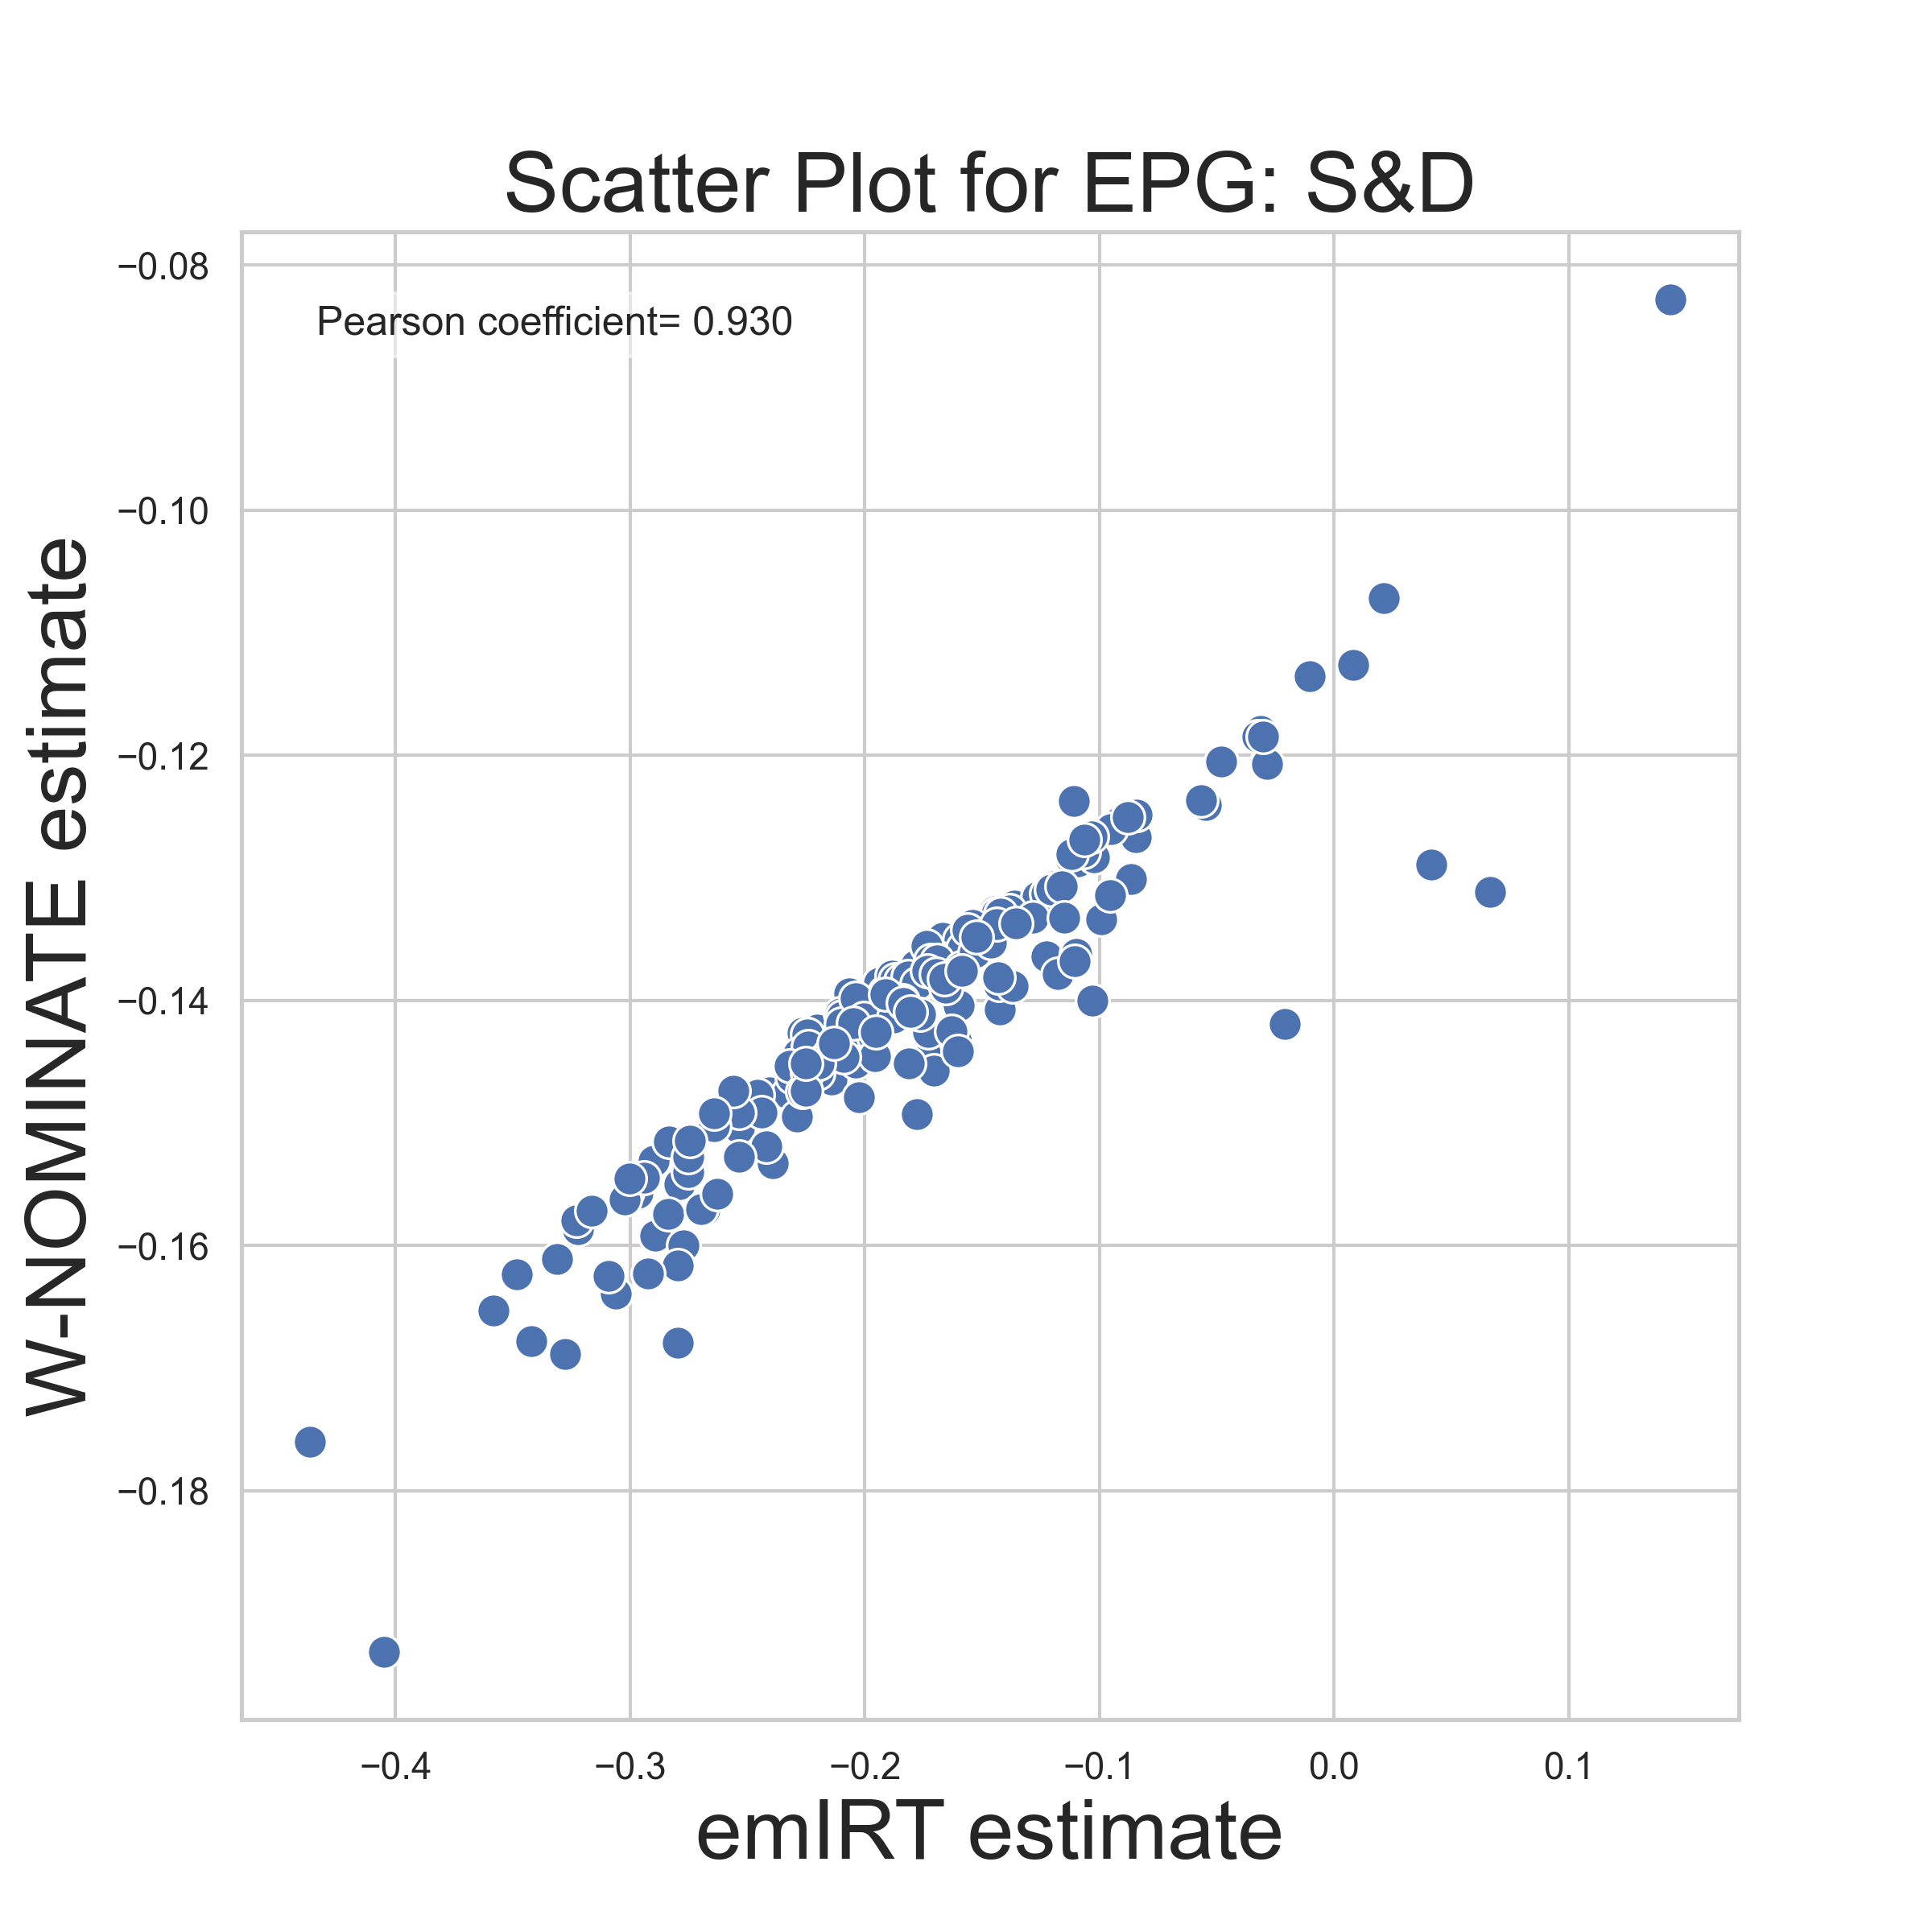
\includegraphics[width=\textwidth]{Graphs/ScatterEMWNOMINATE_7_EPG_S&D}
            \caption{W-NOMINATE and emIRT in EP7 (S\&D)}
            \label{fig:WNOMINATE_S&DSCATTER_7}
        \end{subfigure}
        \hfill
        \begin{subfigure}[b]{0.48\textwidth}
            \centering
            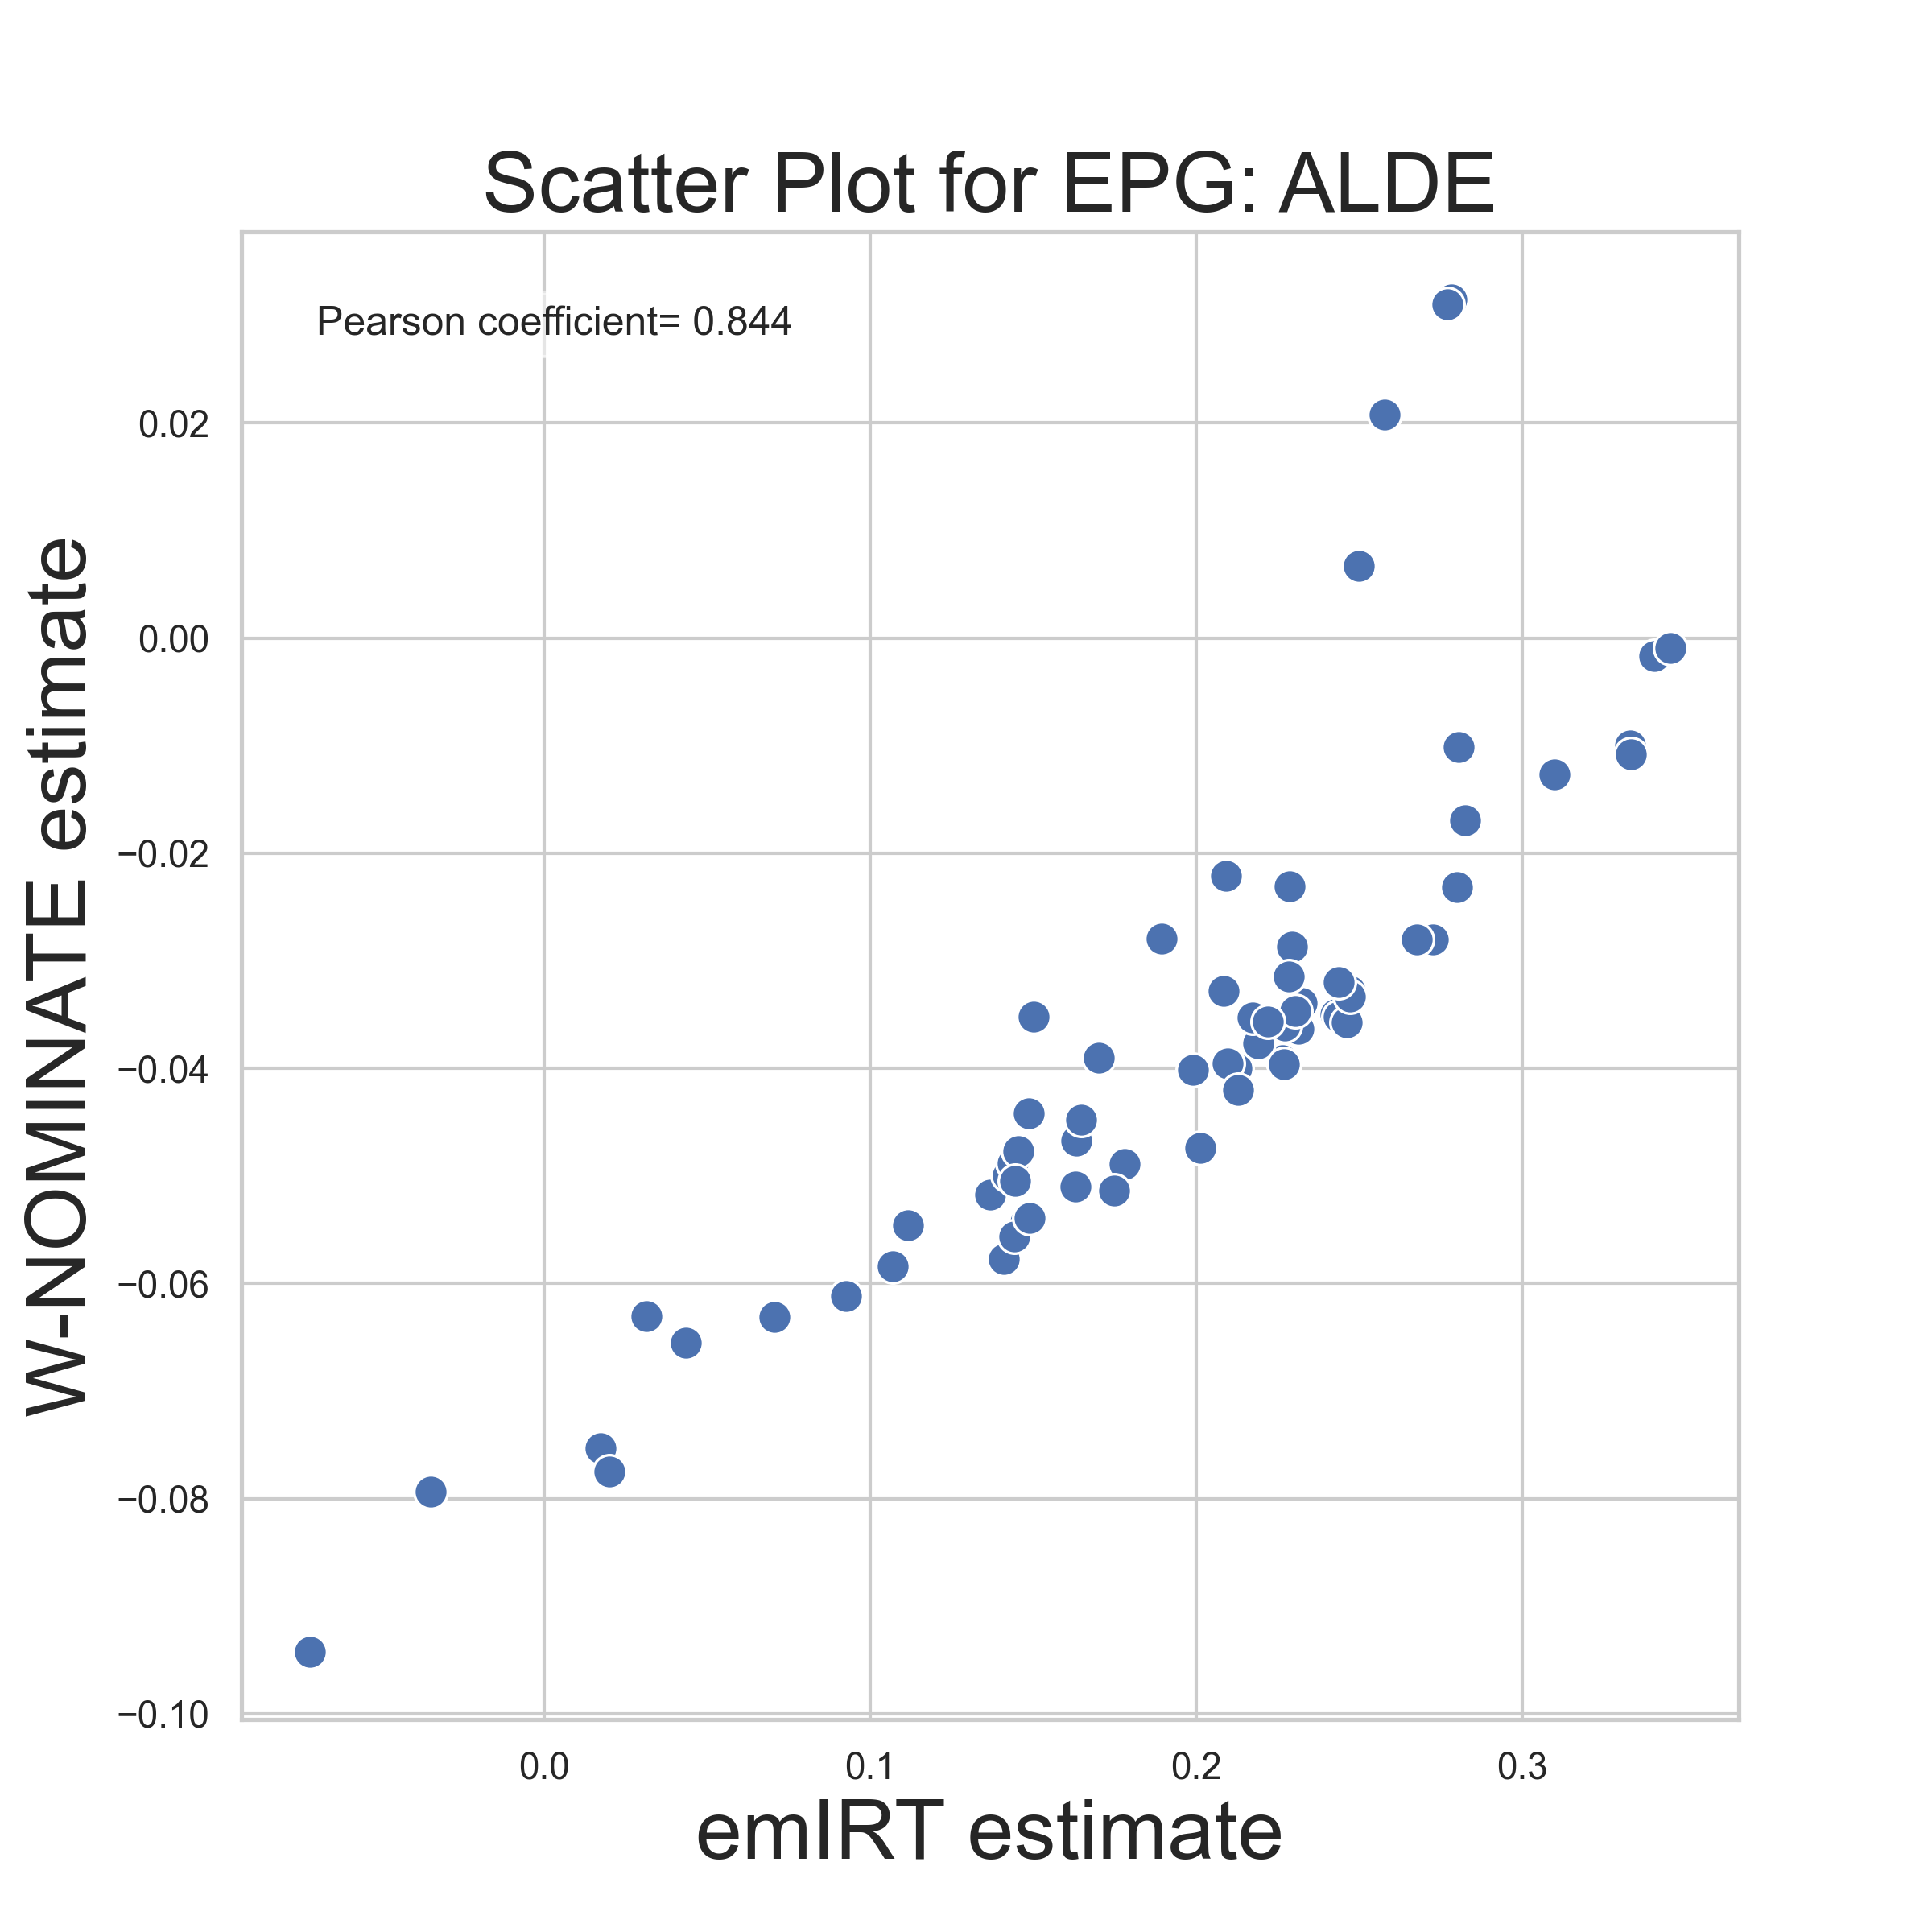
\includegraphics[width=\textwidth]{Graphs/ScatterEMWNOMINATE_8_EPG_ALDE}
            \caption{W-NOMINATE and emIRT in EP8 (ALDE)}
            \label{fig:WNOMINATE_ALDESCATTER_8}
        \end{subfigure}
        \caption{Scatter plots of W-NOMINATE and emIRT estimations of ideal points in EP7 and EP8 for ALDE and S&D}
        \label{fig:WNOMINATE_SCATTER_parties}
    \end{figure}

    \begin{figure}[H]
        \centering
        \begin{subfigure}[b]{0.48\textwidth}
            \centering
            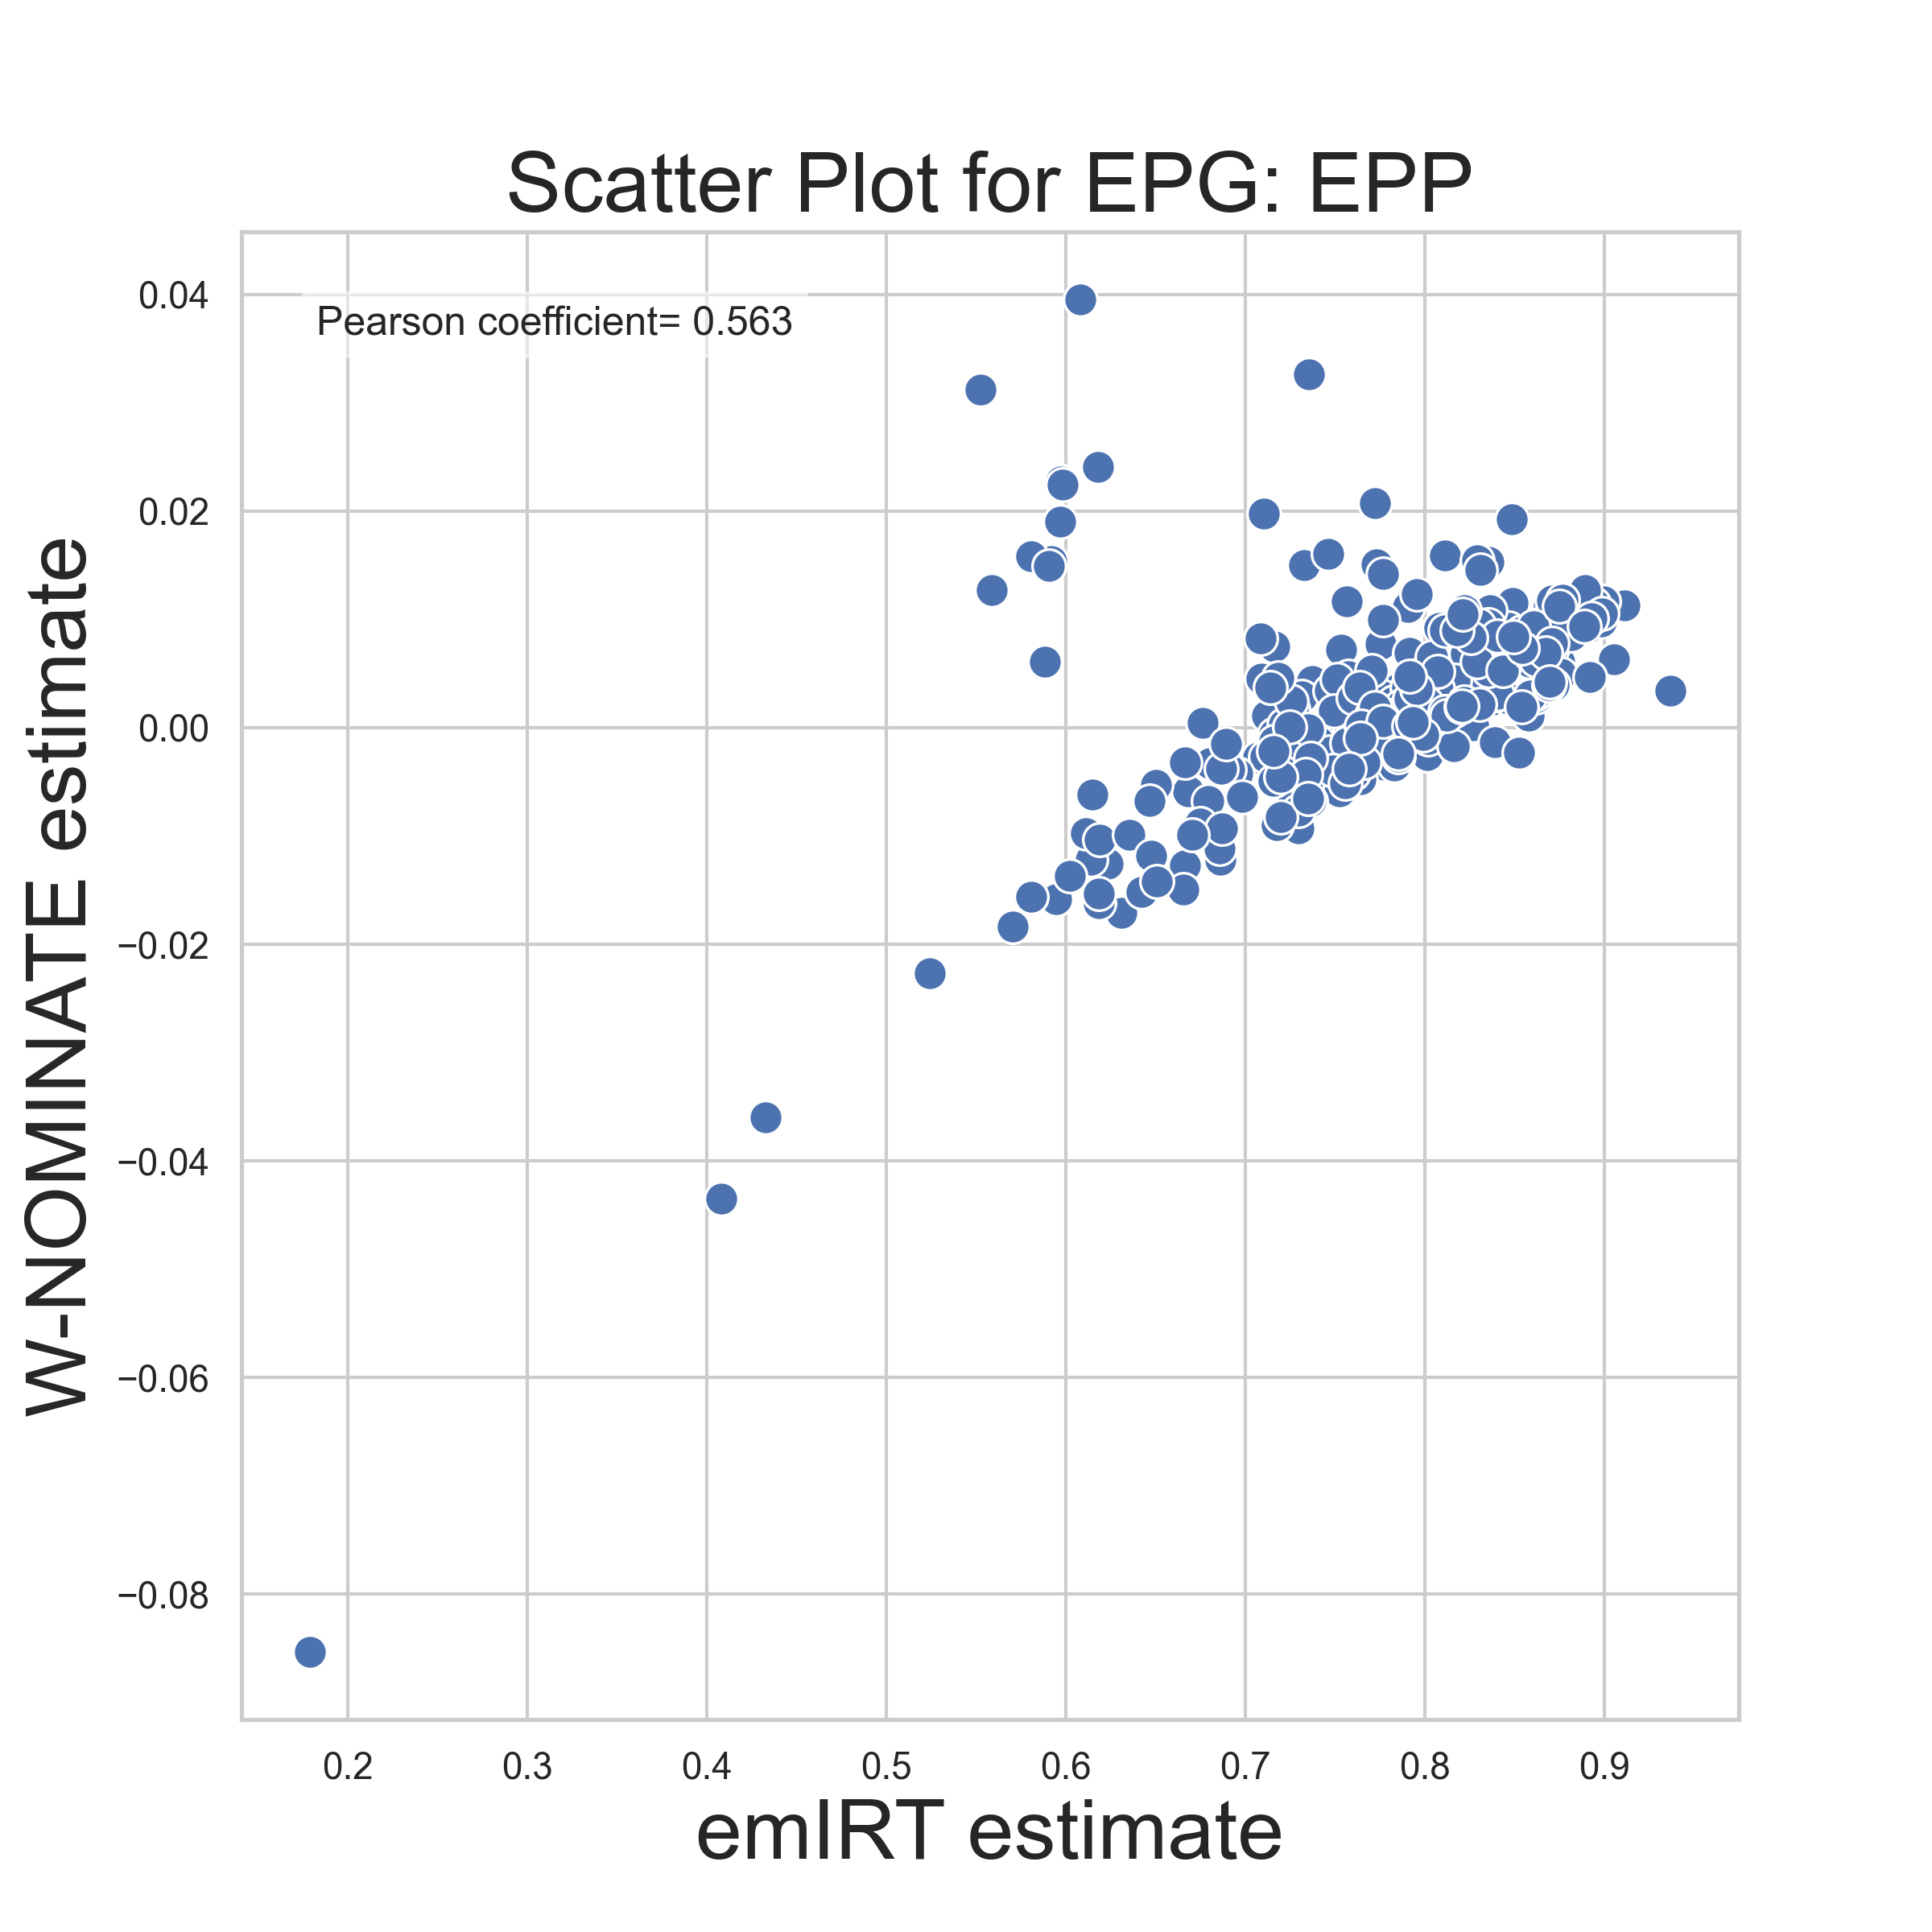
\includegraphics[width=\textwidth]{Graphs/ScatterEMWNOMINATE_7_EPG_EPP}
            \caption{W-NOMINATE and emIRT in EP7 (EPP)}
            \label{fig:WNOMINATE_EPP_SCATTER_7}
        \end{subfigure}
        \hfill
        \begin{subfigure}[b]{0.48\textwidth}
            \centering
            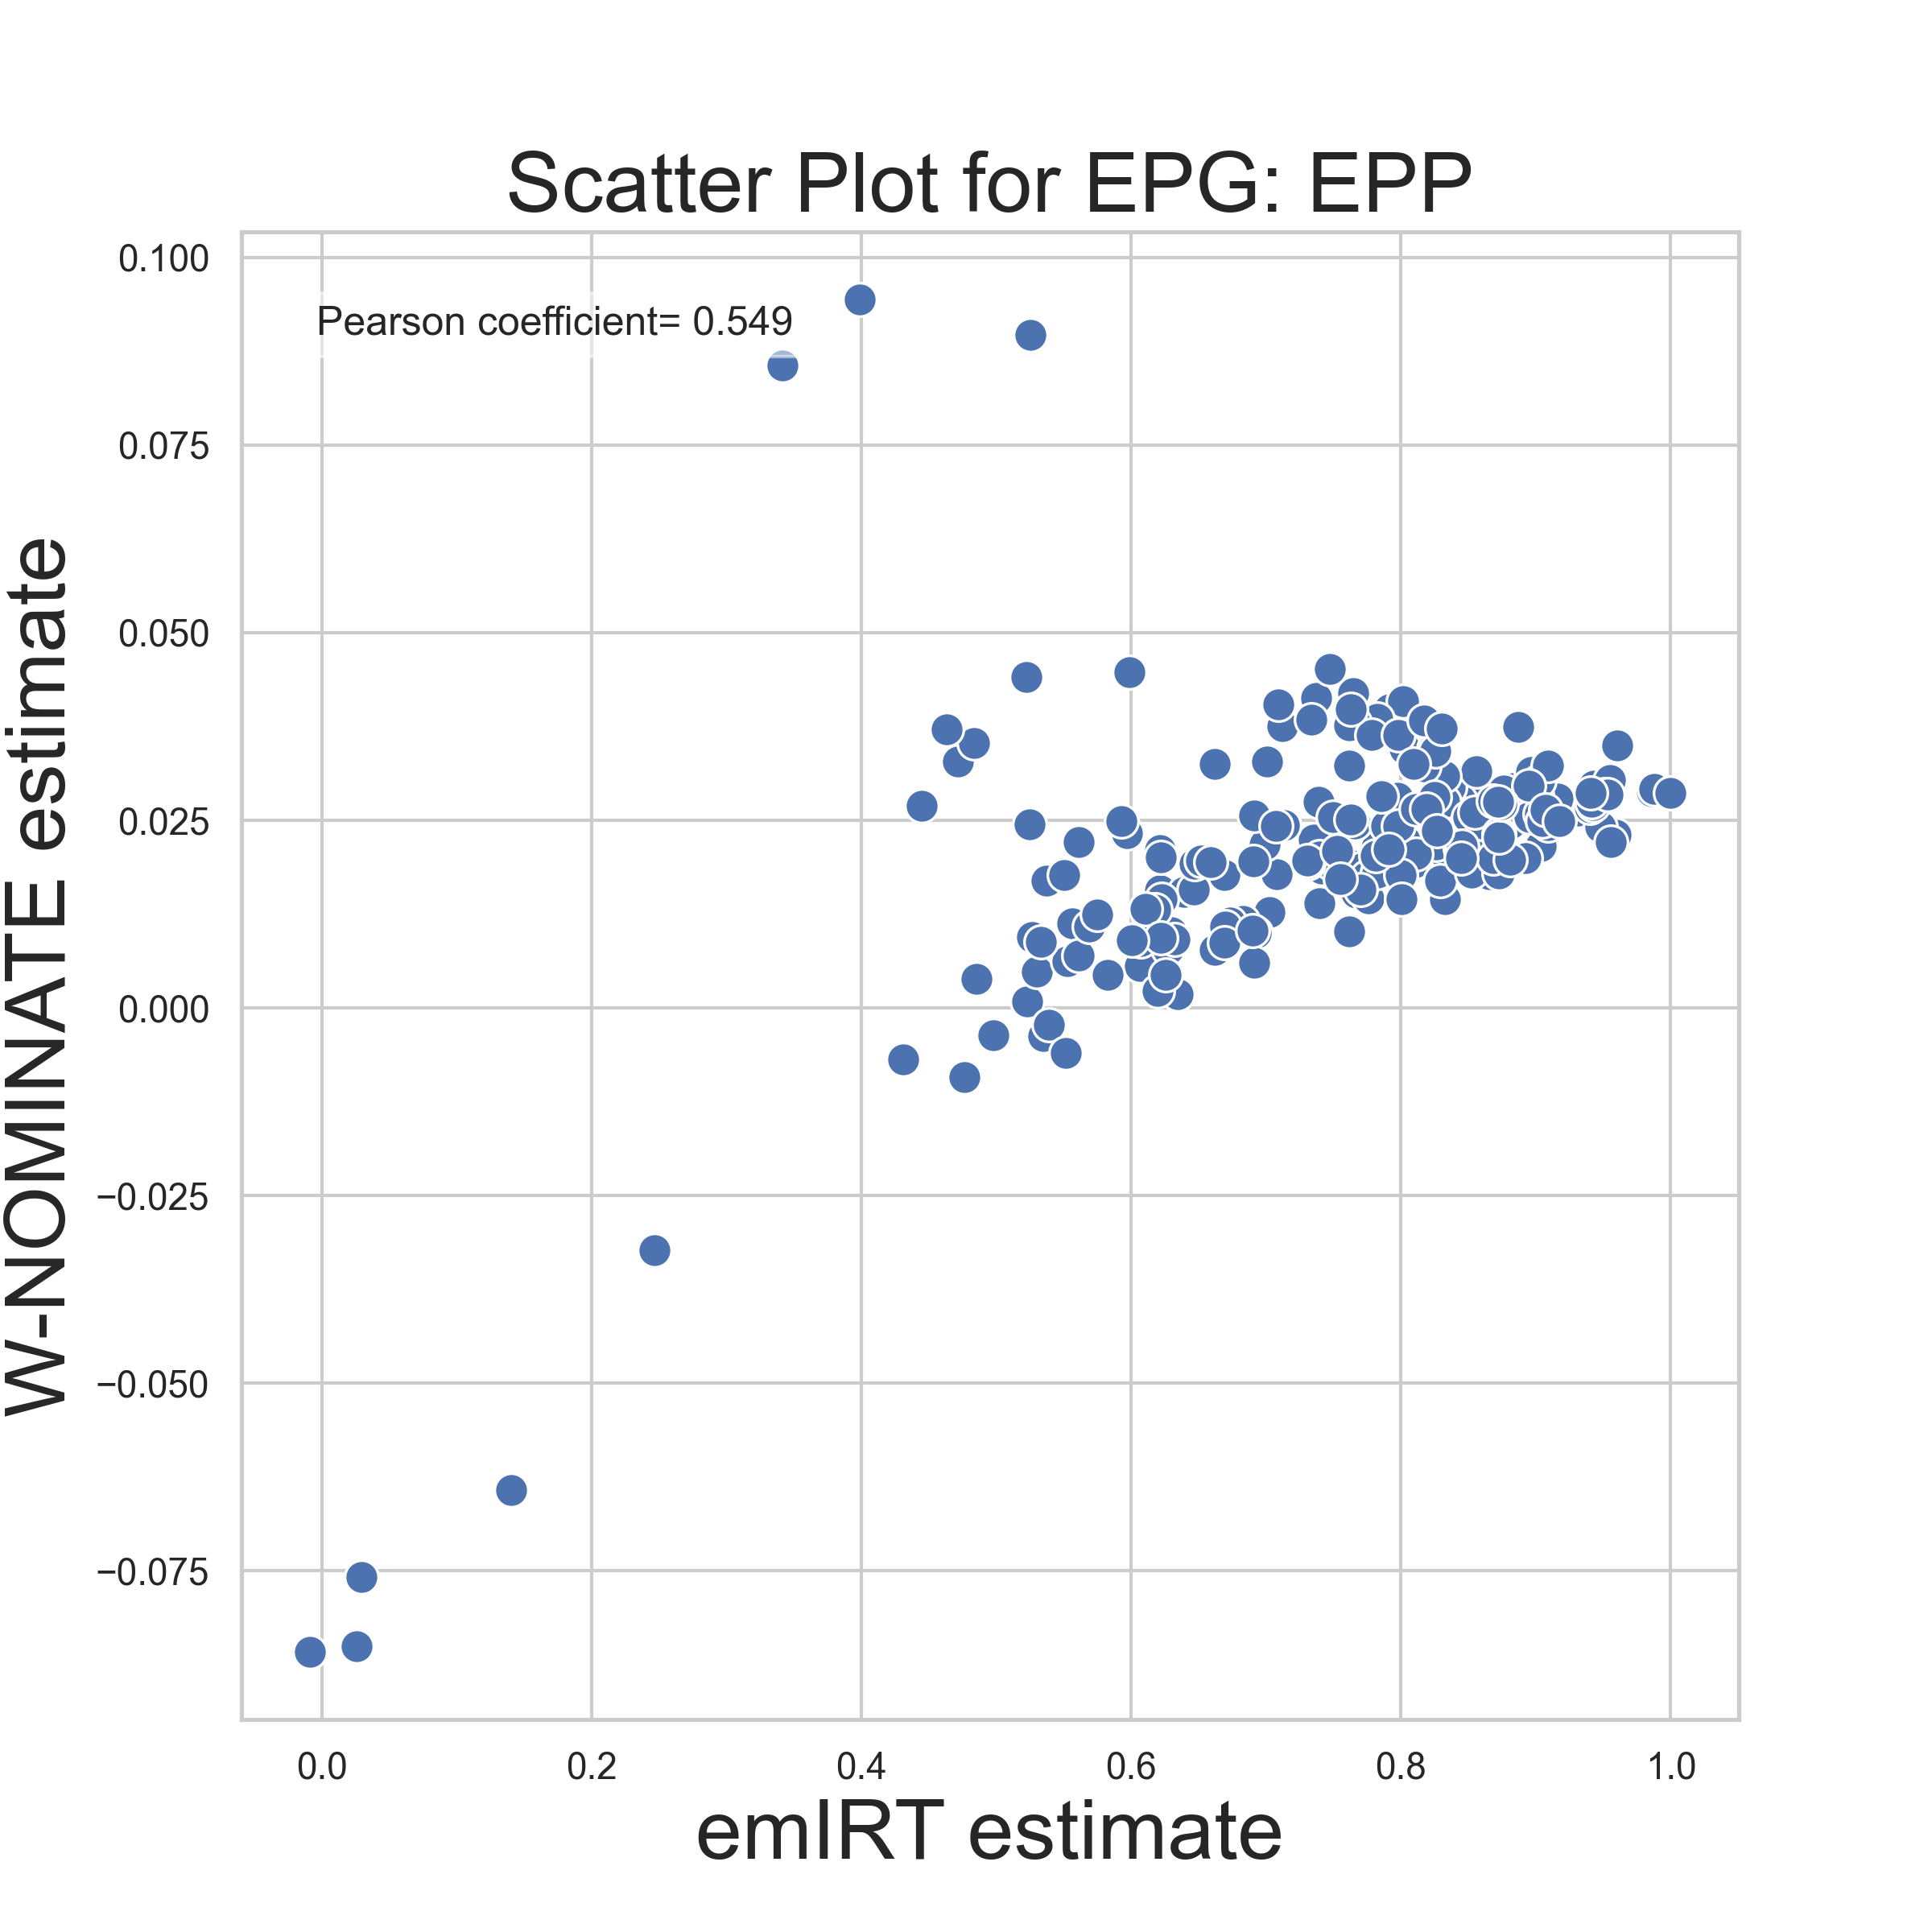
\includegraphics[width=\textwidth]{Graphs/ScatterEMWNOMINATE_8_EPG_EPP}
            \caption{W-NOMINATE and emIRT in EP8 (EPP)}
            \label{fig:WNOMINATE_EPPSCATTER_8}
        \end{subfigure}
        \caption{Scatter plots of W-NOMINATE and emIRT estimations of ideal points in EP7 and EP8 for EPP}
        \label{fig:WNOMINATE_SCATTER_EPP}
    \end{figure}

    \subsection{Comparison}
    In order to validate the results, we used the methodology that Kosuke, Imai and Lo (2016) used in their
    publication.
    The first step is to normalize the results to the same scale.
    By default, the ideal points produced by emIRT are in range of approximately [-10,10].
    We normalize the results to [-1,1] in order to match the scale of W-NOMINATE. After this step, we can create a
    scatterplot of the two results and calculate their Pearson
    coefficient.

    The results in EP 6 are as expected, with a Pearson correlation coefficient of 0.92, the results are comparable
    and can be used interchangeably, replicating the results Kosuke, Imai and Lo had in the case of the 112th US
    Congress.
    However, the results for EP7 and EP8 are surprising.
    With respective Pearson coefficients of 0.65 for EP7 and 0.61 for EP8, the results differ greatly from expectations.
    \begin{figure}[H]
        \centering
        \begin{subfigure}[b]{0.48\textwidth}
            \centering
            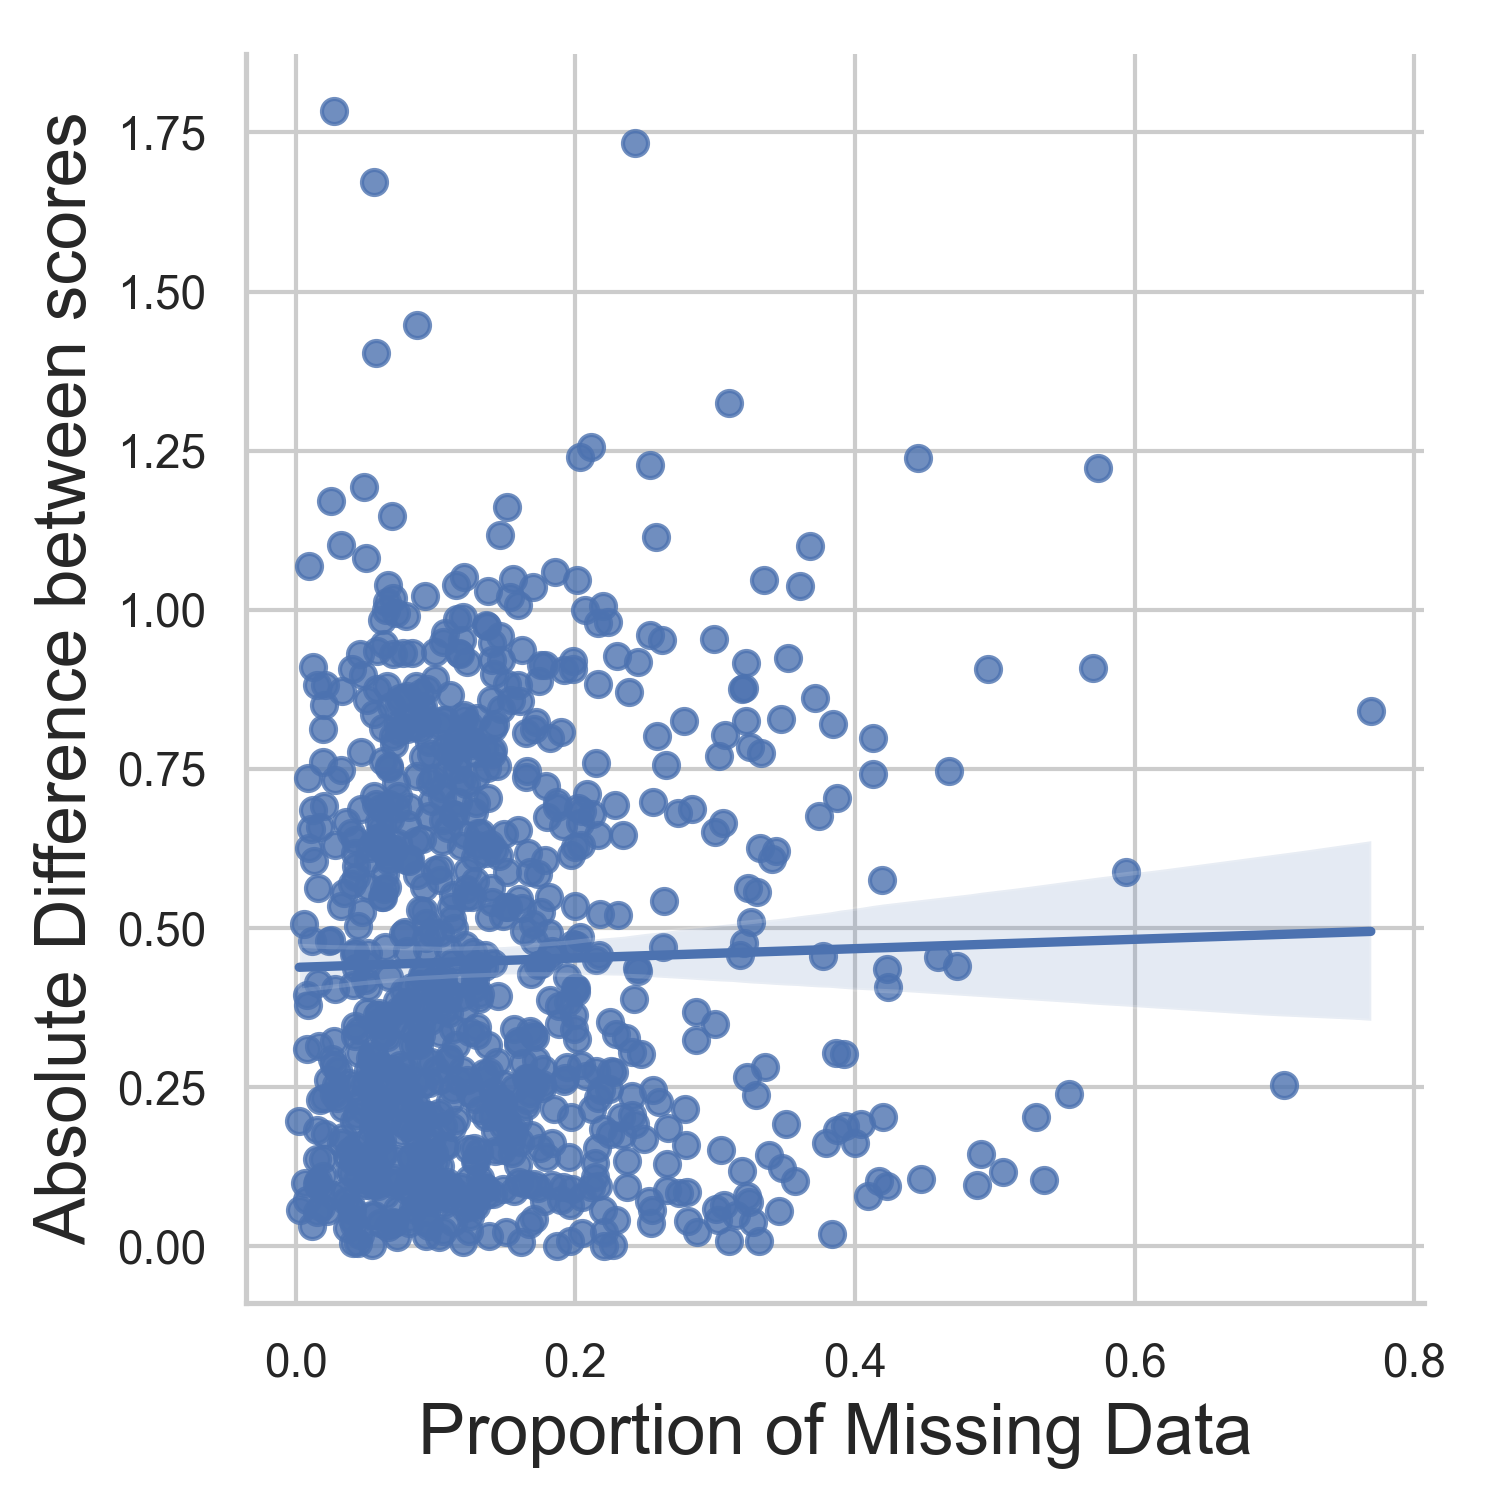
\includegraphics[width=\textwidth]{Graphs/missingvsdiff7}
            \caption{Proportion of missing votes and difference in scores EP7}
            \label{fig:missingscatter7}
        \end{subfigure}
        \hfill
        \begin{subfigure}[b]{0.48\textwidth}
            \centering
            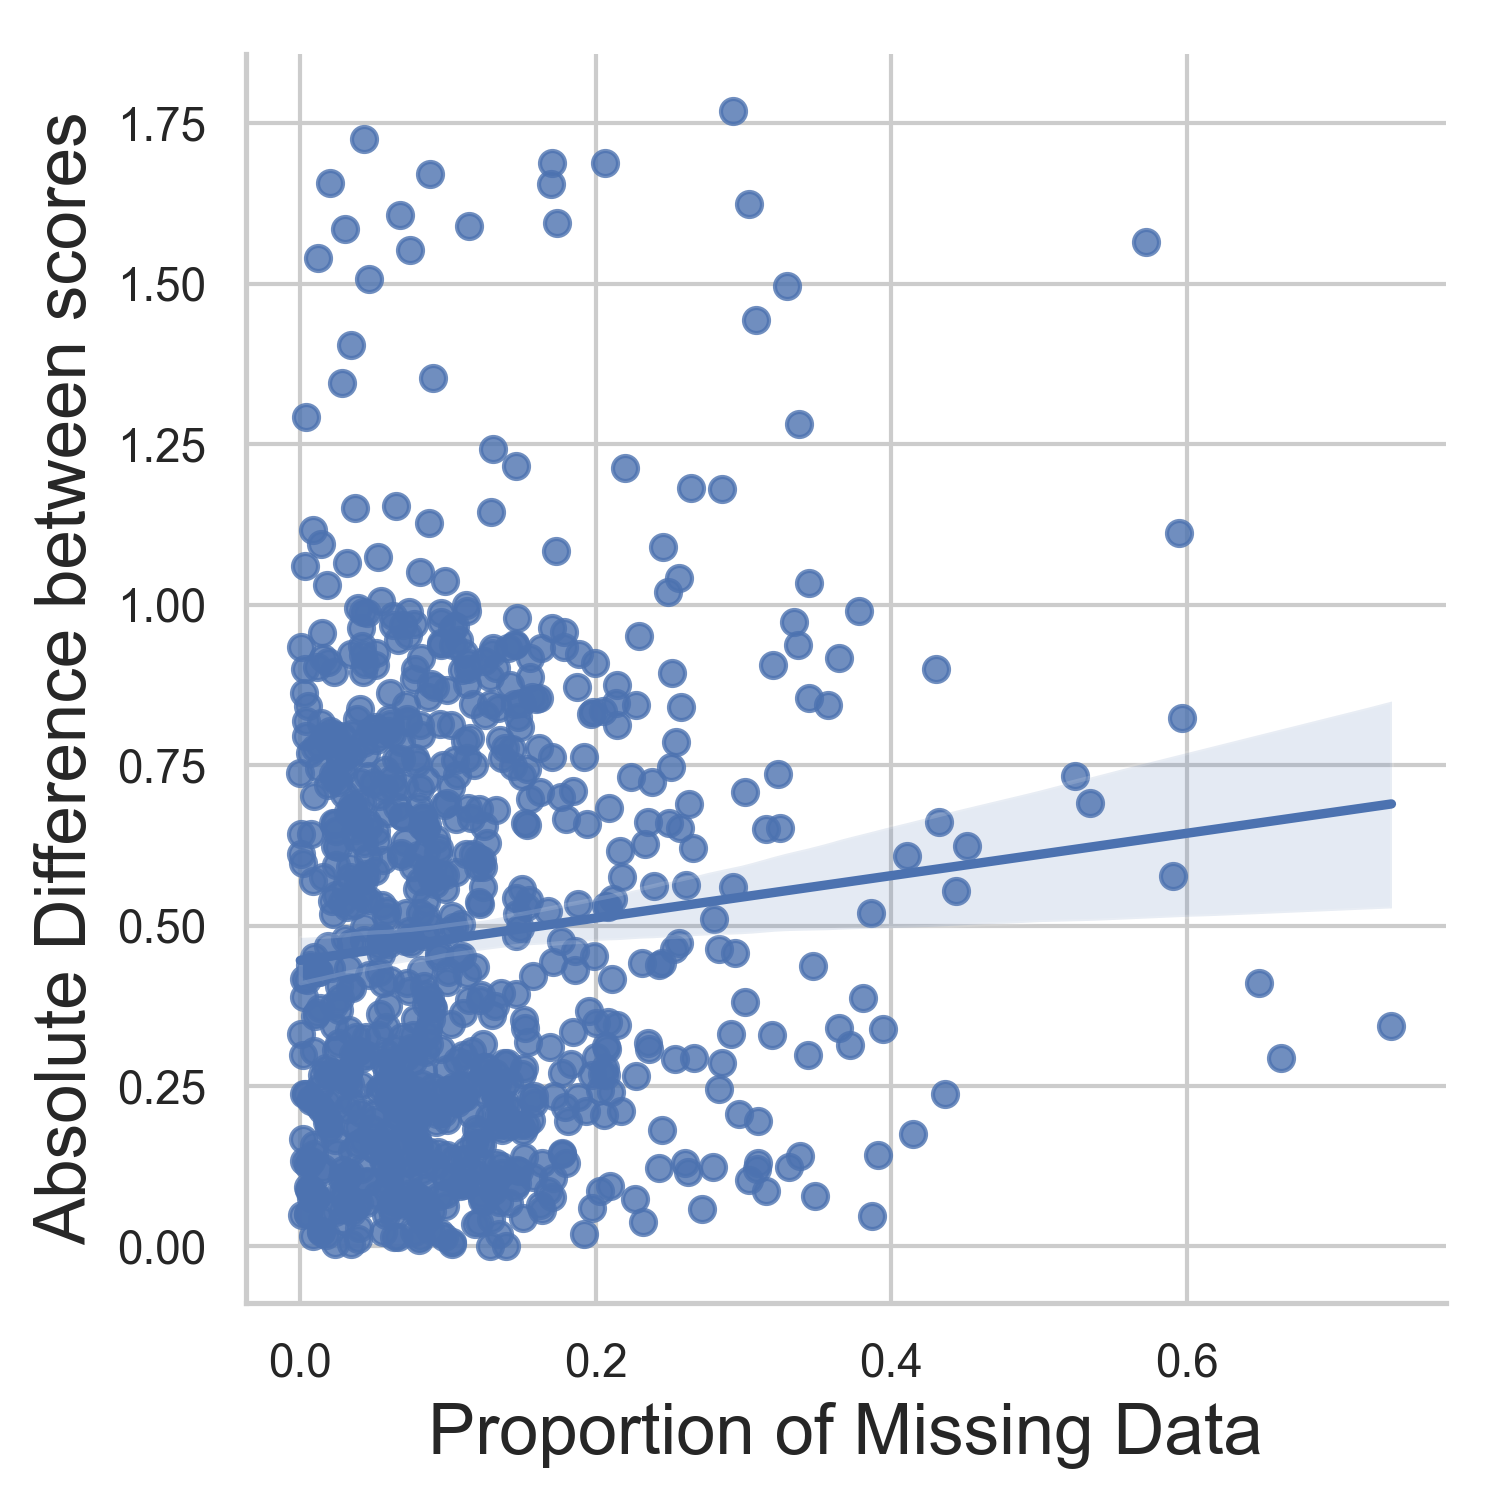
\includegraphics[width=\textwidth]{Graphs/missingvsdiff8}
            \caption{Proportion of missing votes and difference in scores EP7}
            \label{fig:missingscatter8}
        \end{subfigure}
        \caption{Scatter plots of proportion of missing votes and absolute differences in scores}
        \label{fig:missingscatters}
    \end{figure}

    \subsection{Investigation of diverging results.}\label{subsec:investigation-of-diverging-results.}
    In order to investigate the reason for the difference, we again turned to the methodology of Kosuke, Imai and
    Lo. In their paper, they prove that the difference in ideal point estimations is directly correlated with the
    amount of missing data, i.e.\ the more votes missing, the higher the probability of the emIRT algorithm to differ
    from the W-NOMINATE estimate.

    In our case, we were not able to verify this claim.
    There was no clear correlation between the amount of missing
    votes and the absolute difference between the results.
    Not being able to quickly verify the issue, we decided to
    examine the problem in more detail.

    We created scatter plots of the diverging results for each EPG individually.
    This action allowed for more
    insight into the issue.
    From the three biggest groups, 2 were almost perfectly aligned - ALDE and S\&D had high
    Pearson correlation coefficients and were situated in similar positions using both methods. But the biggest
    group in the European Parliament - EPP had the most diverging results. While W-NOMINATE places it firmly in the
    center of the spectrum, in range of [-0.1,0,1], emIRT placed it significantly more on the right, with a wider range
    of [0.45,0.95]. Apart from this politcal group, the smaller, more radical ones had low correlations as well.
    emIRT authors did find the more radical legislators usually have a bigger difference than the centrist ones
    between the algorithms, so that is to be expected. However, the differences are greater tham what their research
    would lead us to expect.
    As of the moment of writing this dissertation, we were not able to identify the reason behind
    this behaviour.
    Further research is necessary in order to explain this behaviour within this particular dataset.


    \section{Initialization research}

    In order to better understand the software we are using to estimate the ideal points, we decided to conduct
    research on the mechanisms of initializing the algorithms.
    With this additional context, we aimed to see the
    impact of different initialization methods on the results, and possibly explain the discrepancy found in the
    results of the two methods.

    \subsection{Obtaining the starting values of W-NOMINATE}\label{subsec:obtaining-the-starting-values-of-w-nominate}
    To understand the initialization procedure of W-NOMINATE, review of the original Fortran implementation of the
    software was necessary.
    As explained in detail in Chapter 4, W-NOMINATE obtains its' starting points by
    calculating an agreement matrix, calculating the mean distances
    between legislators' votes on every piece of legislation in the dataset. The eigenvectors of the matrix are then
    extracted to provide an approximation of the ideal points.

    \subsection{Initializing emIRT with W-NOMINATE starts}\label{subsec:initializing-emirt-with-w-nominate-starts}
    Our goal was initializing emIRT with starting points of W-NOMINATE and vice versa. Comparing the results of
    those operations with the original results would help us explain if and how the initialization process impacts
    the algorithm.

    In order to obtain the starting points of W-NOMINATE to initialize emIRT with, we reverse engineered the
    original Fortran implementation and translated it into \texttt{R}.
    To optimize the original algorithm, which used
    numerous nested for loops and linear operations, we opted for a more modern approach utilizing \texttt{R}'s
    vectorized operations.

    After obtaining the eigenvectors to use as starts in emIRT, and following the default method of setting the
    \(\alpha\) (difficulty) and \(\beta_j\)
    (discrimination) parameters to zero, we initialized the algorithm with the same settings as before. The software
    was able to produce results with the modified initialization method.

    We have also made attempts to use emIRT's initialization method in W-NOMINATE. This required editing the Fortran
    source code of the package.
    changing the method of initialization from the eigenvectors to starts obtained from a
    normal distribution and recompiling it with the new settings.
    Unfortunately, we were unable to successfully
    estimate ideal points using this method, due to problems with the technical implementation.
    \begin{figure}[H]
        \centering
        \begin{subfigure}[b]{0.48\textwidth}
            \centering
            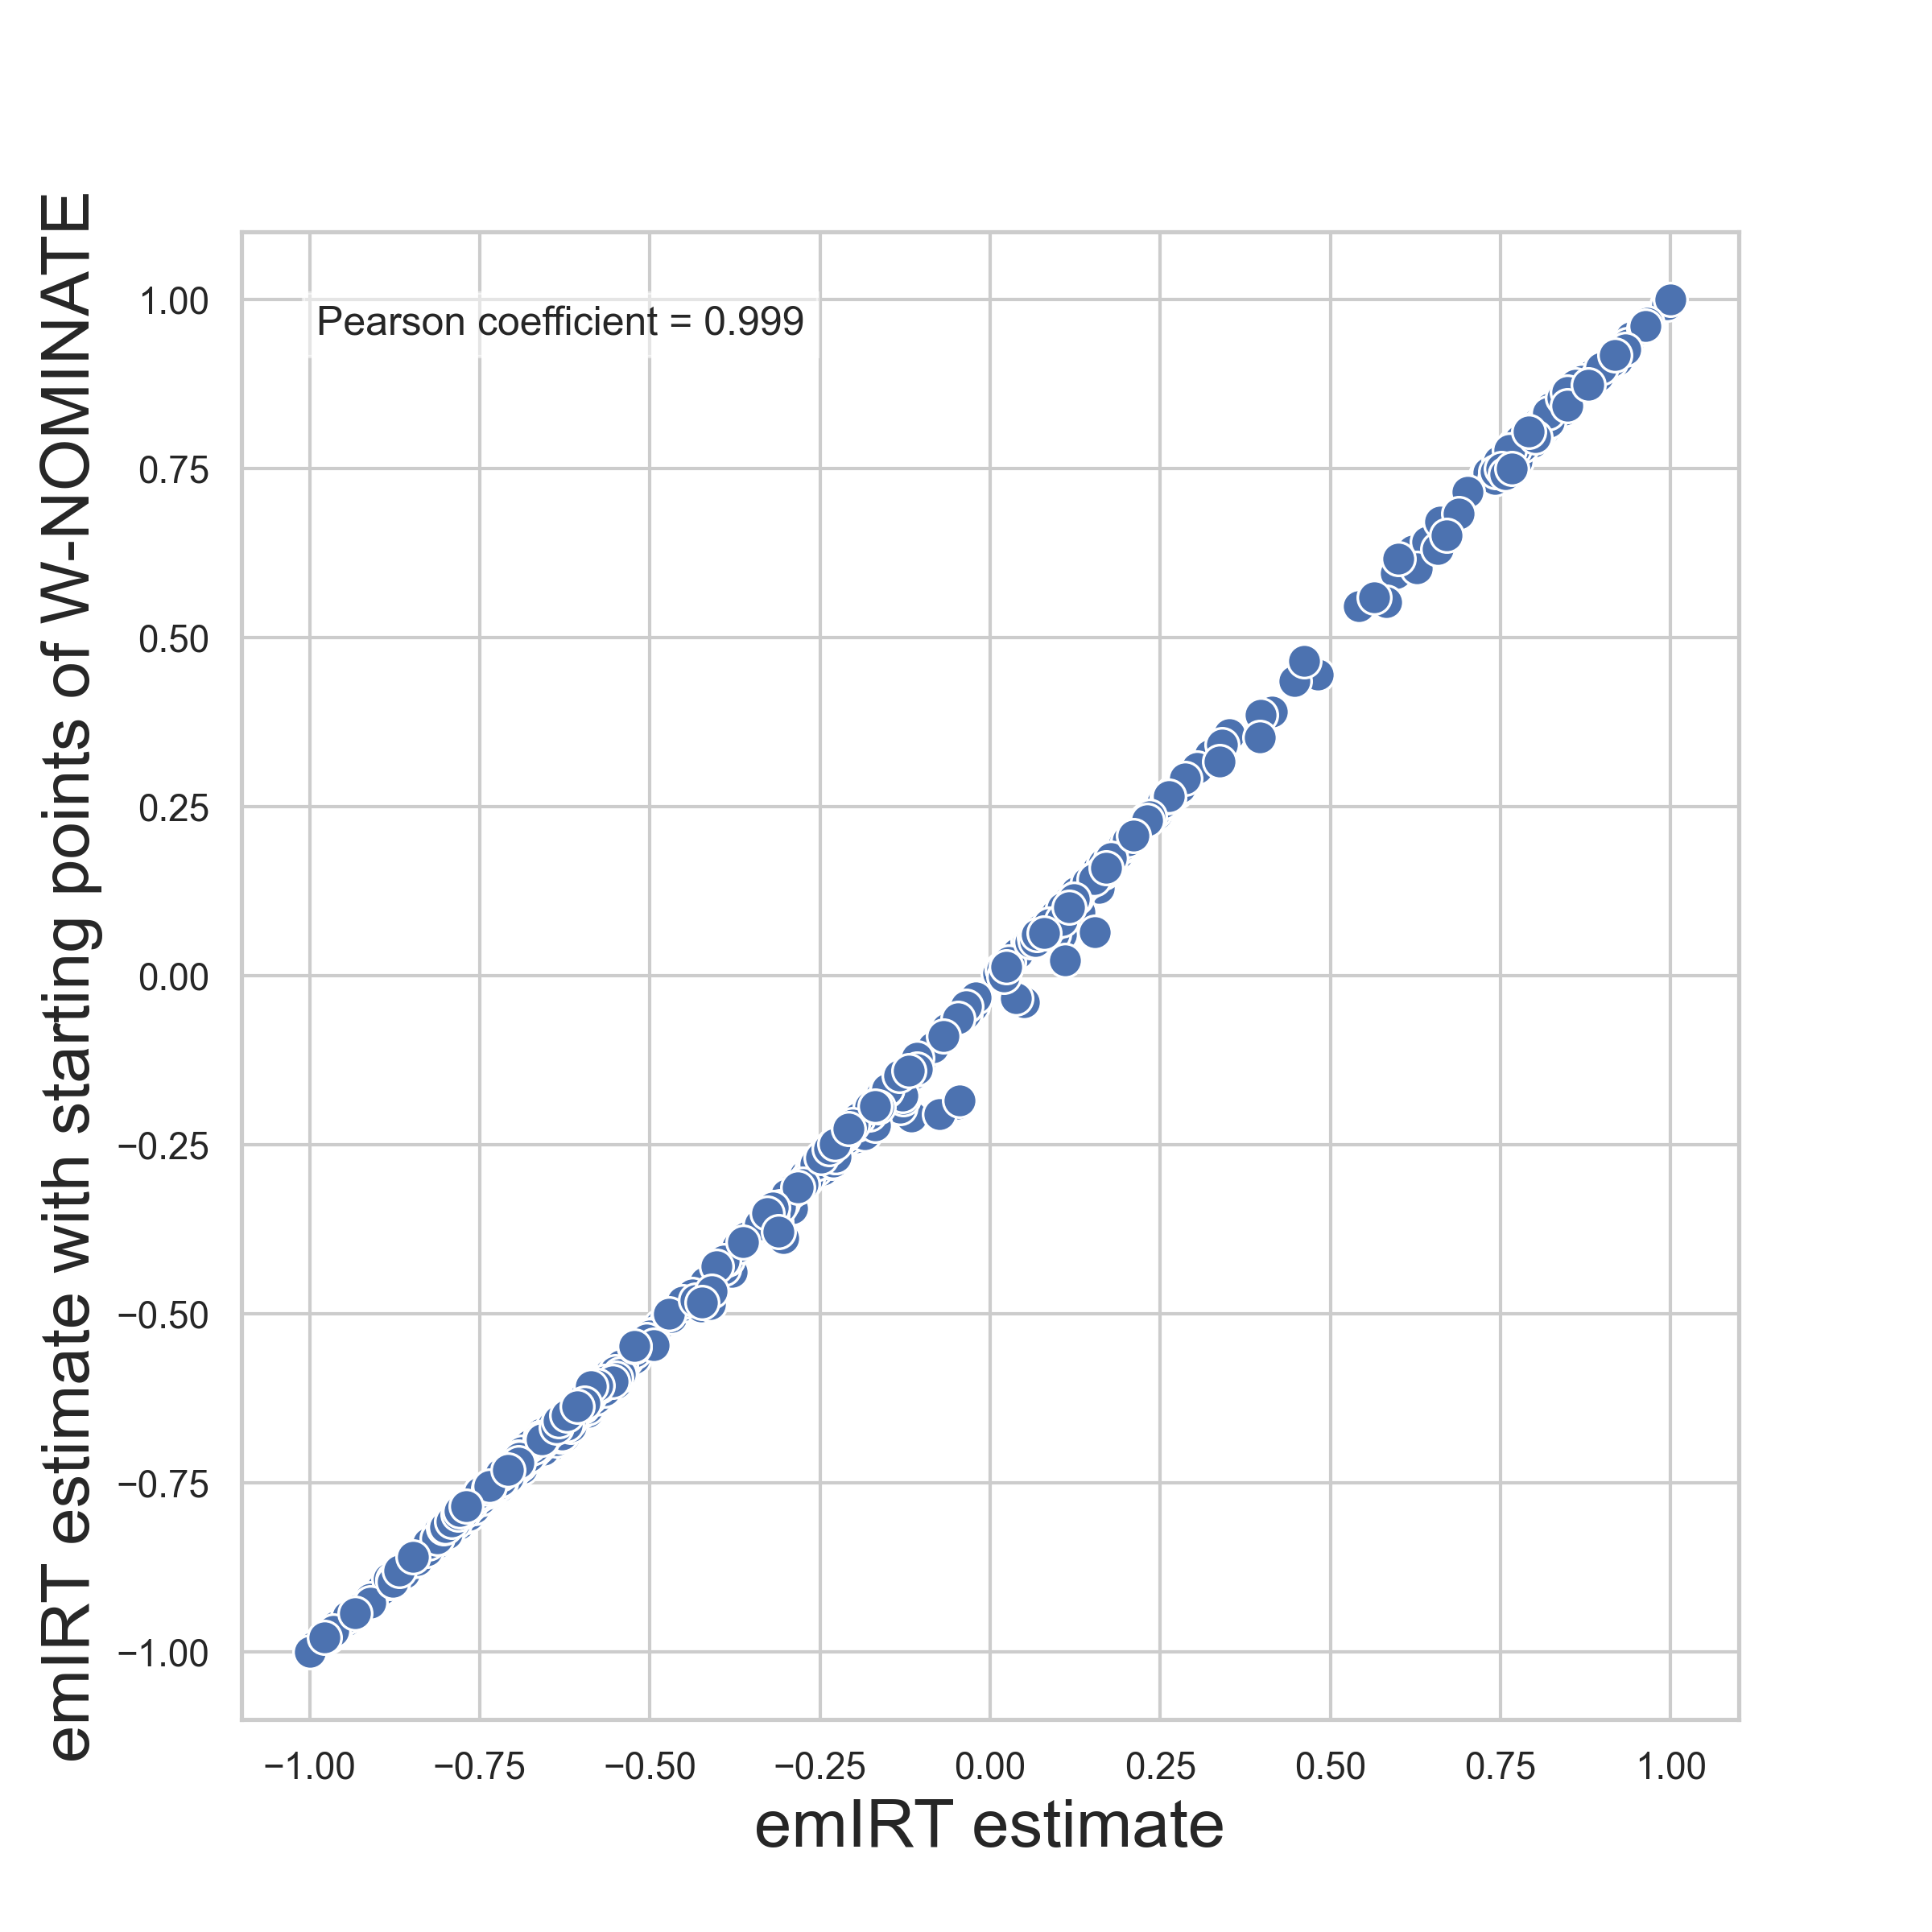
\includegraphics[width=\textwidth]{Graphs/ScatterEMEIGEN6}
            \caption{emIRT and emIRT with W-NOMINATE starts in EP6}
            \label{fig:EMEIGEN_SCATTER_6}
        \end{subfigure}
        \hfill
        \begin{subfigure}[b]{0.48\textwidth}
            \centering
            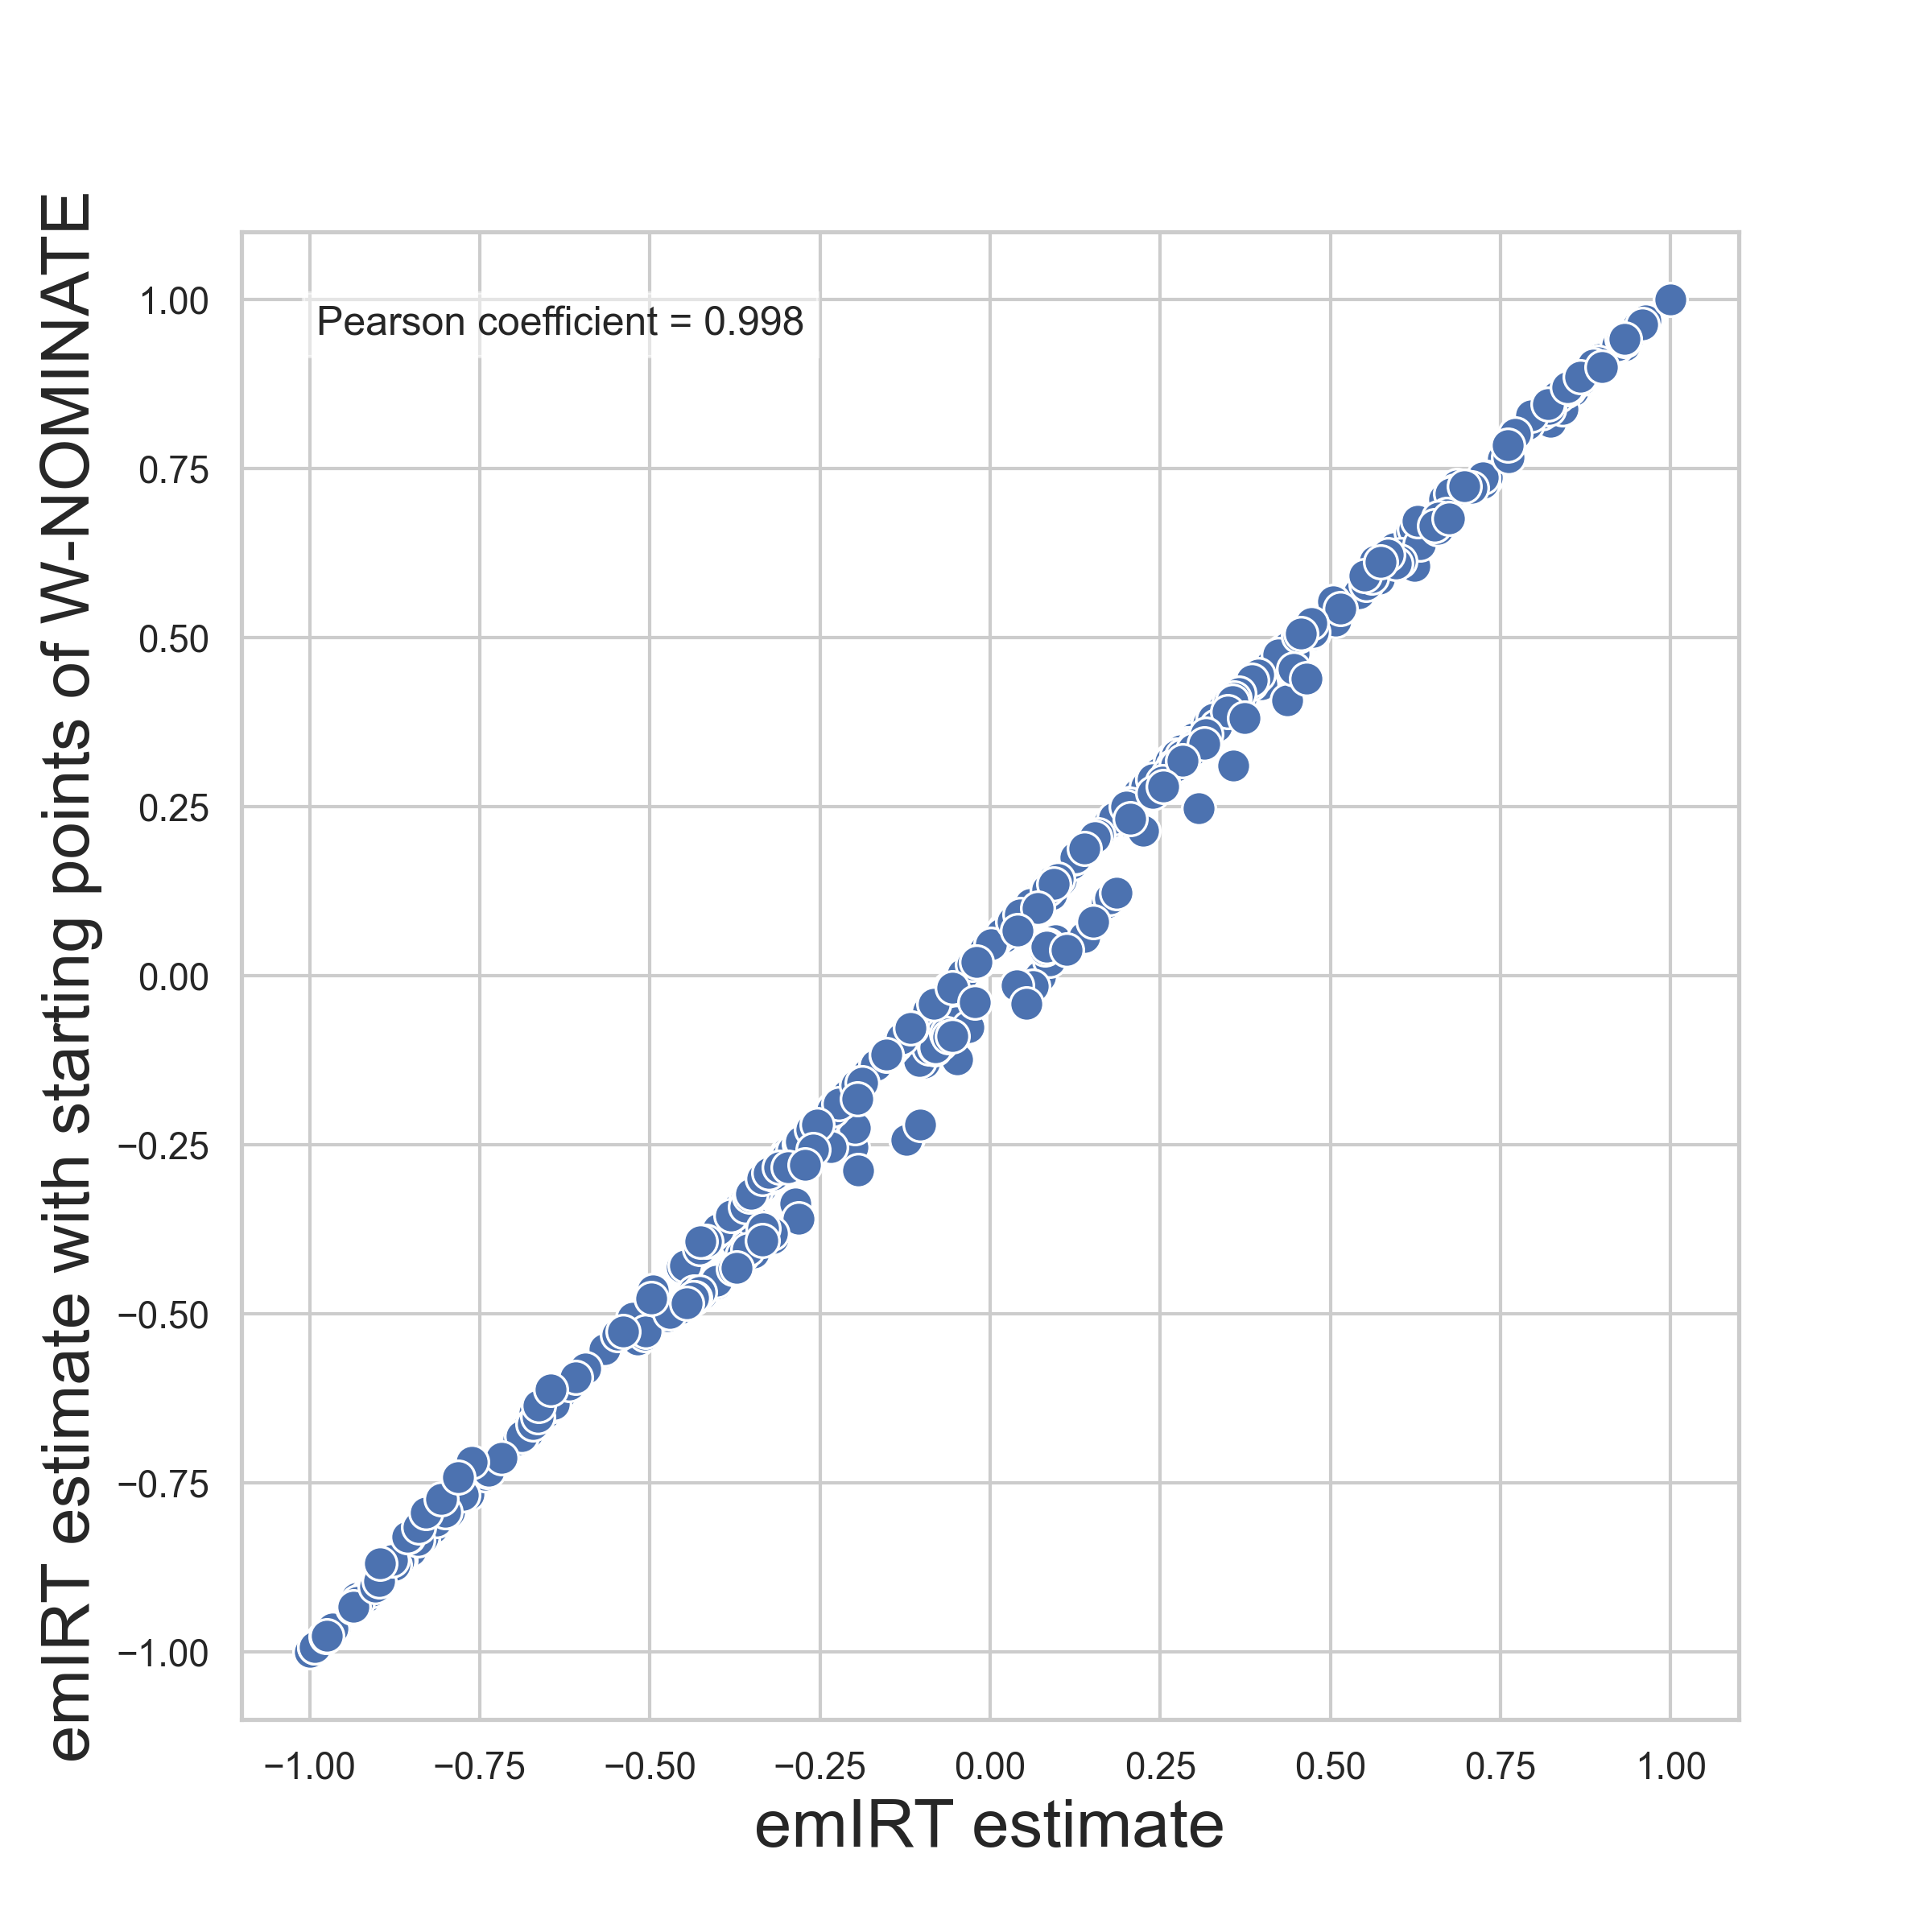
\includegraphics[width=\textwidth]{Graphs/ScatterEMEIGEN9}
            \caption{emIRT and emIRT with W-NOMINATE starts in EP9}
            \label{fig:EMEIGEN_SCATTER_9}
        \end{subfigure}
        \caption{Scatter plots of emIRT and emIRT with W-NOMINATE starts estimations of ideal points in EP6 and EP9}
        \label{fig:EMEIGEN_SCATTER_6_9}
    \end{figure}
    \begin{figure}[H]
        \centering
        \begin{subfigure}[b]{0.48\textwidth}
            \centering
            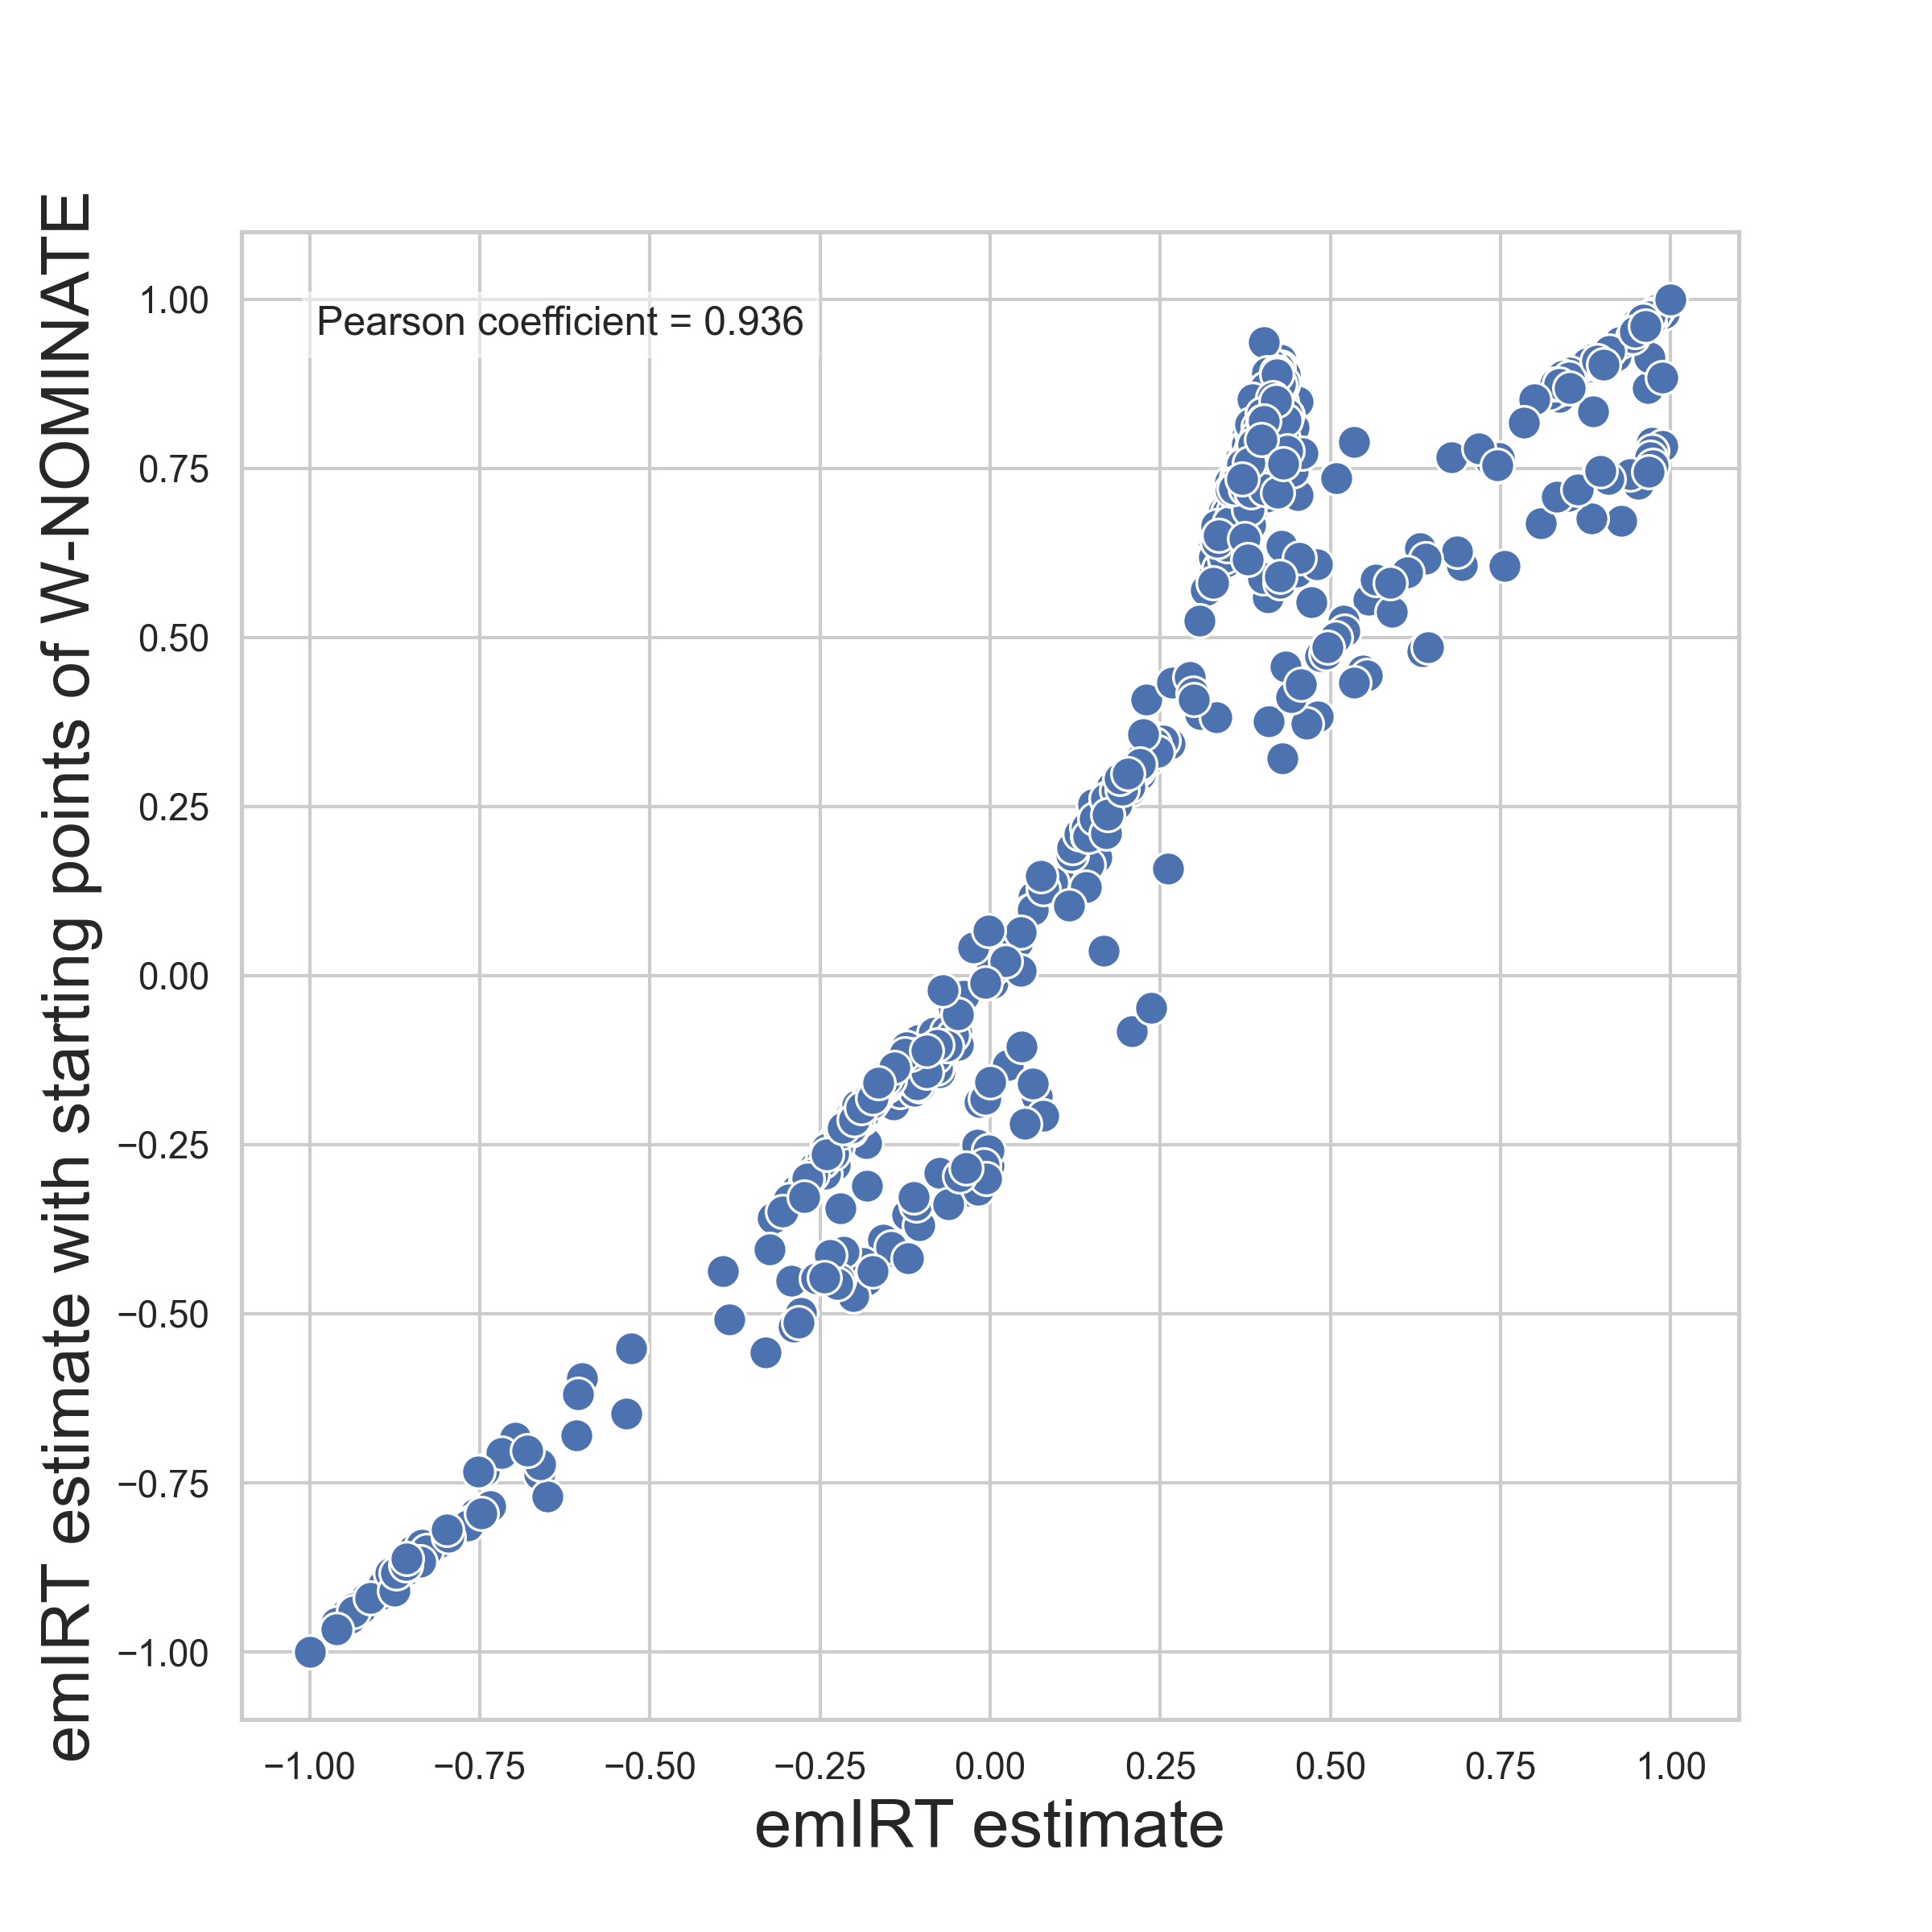
\includegraphics[width=\textwidth]{Graphs/ScatterEMEIGEN7}
            \caption{emIRT and emIRT with W-NOMINATE starts in EP7}
            \label{fig:EMEIGEN_SCATTER_7}
        \end{subfigure}
        \hfill
        \begin{subfigure}[b]{0.48\textwidth}
            \centering
            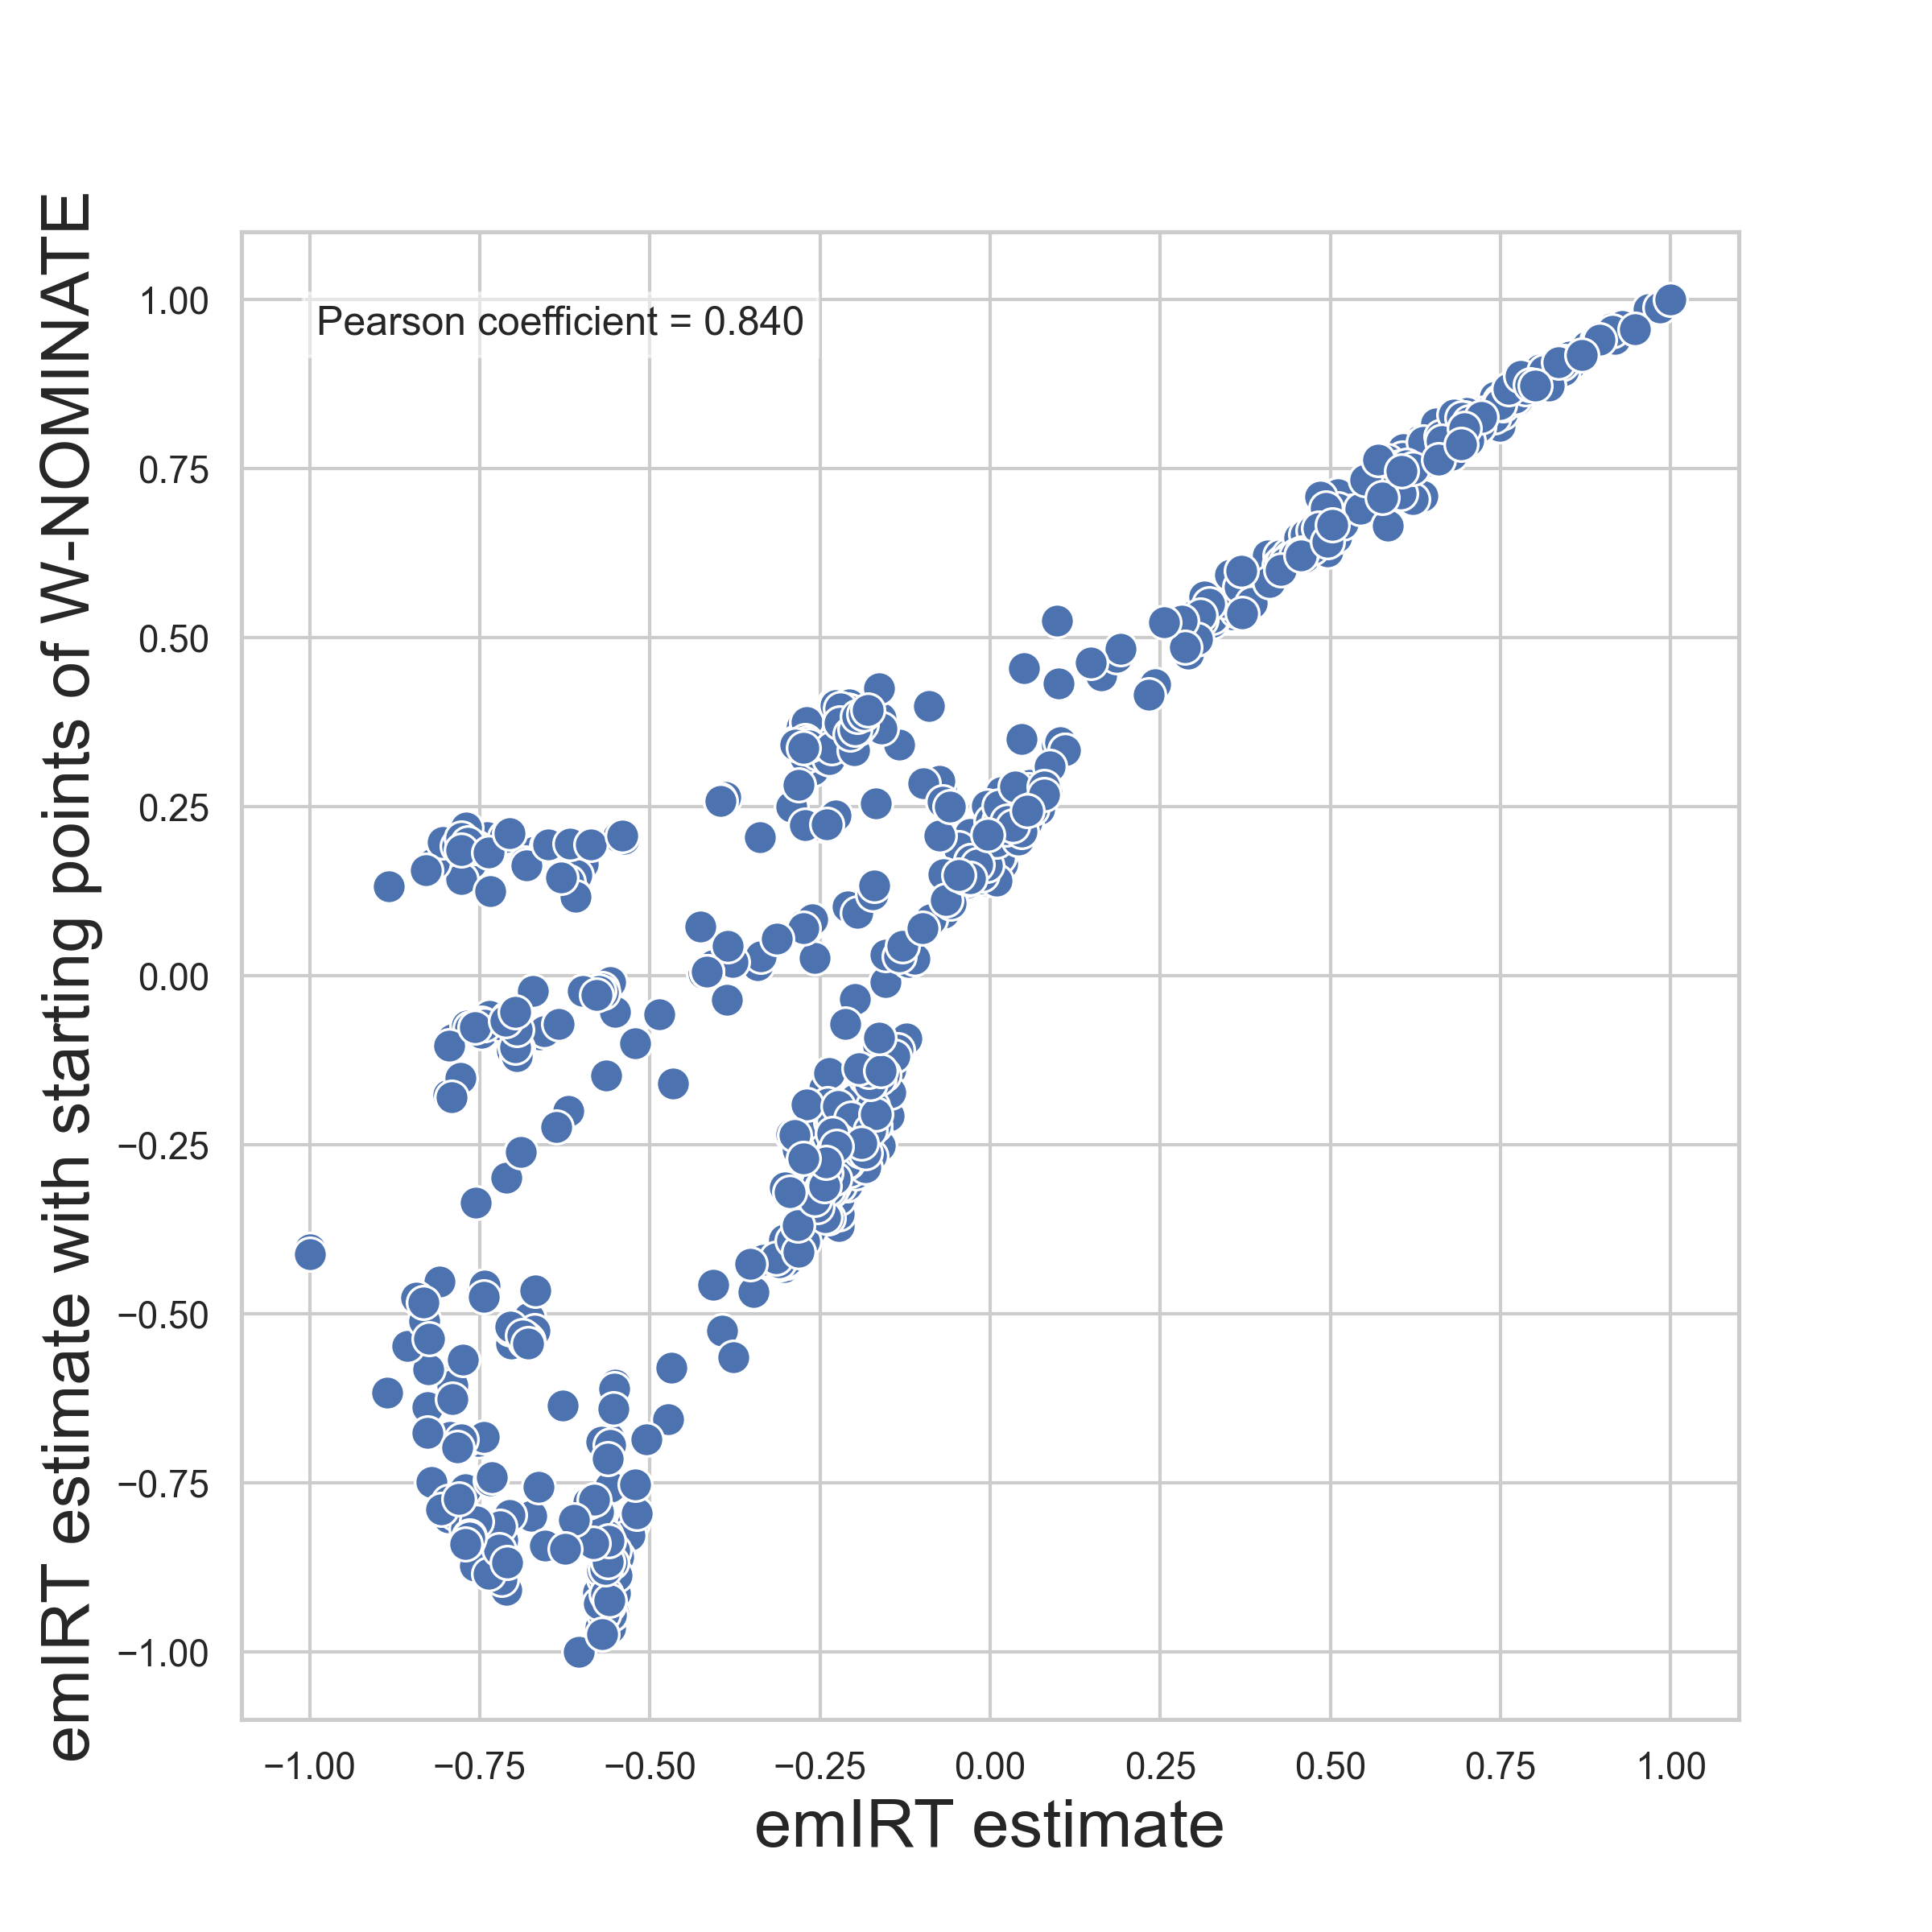
\includegraphics[width=\textwidth]{Graphs/ScatterEMEIGEN8}
            \caption{emIRT and emIRT with W-NOMINATE starts in EP8}
            \label{fig:EMEIGEN_SCATTER_8}
        \end{subfigure}
        \caption{Scatter plots of emIRT and emIRT with W-NOMINATE starts estimations of ideal points in EP7 and EP8}
        \label{fig:EMEIGEN_SCATTER_7_8}
    \end{figure}
    \begin{figure}[H]
        \centering
        \begin{subfigure}[b]{0.48\textwidth}
            \centering
            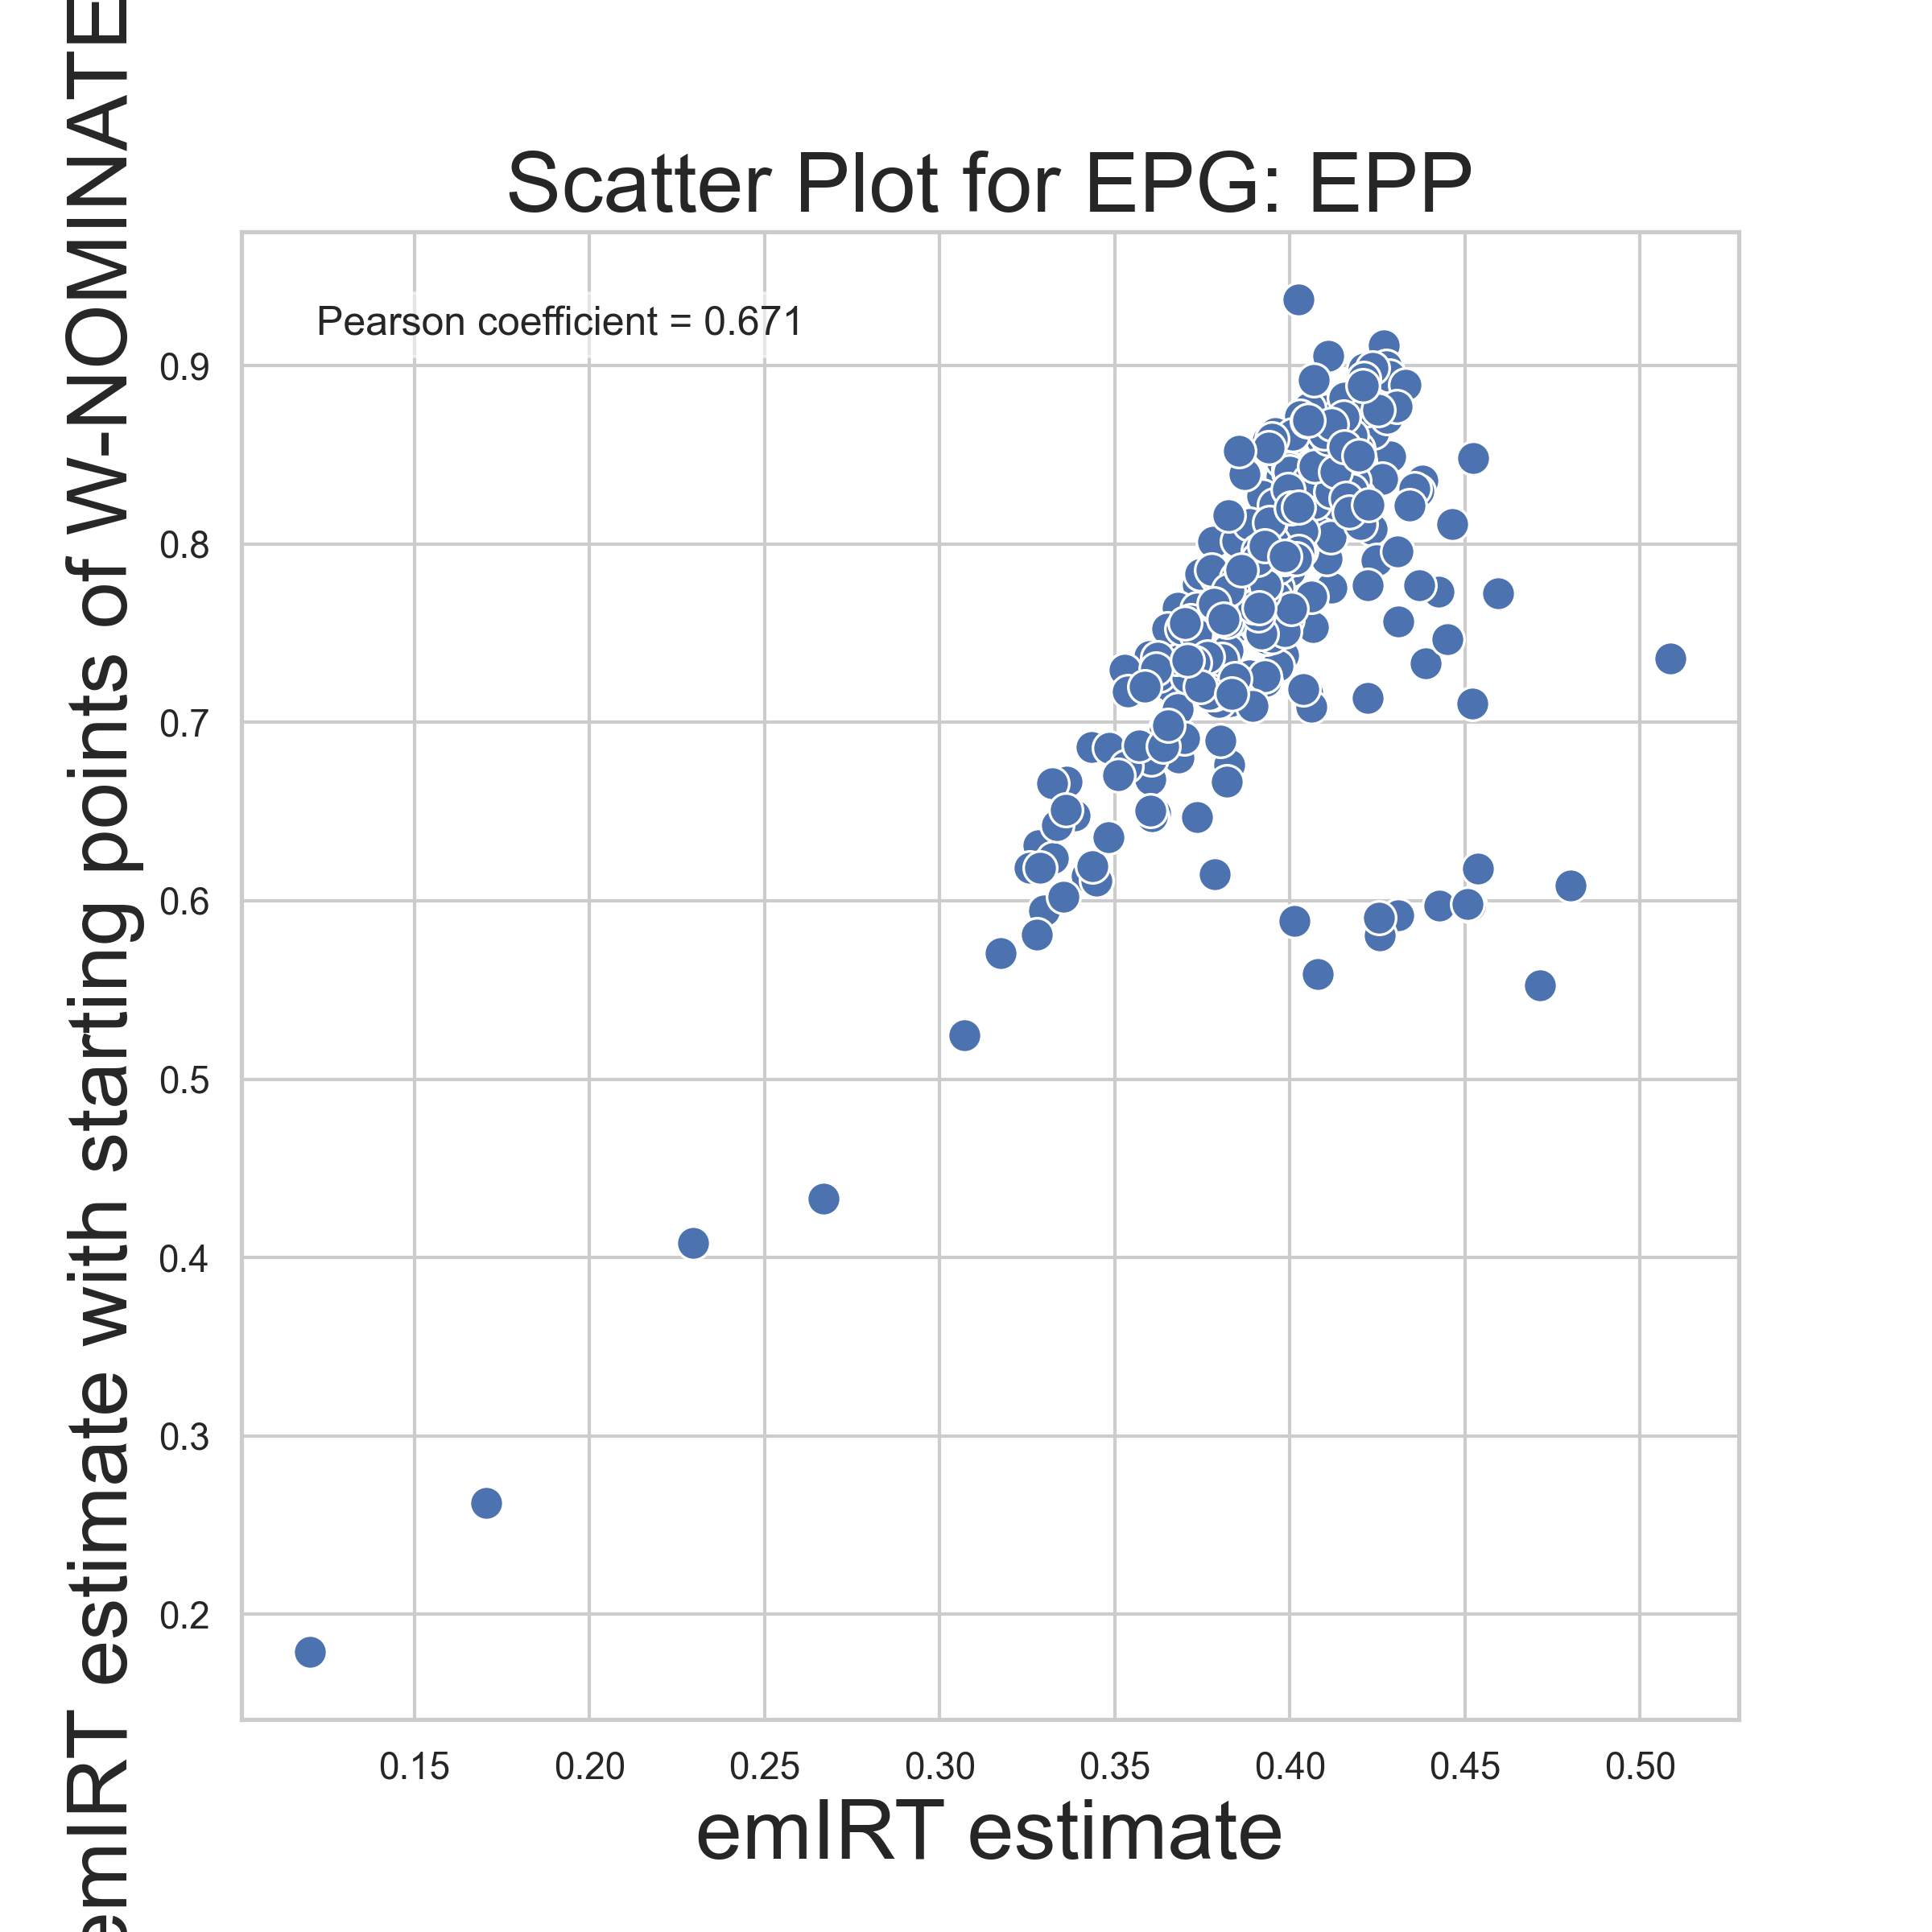
\includegraphics[width=\textwidth]{Graphs/ScatterEMEIGEN_7_EPG_EPP}
            \caption{emIRT and emIRT with W-NOMINATE starts in EP7 (EPP)}
            \label{fig:EMEIGEN_SCATTER_7EPP}
        \end{subfigure}
        \hfill
        \begin{subfigure}[b]{0.48\textwidth}
            \centering
            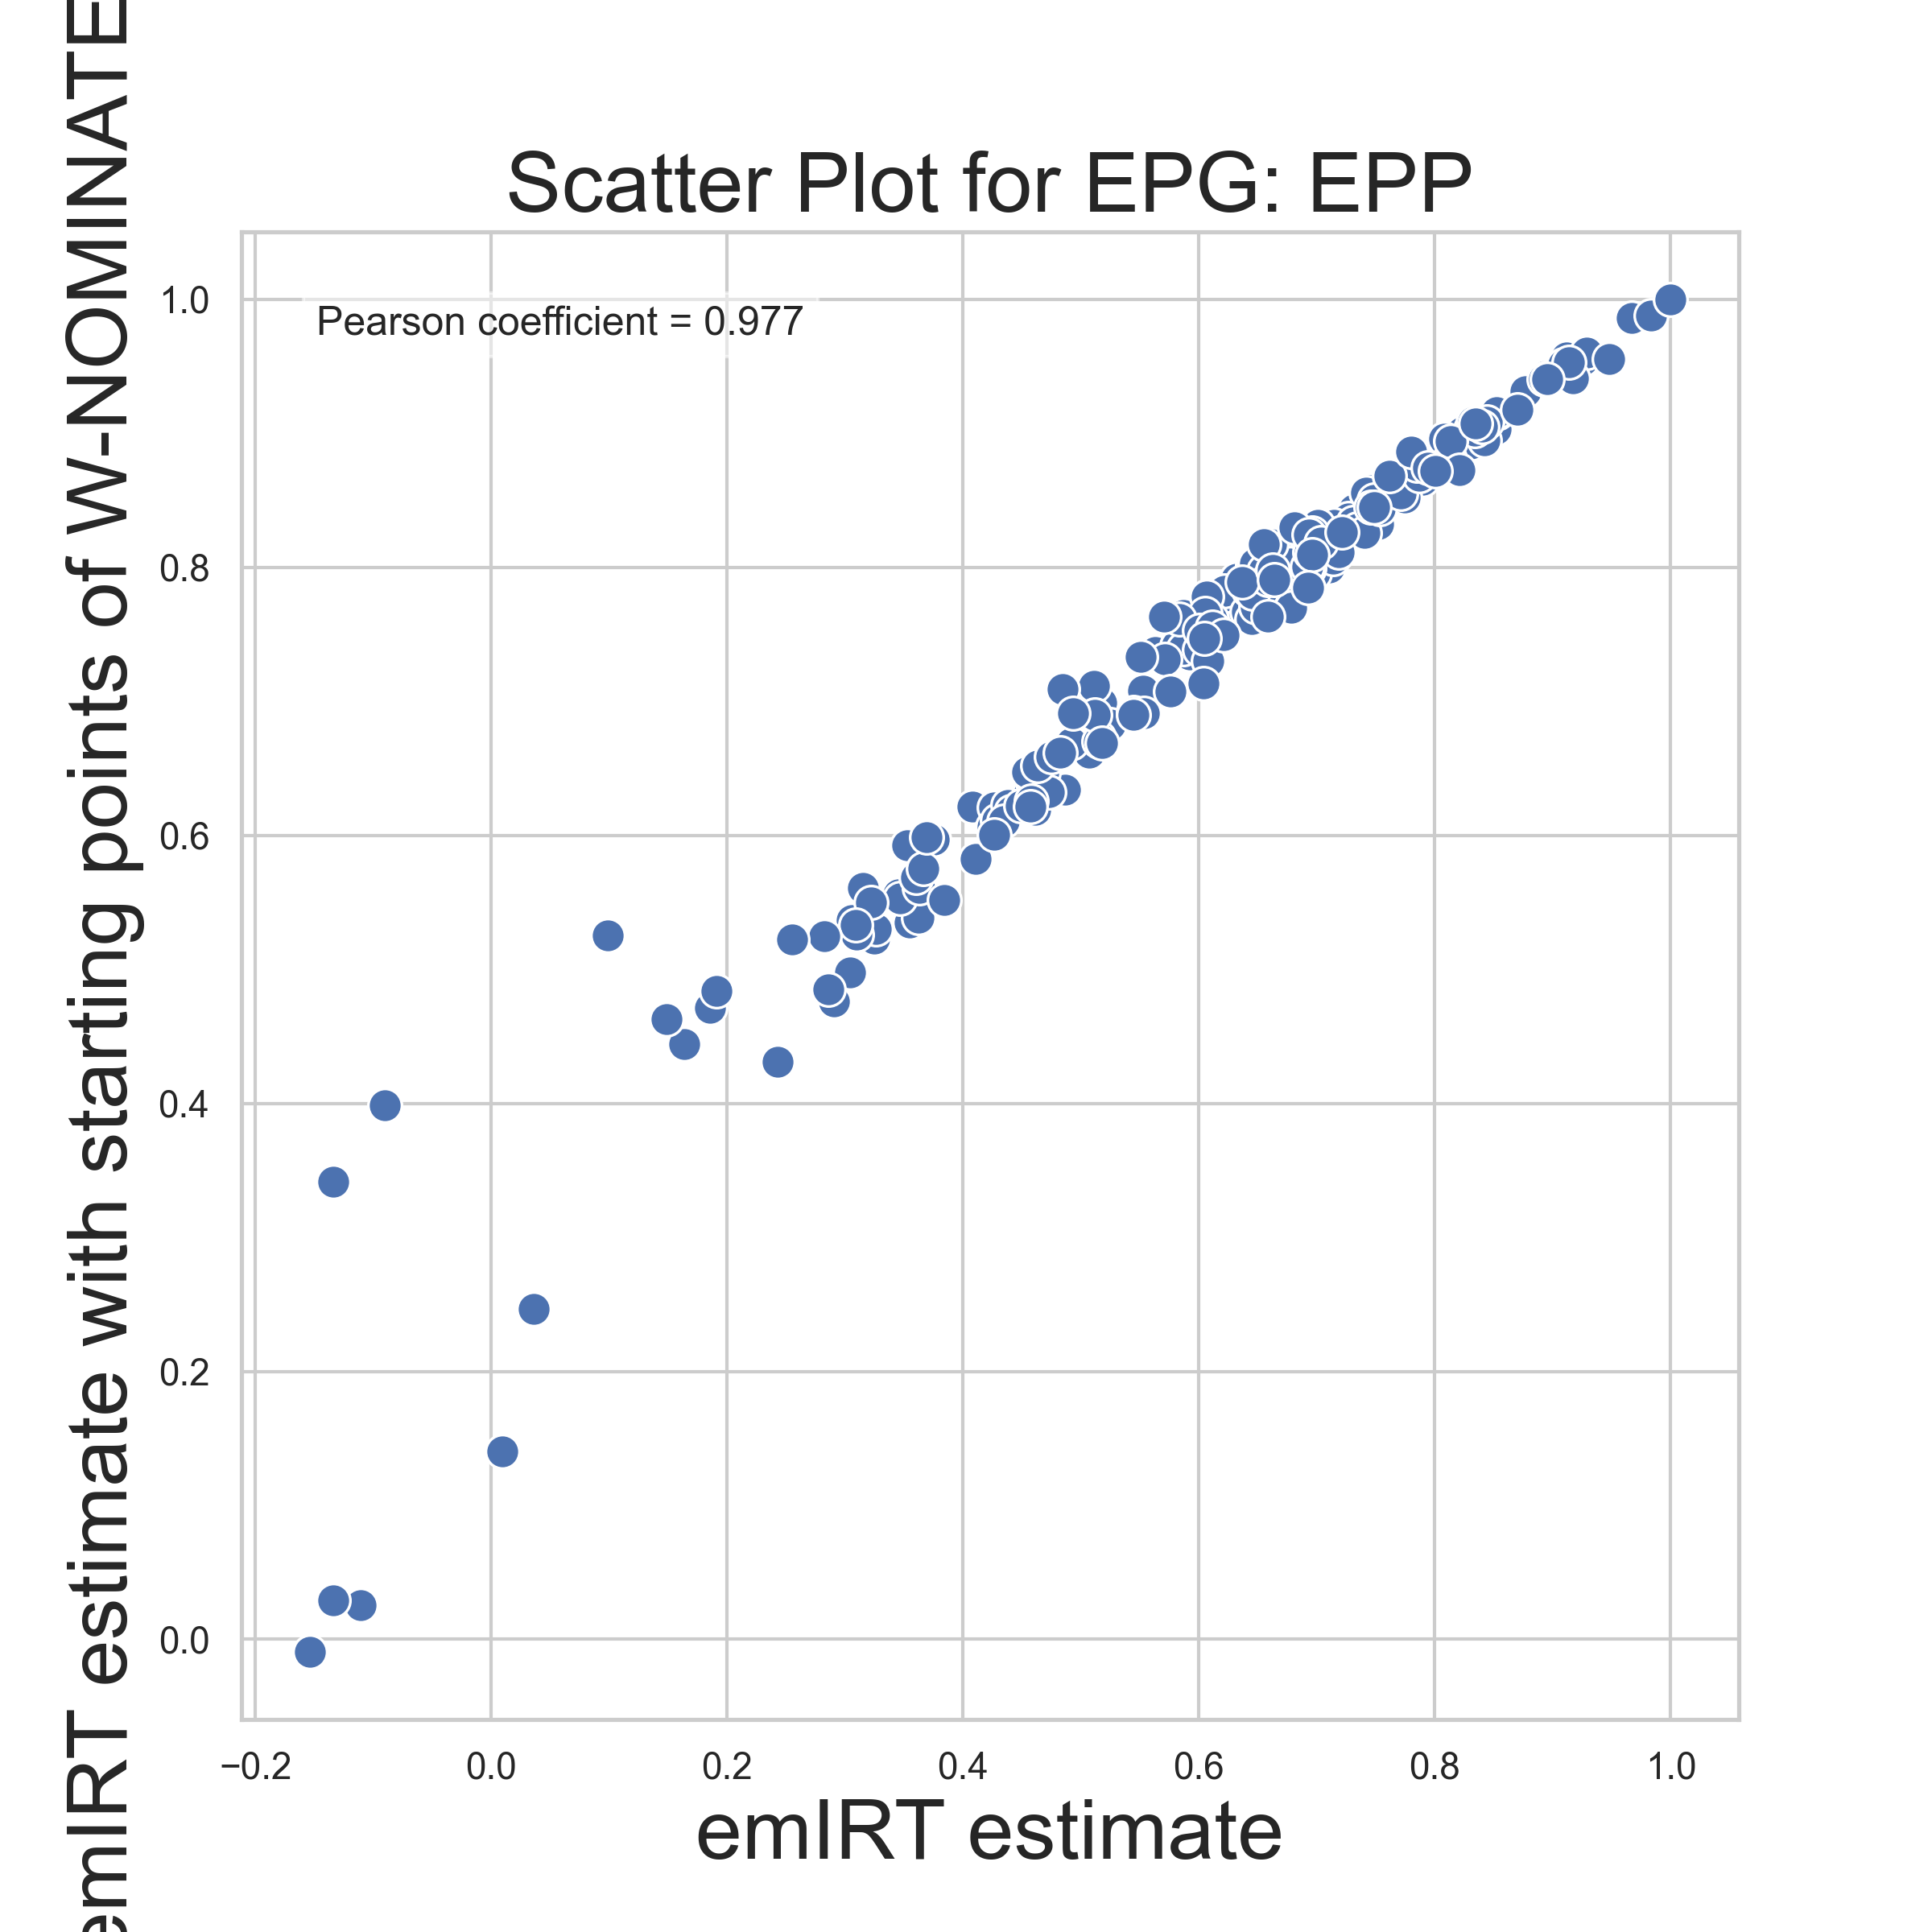
\includegraphics[width=\textwidth]{Graphs/ScatterEMEIGEN_8_EPG_EPP}
            \caption{emIRT and emIRT with W-NOMINATE starts in EP8 (EPP)}
            \label{fig:EMEIGEN_SCATTER_8EPP}
        \end{subfigure}
        \caption
        {Scatter plots of emIRT and emIRT with W-NOMINATE starts estimations of ideal points in EP7 and EP8 for EPP}
        \label{fig:EMEIGEN_SCATTER_7_8EPP}
    \end{figure}
    \begin{figure}[H]
        \centering
        \begin{subfigure}[b]{0.48\textwidth}
            \centering
            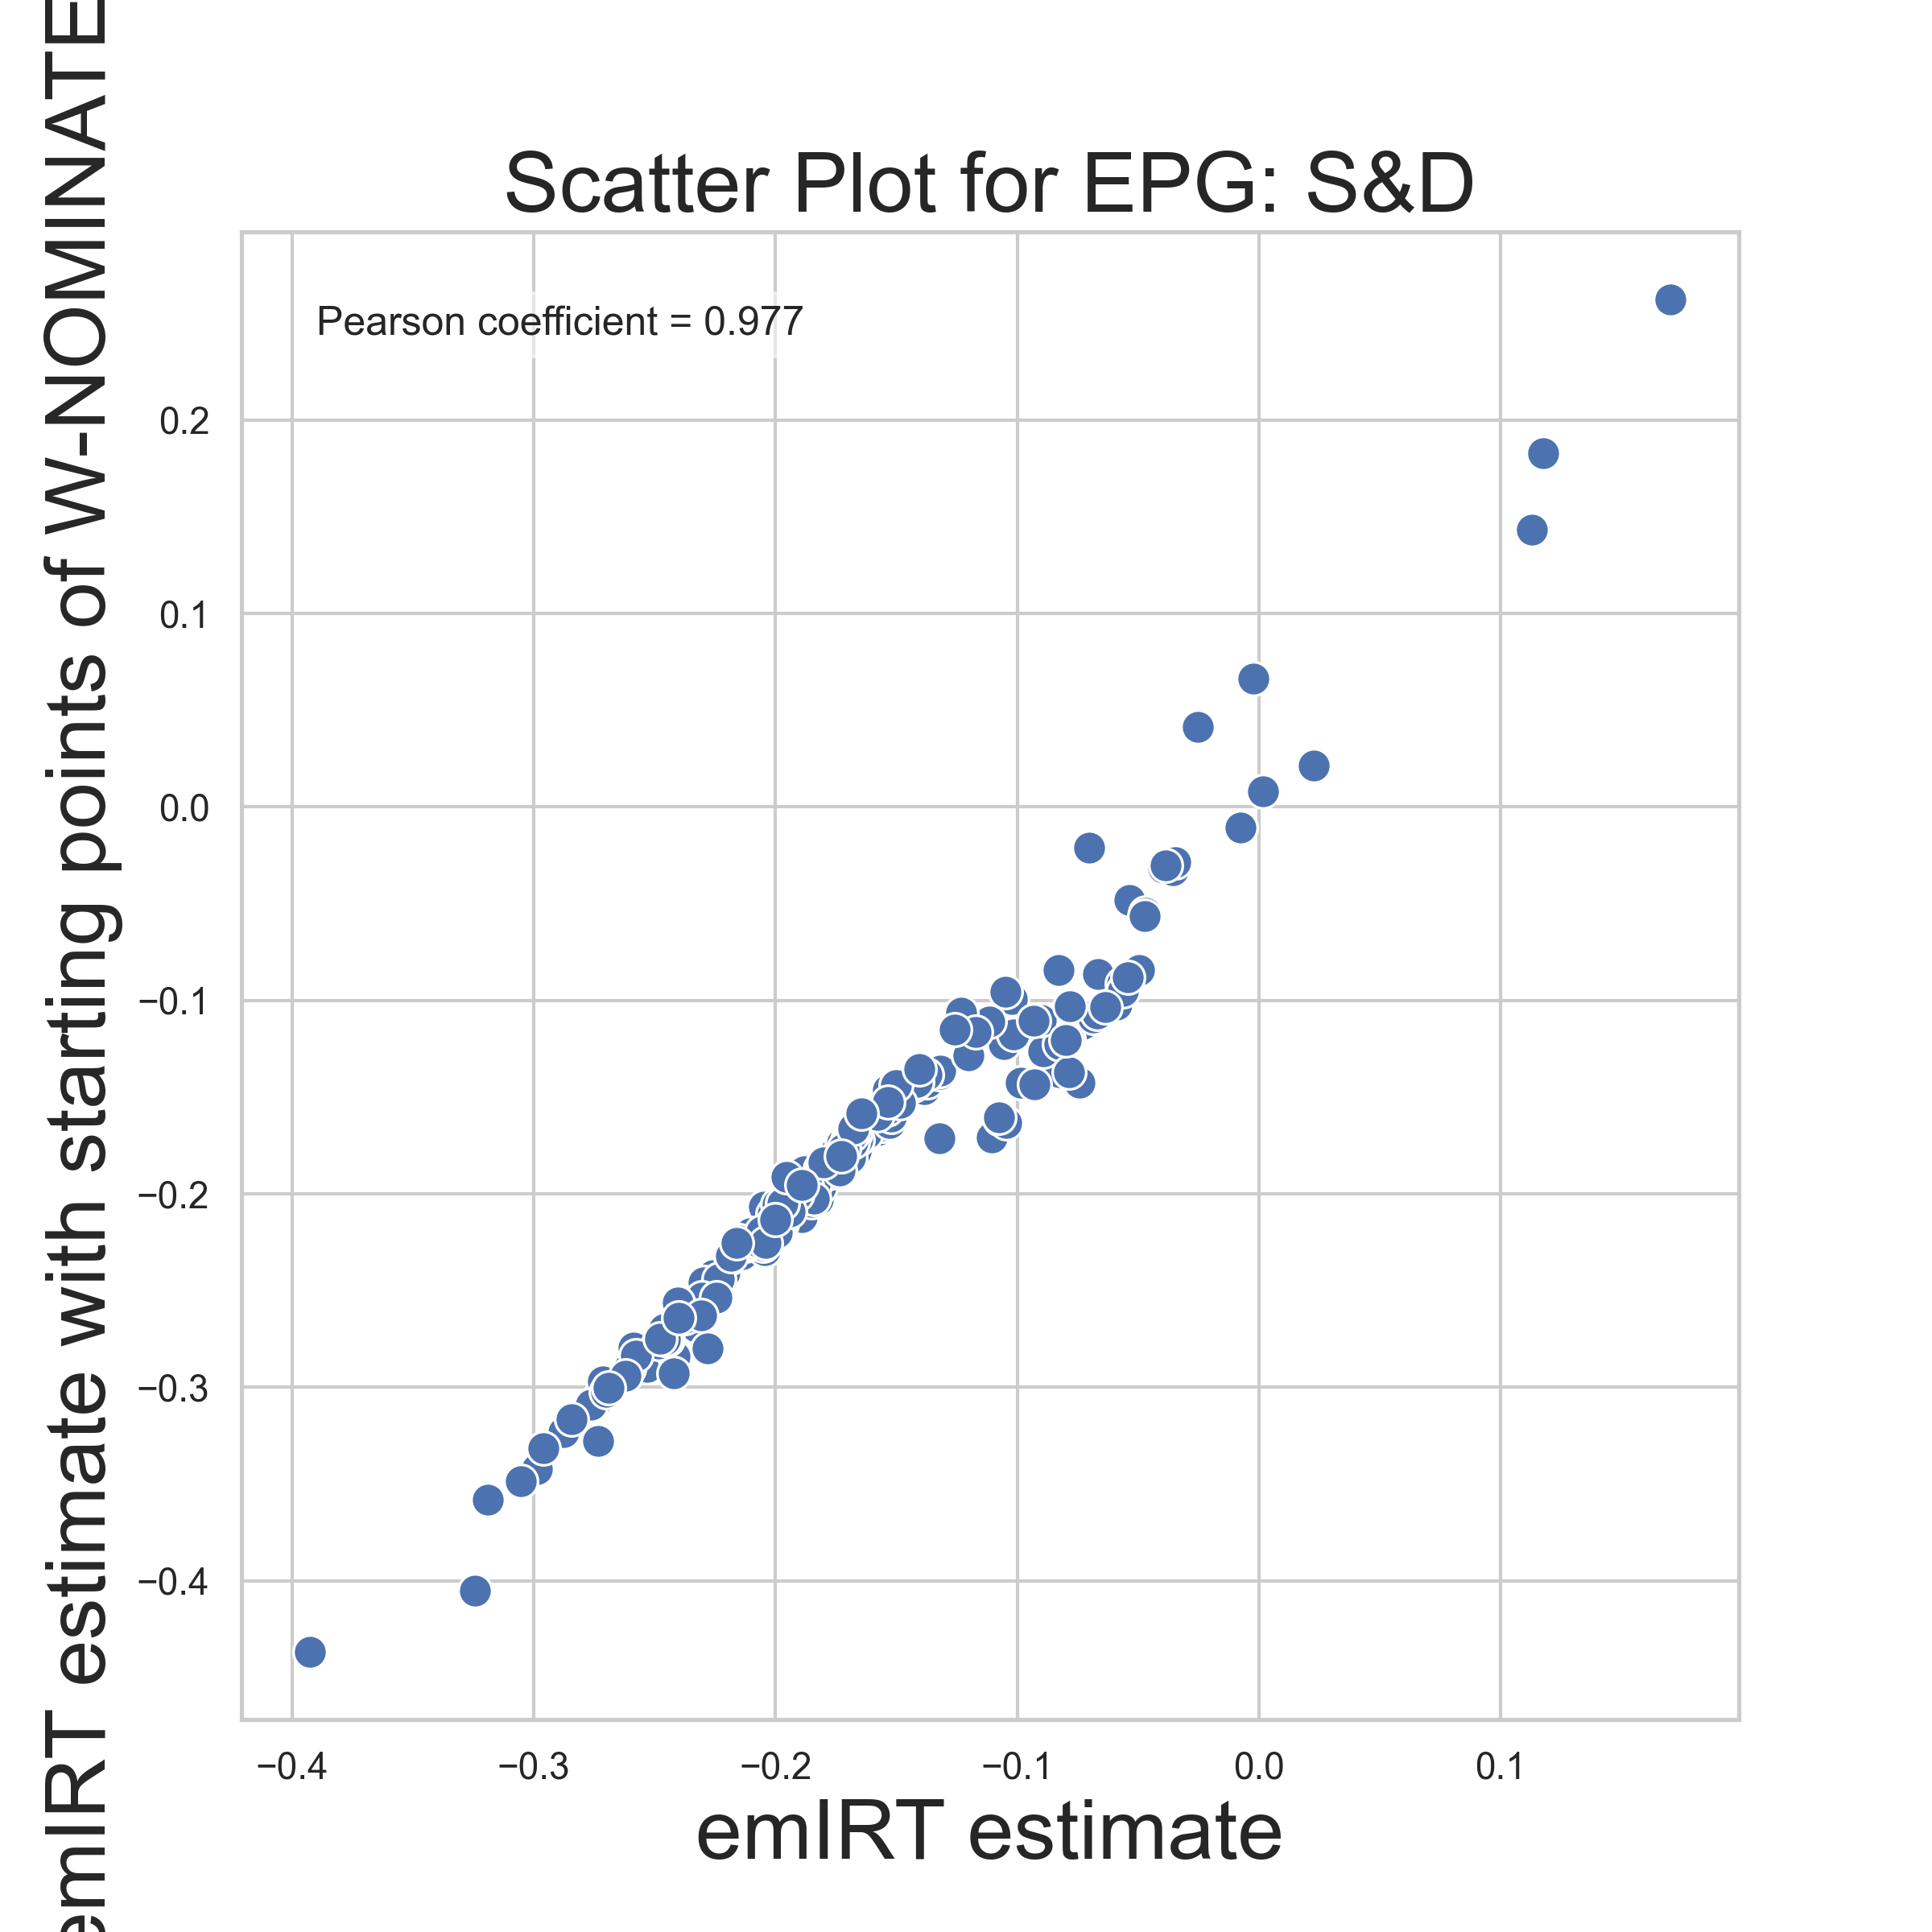
\includegraphics[width=\textwidth]{Graphs/ScatterEMEIGEN_7_EPG_S&D}
            \caption{emIRT and emIRT with W-NOMINATE starts in EP7 (S\&D)}
            \label{fig:EMEIGEN_SCATTER_7SD}
        \end{subfigure}
        \hfill
        \begin{subfigure}[b]{0.48\textwidth}
            \centering
            \includegraphics[width=\textwidth]{Graphs/ScatterEMEIGEN_8_EPG_Greens–EFA}
            \caption{emIRT and emIRT with W-NOMINATE starts in EP8 (Greens)}
            \label{fig:EMEIGEN_SCATTER_8Grens}
        \end{subfigure}
        \caption
        {Scatter plots of emIRT and emIRT with W-NOMINATE starts estimations of ideal points in EP7 (S\&D) and EP8 (
            Greens)}
        \label{fig:EMEIGEN_SCATTER_7_8SDGREENS}
    \end{figure}

    \subsection{Comparing the results}\label{subsec:comparing-the-results}
    The first noticeable difference between results obtained with emIRT before and after the change in
    initialization was the scale the ideal points were in.
    As previously mentioned, emIRT ideal points were usually
    in range of [-10,10], but after performing the modified initialization, the scale was smaller, namely [-0.4,0.4].
    In order to compare the results with the original method, we normalized both results to a range of [-1,1], with
    a mean of 0.

    After this operation, we were able to create scatter plots and calculate the Pearson coefficients for both sets
    of results.
    In the case of EP6 and EP9, the results were nearly indistinguishable, with a Pearson coefficient of
    more than 0.99.
    The different starting points did not impact the results in any meaningful way.

    However, the visualizations for EP7 and EP8 showed a higher degree of divergence between the datasets. While the
    respective correlations of 0.94 and 0.84 are not exactly low, the shape of the plot suggests that in both cases
    there is a greater deal of divergence in those two examples. To investigate further, we decided to visualize the
    differences EPG by EPG.

    In EP7, all but one EPG had an almost perfect score, with very similar alignments. However, EPP was, again,
    placed more in the middle of the spectrum in the case of W-NOMINATE starts than the traditional emIRT. This
    finding would suggest that the initialization procedure in this particular dataset severely impacts the position of
    this particular EPG.

    In EP8, the main groups had relatively high correlation coefficients - ALDE, S\&D and EPP occupied similar
    positions as in the original method. All the other groups, however, showed a high degree of divergence, with the
    two methods sometimes placing them in opposite directions to each other, or shifting their positions significantly.

    Replacing the initialization procedure however does not change the results significantly enough to impact the
    comparison with the W-NOMINATE scores - the correlation is not much different, or even, in the case of EP8. This
    would suggest that there are other factors influencing the divergence in estimations of the two algorithms
    beyond the initialization process, and the extent to which the initialization process impacts it is still unclear.
    Further research is necessary in order to systematically untangle the reason for the difference, that is not
    consistent and occurs only in two datasets (EP7 and EP8)


    \section{High-dimensional ideal points}\label{sec:high-dimensional-ideal-points}
    The unique advantage of W-NOMINATE is a possibility to obtain estimates of ideal points in more dimensions. The
    contemporary consensus is that in
    most applications, two dimensions are preferred, as visualization is feasible, and the dimensions are easily
    interpretable.
    Adding additional dimensions is redundant, as the they do not explain the variance in voting
    behaviour much further
    than the classical two- or one-dimensional methods.
    However, for future research purposes, we set out to
    estimate the ideal points in higher dimensions as well.

    \subsection{Obtaining the ideal points using W-NOMINATE}\label{subsec:obtaining-the-ideal-points-using-w-nominate}
    From a perspective of a user of W-NOMINATE, obtaining ideal points for three dimensions is not very complicated
    - one just needs to adjust the arguments in the function call to start the process (dims=3).
    From a
    computational standpoint however, the process is more complicated.
    The midpoints of policy dimensions need to be estimated and compared with estimated ideological positions of
    legislators
    in one more dimension than in the normal procedure.
    This iterative operation takes up the majority of the runtime of the algorithm,
    so lengthening places considerable strain on the software.
    The strain is only exacerbated by the size of the datasets.
    Due to those limitations, we were able to obtain ideal points for Parliament
    6,7 and 8, while the Parliament 9 caused crashes of the program, and rendered the estimation not feasible for this
    dataset.

    \subsection{Interpretation of dimensions}\label{subsec:interpretation-of-dimensions}
    The most common interpretation of dimensions in the European Parliament over the years have suggested that the first
    dimension
    is the classical left-right cleavage, and the second dimensions is an opposition of pro- and anti- European
    integration positions.
    Further dimensions have not had a significant amount of research aimed at providing reasonable interpretations for
    further dimensions.
    As mentioned before, the additional dimensions rarely explain significant portion of variance in the voting
    datasets.
    However, we believe that in the future, further research in this direction would be called for.


    \section{Principal Component Analysis}\label{sec:principal-component-analysis}
    Principal Component Analysis (PCA) is a method for reducing dimensionality of the dataset, often used for
    estimating ideal points. The method for creating the starting points for W-NOMINATE is, in fact, a variation of
    PCA, reducing the dimensionality of the voting matrix, providing a starting estimation of the ideal points for
    the algorithm to iterate on. We use PCA to obtain one-dimensional ideal points from the European Parliament
    dataset and compare them with starting points of W-NOMINATE.
    \susbection{Obtaining ideal points estimates using PCA}\label{subsec:pca}

    To obtain the one-dimensional ideal point estimations using PCA, we needed to recode the vote categories into a
    uniform scale.
    emIRT and W-NOMINATE have two distinct approaches to recoding - the former recodes votes as
    (1:yea,-1:nay,0:abstention), while the latter (1:yea,6:nay,9:abstention). We have tested both methods, and the
    emIRT recoding produced more coherent results. After the recoding, we applied the PCA decomposition method from
    \texttt{sklearn} package for Python, obtaining the ideal point estimations.

    \subsection{Comparing with starting points of W-NOMINATE}\label{subsec:comparing-with-starting-points-of-w-nominate}
    In order to compare the ideal points appropriately we scaled them to a range of (-1,1). We also multiplied the
    PCA estimations, to match the left-right alignment of emIRT. After this operation, we were able to create scatter
    plots and calculate the Pearson coefficients for both sets
    of results.

    The results were highly correlated in most cases, with the exception of EP9. It would suggest that
    the W-NOMINATE method for obtaining the initial estimates has issues dealing with larger dataset, such as EP9.
    The lack of divergence in results in
    \ref{subsec:comparing-the-results} is likely due to the size of the dataset as well. With more datapoints the
    algorithm was able to smooth out the different starting points, which did not result in significant differences.
    This confirms that the W-NOMINATE initialization method is similar to the standard PCA, however it most likely
    has issues dealing with larger datasets. Further research is needed to explore this finding.

    \begin{figure}[H]
        \centering
        \begin{subfigure}[b]{0.48\textwidth}
            \centering
            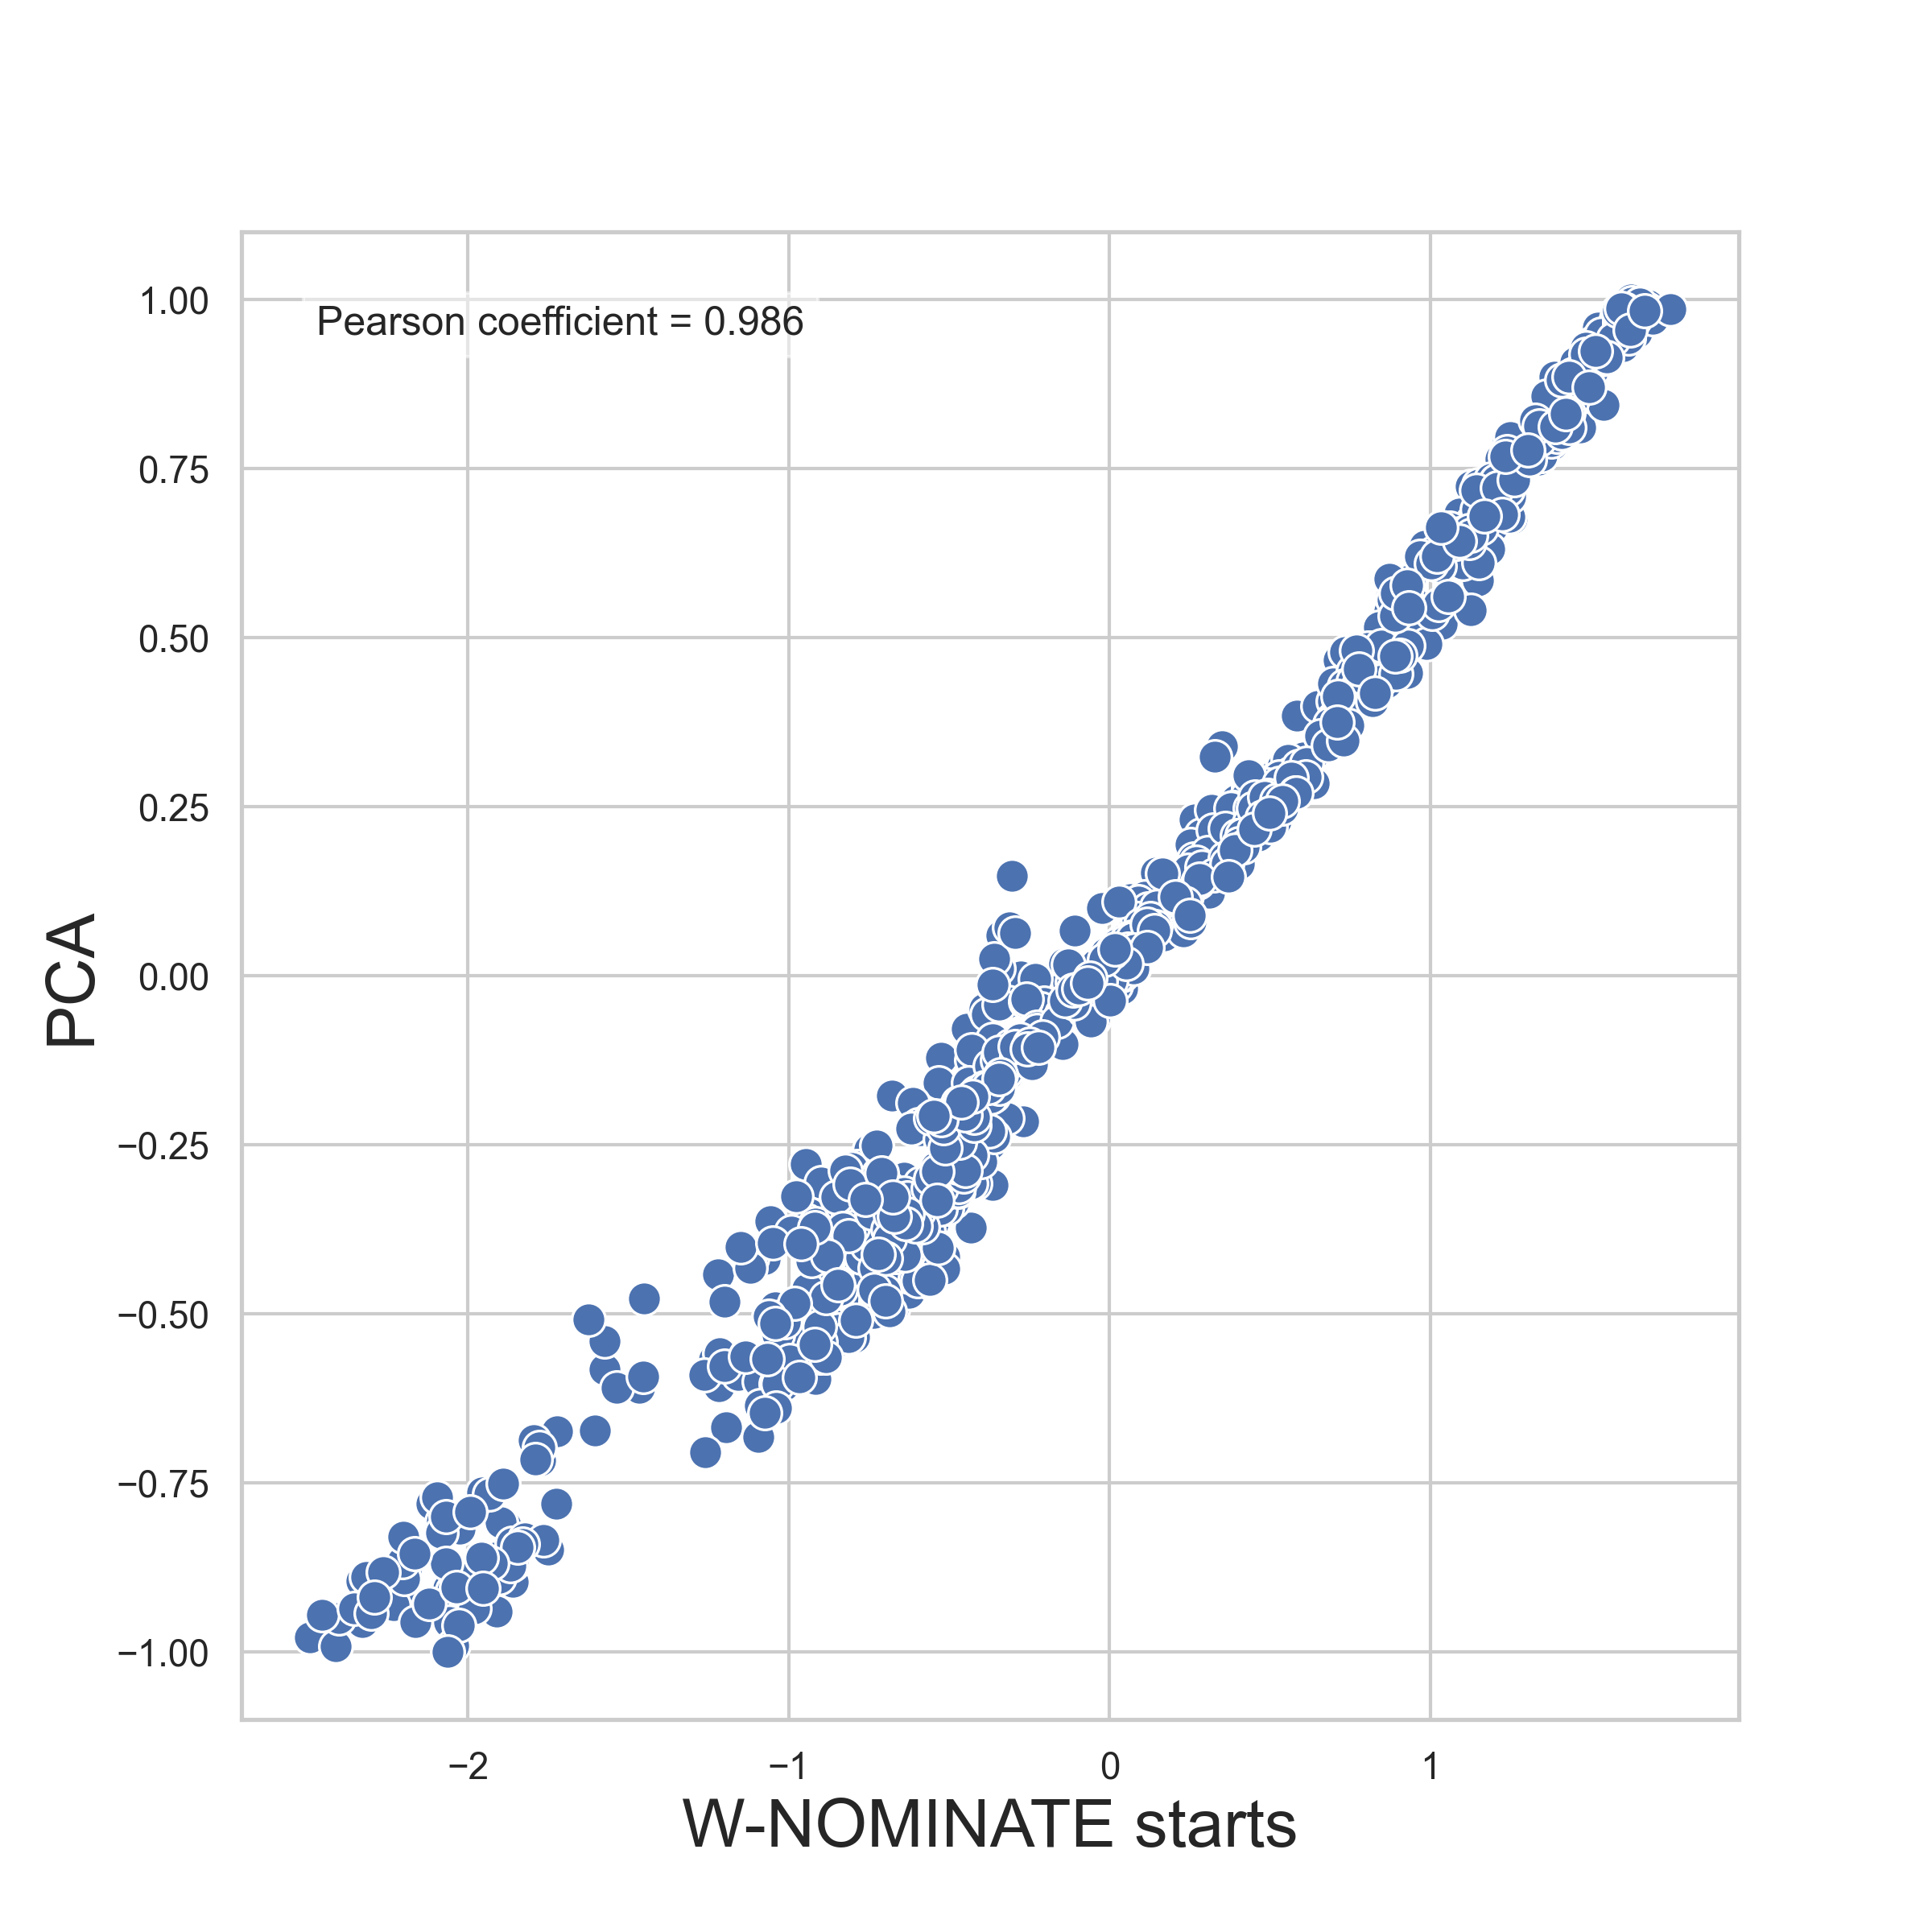
\includegraphics[width=\textwidth]{Graphs/Scatterstartspca6}
            \caption{PCA and W-NOMINATE starts in EP6}
            \label{fig:pca_SCATTER_6}
        \end{subfigure}
        \hfill
        \begin{subfigure}[b]{0.48\textwidth}
            \centering
            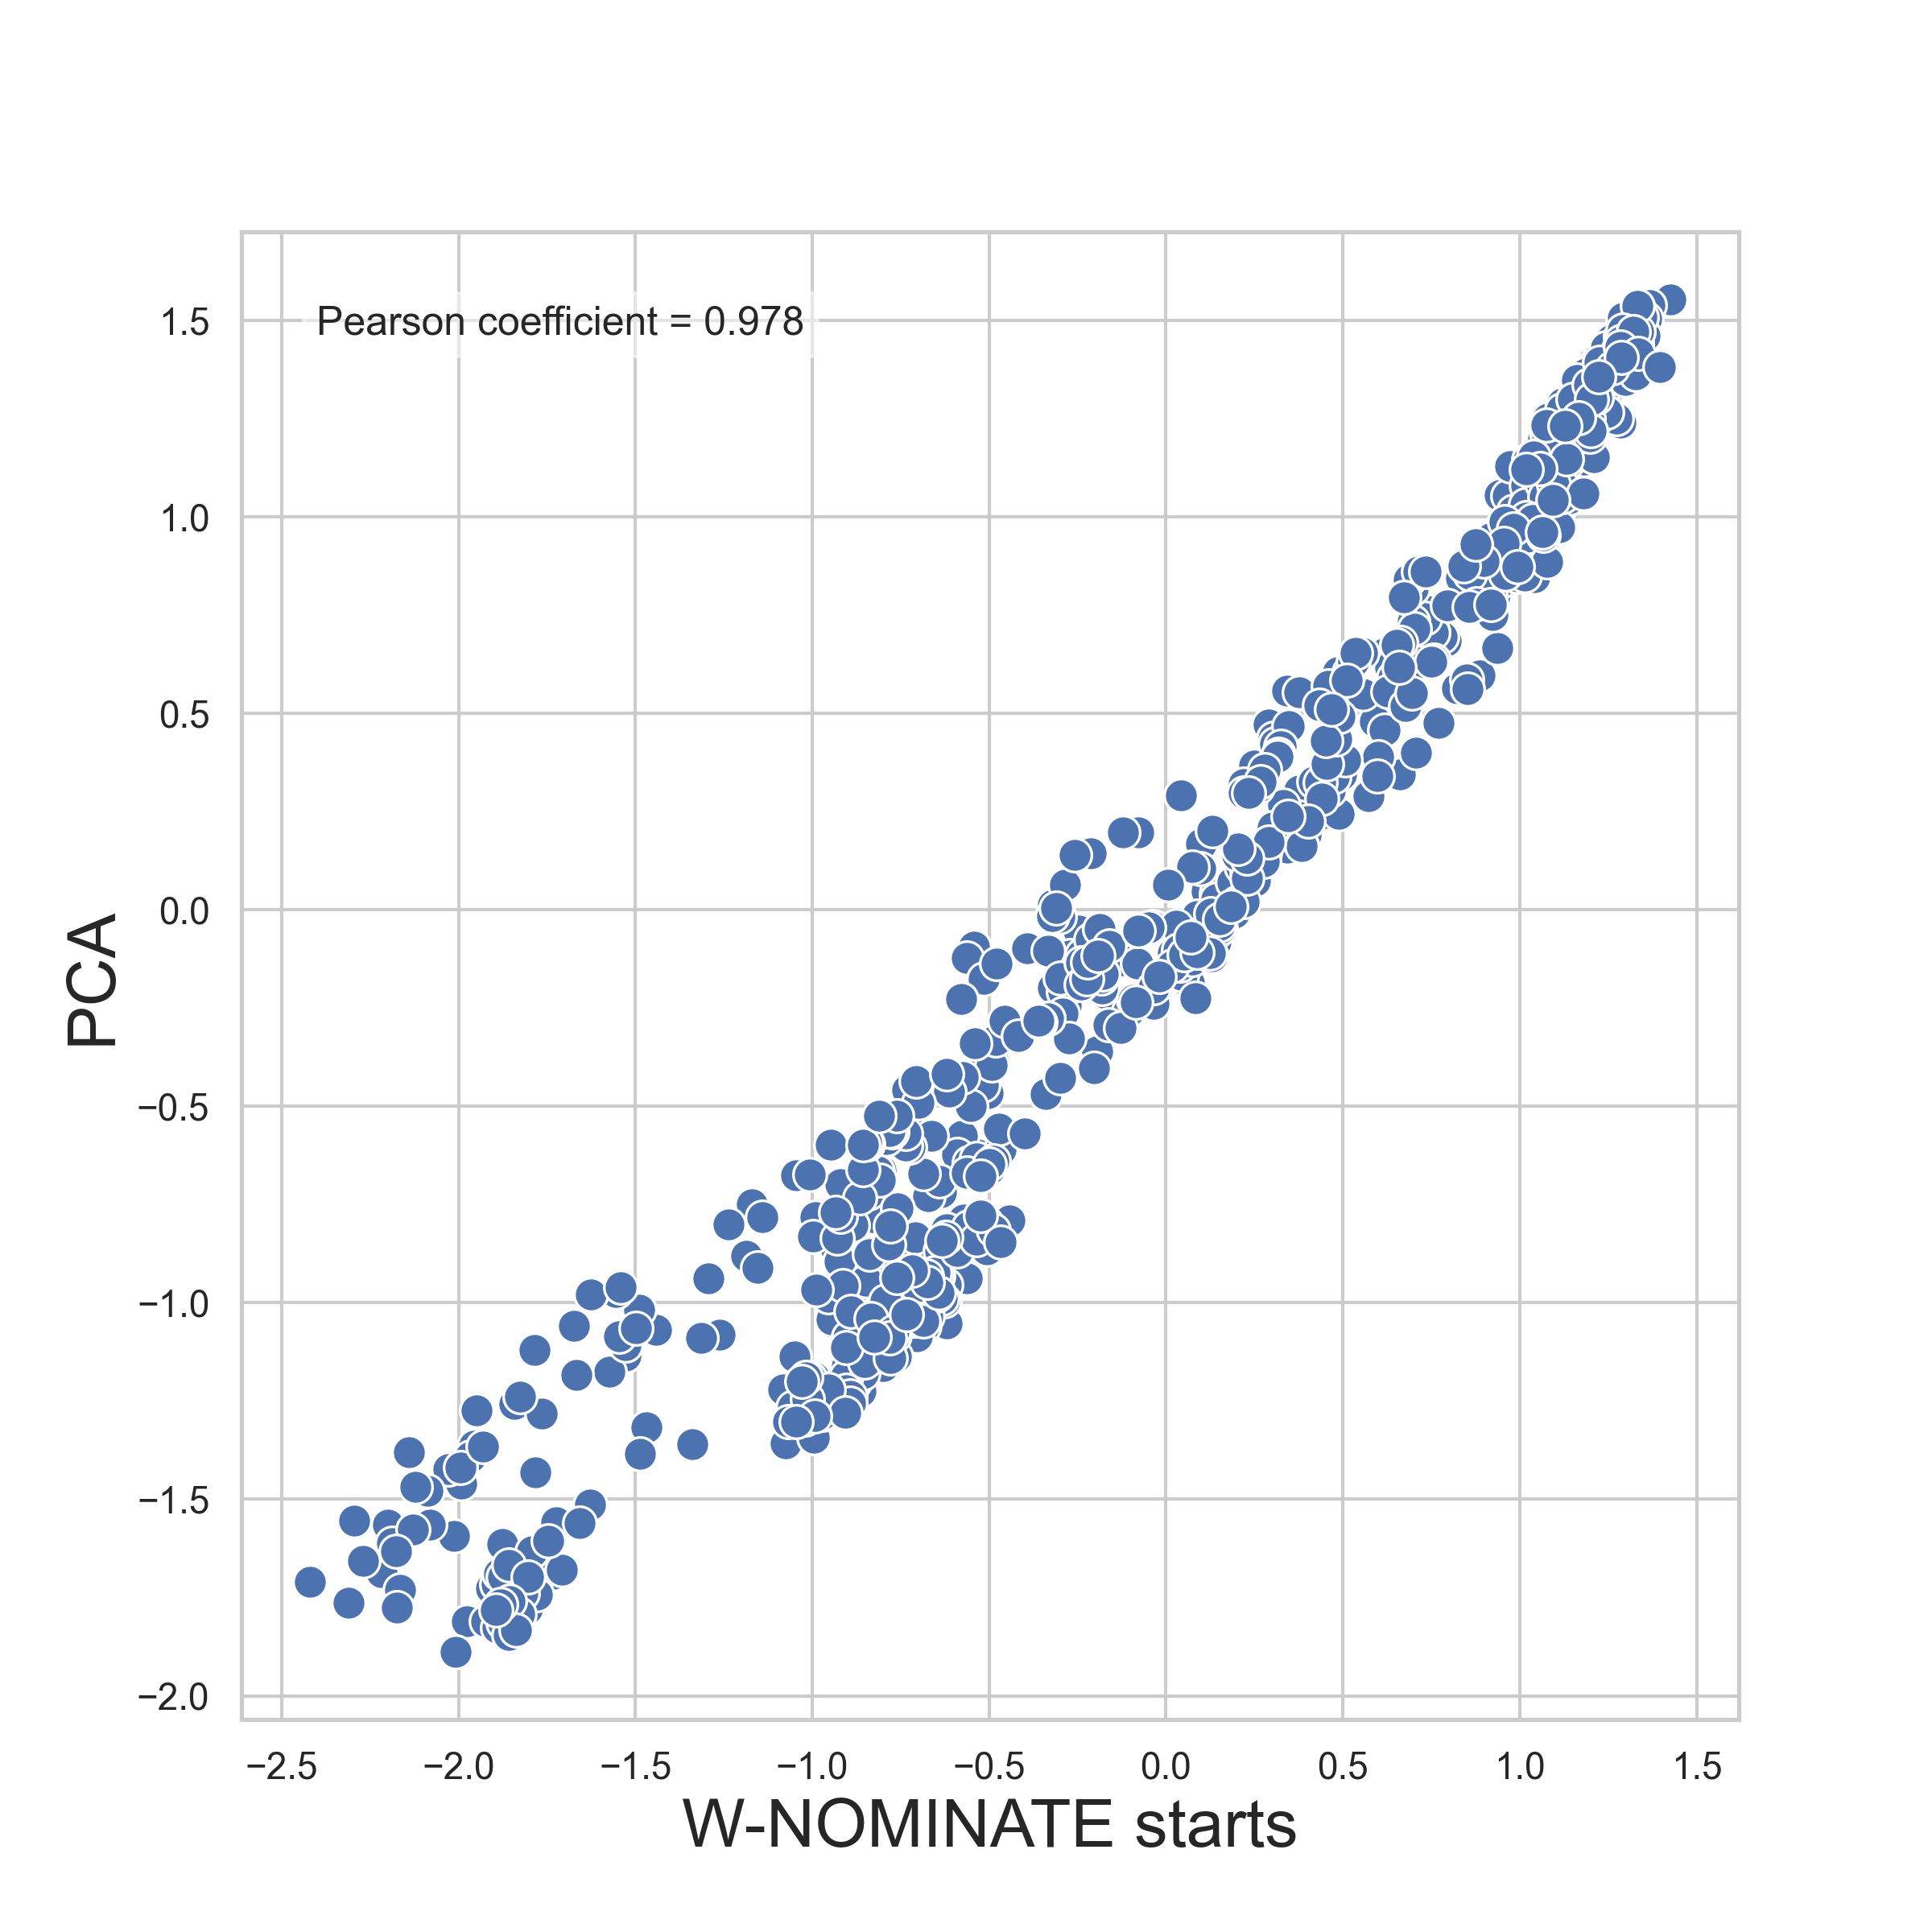
\includegraphics[width=\textwidth]{Graphs/Scatterstartspca7}
            \caption{PCA and W-NOMINATE starts in EP7}
            \label{fig:pca_SCATTER_7}
        \end{subfigure}
        \caption
        {Scatter plots of PCA and W-NOMINATE initialization scores in EP 6 and 7}
        \label{fig:pca_scatter67}
    \end{figure}
    \begin{figure}[H]
        \centering
        \begin{subfigure}[b]{0.48\textwidth}
            \centering
            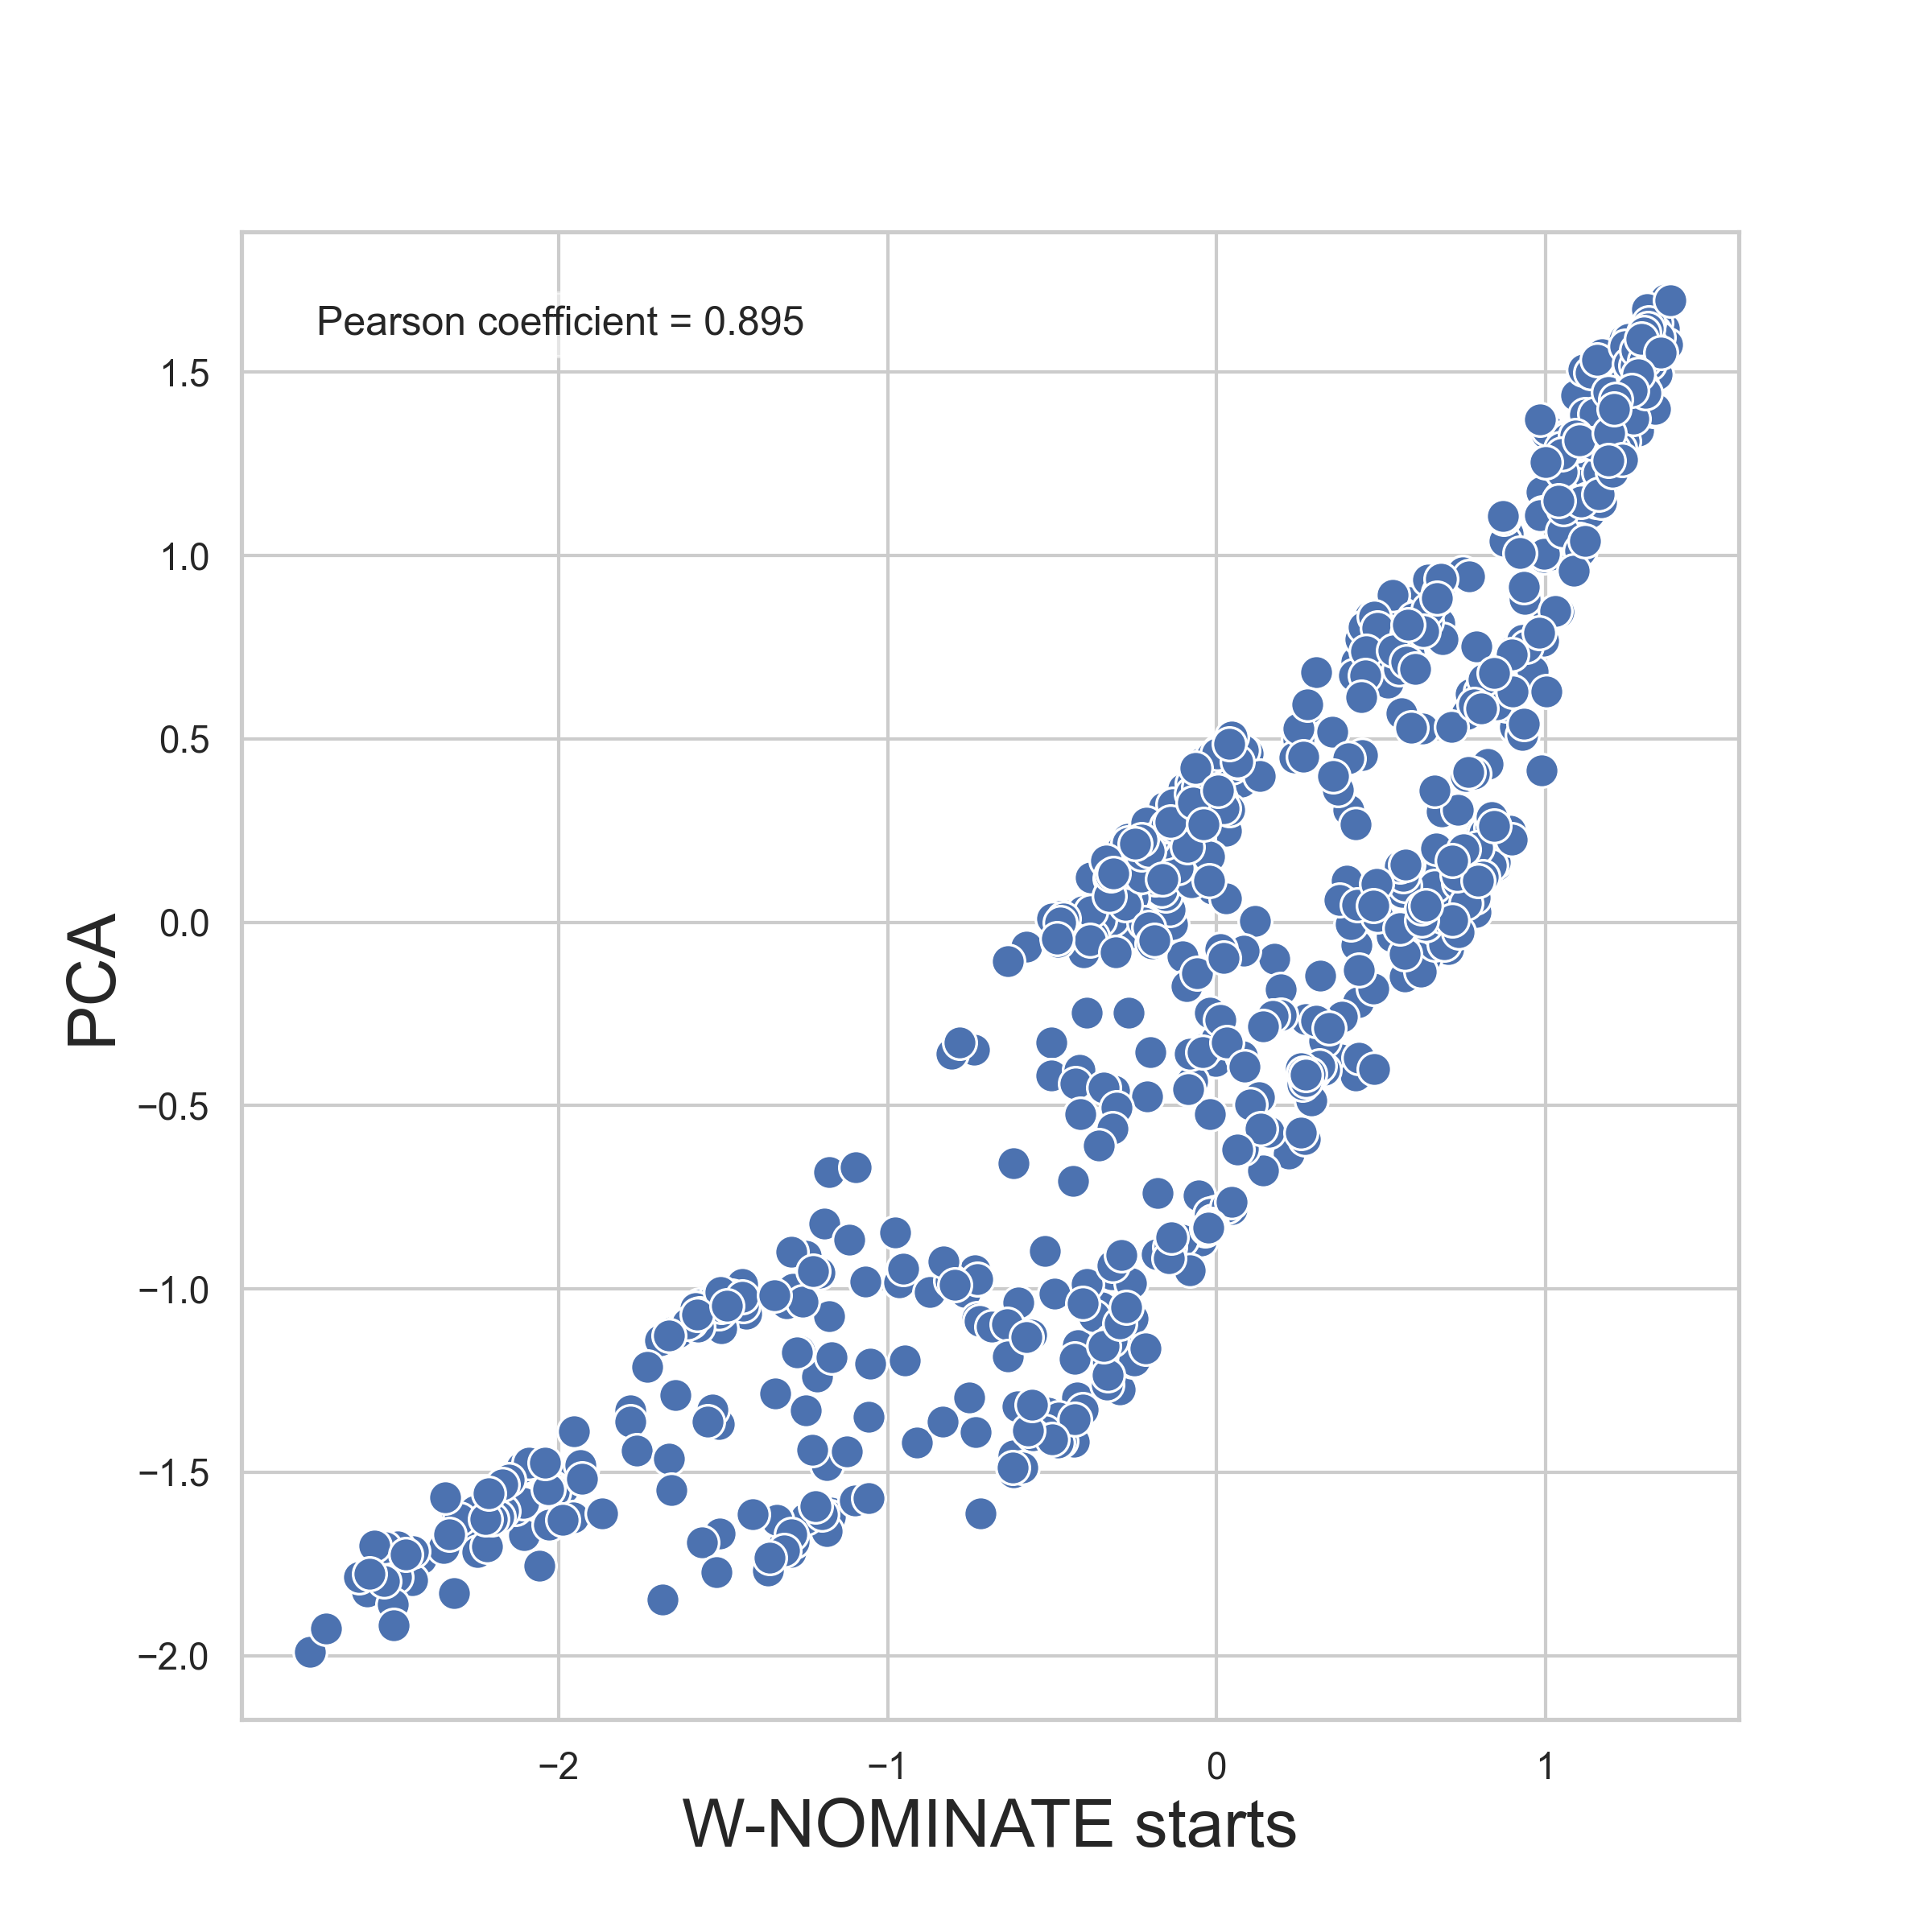
\includegraphics[width=\textwidth]{Graphs/Scatterstartspca8}
            \caption{PCA and W-NOMINATE starts in EP8}
            \label{fig:pca_SCATTER_8}
        \end{subfigure}
        \hfill
        \begin{subfigure}[b]{0.48\textwidth}
            \centering
            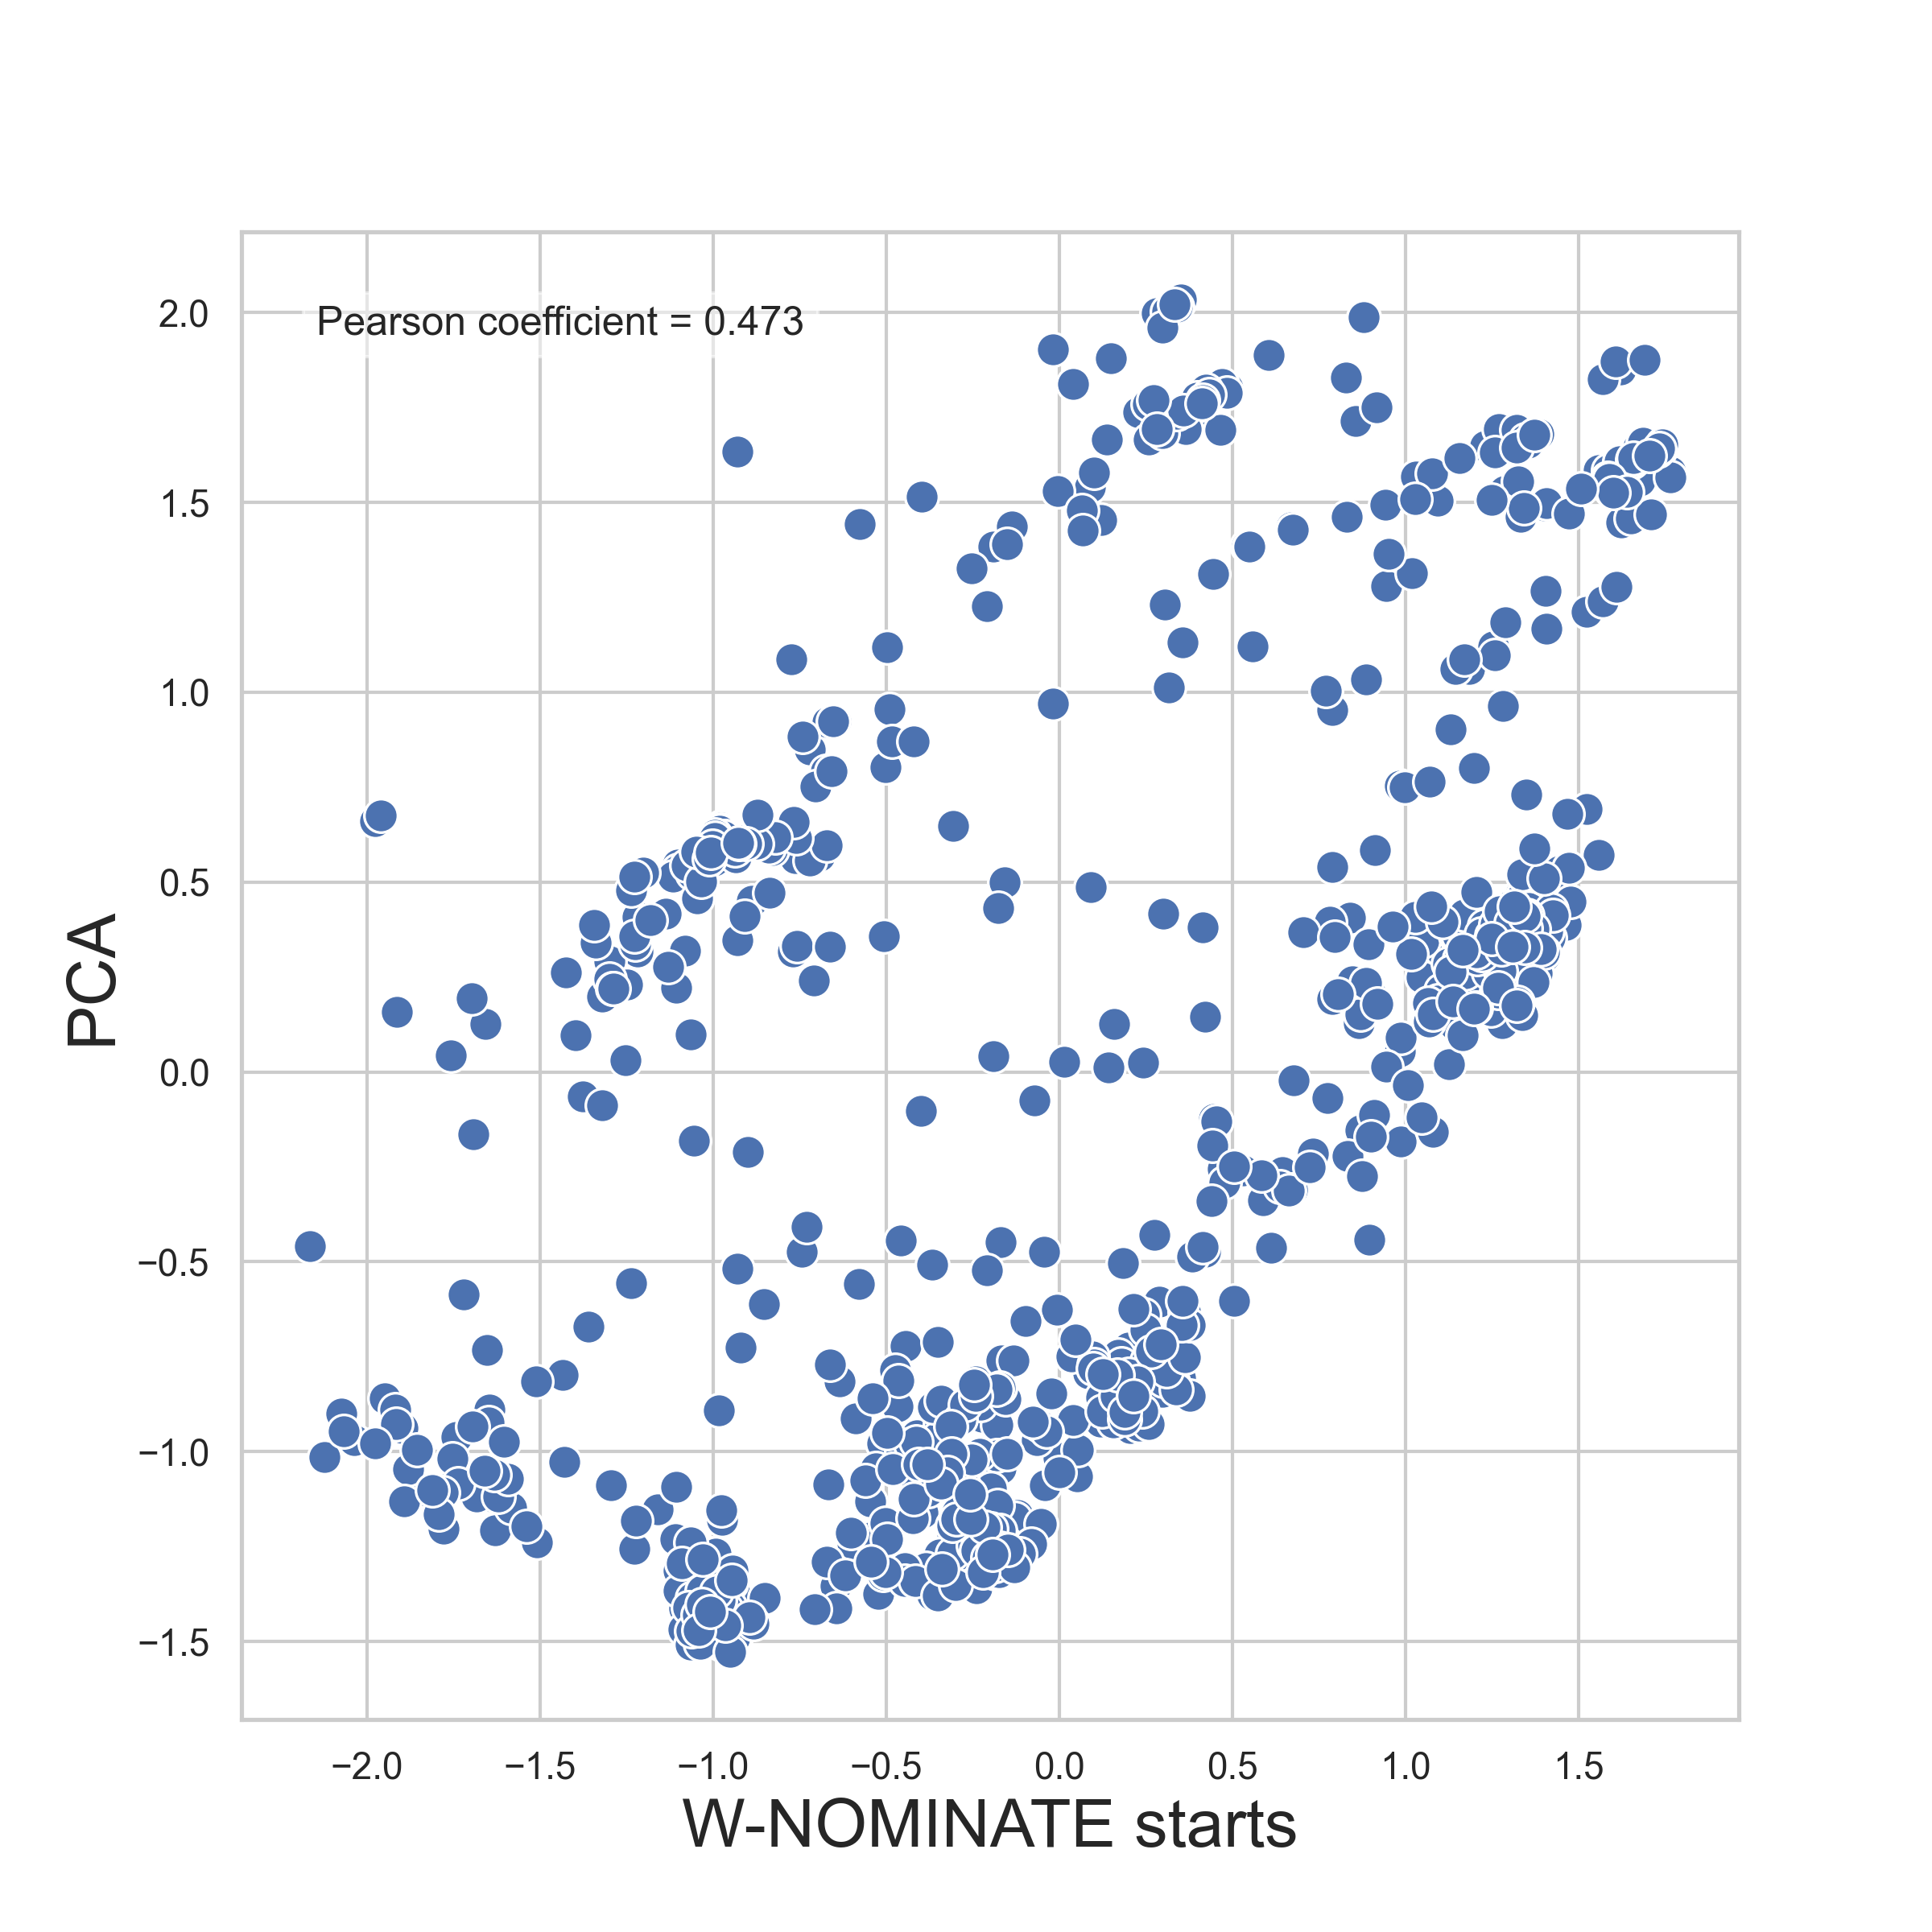
\includegraphics[width=\textwidth]{Graphs/Scatterstartspca9}
            \caption{PCA and W-NOMINATE starts in EP9}
            \label{fig:pca_SCATTER_9}
        \end{subfigure}
        \caption
        {Scatter plots of PCA and W-NOMINATE initialization scores in EP 8 and 9}
        \label{fig:pca_scatter89}
    \end{figure}


    \chapter{Analysing the structure of missing data}\label{ch:analysing-the-structure-of-missing-data}
    The datasets not only include detailed information on the votes cast by Members of the European Parliament (MEPs)
    but also account for instances of missing votes, such as when an MEP is absent during a vote. This data,
    combined with the data on MEPs enriched with demographic information, is an interesting starting point towards
    identifying the structure behind the missingness, or why and which MEPs are absent during votes.


    \section{Overview of missing data}\label{sec:overview-of-missing-data}

    \subsection{Types of missing data in the dataset}\label{subsec:types-of-missing-data-in-the-dataset}

    \begin{figure}[htb]
        \centering
        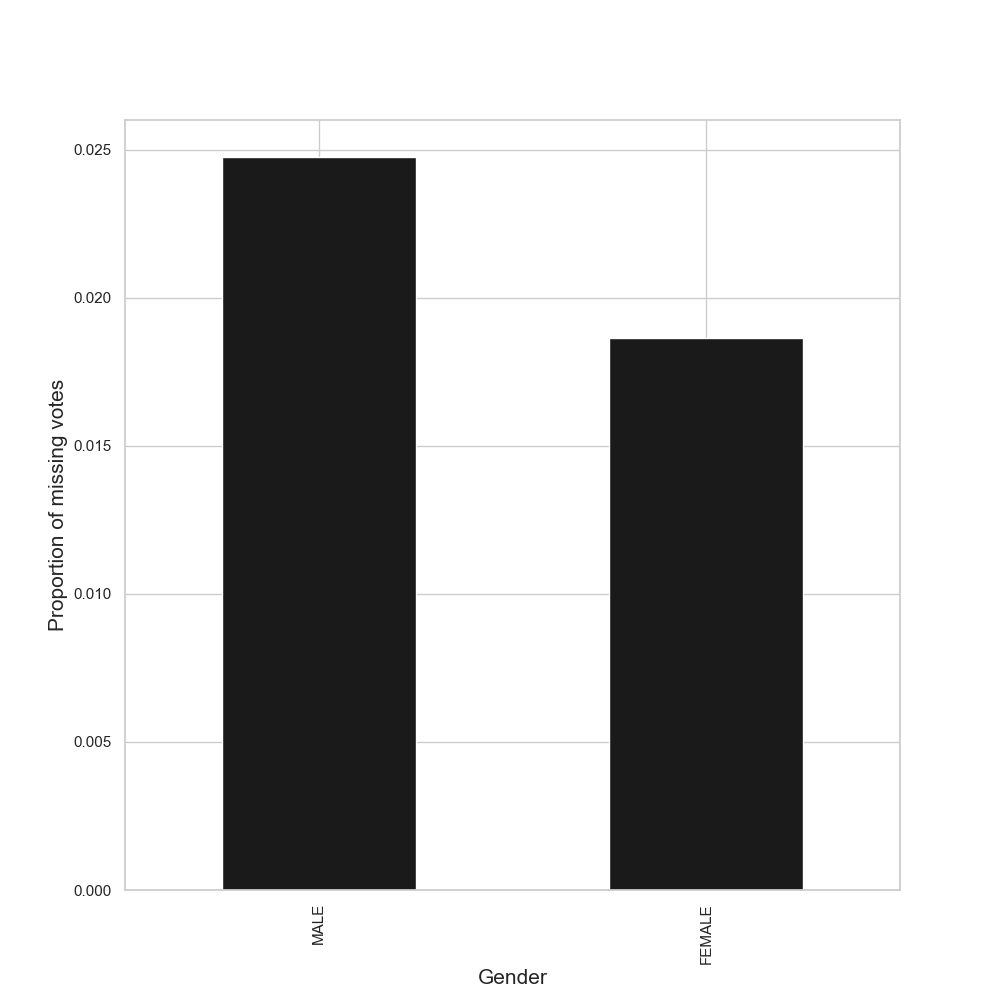
\includegraphics[width=0.65\textwidth]{Graphs/genderreport}
        \caption
        {Proportion of missing votes by Gender in EP 9. Male MEPs are more likely to be absent than female ones.}
        \label{fig:gender}
    \end{figure}

    \begin{figure}[htb]
        \centering
        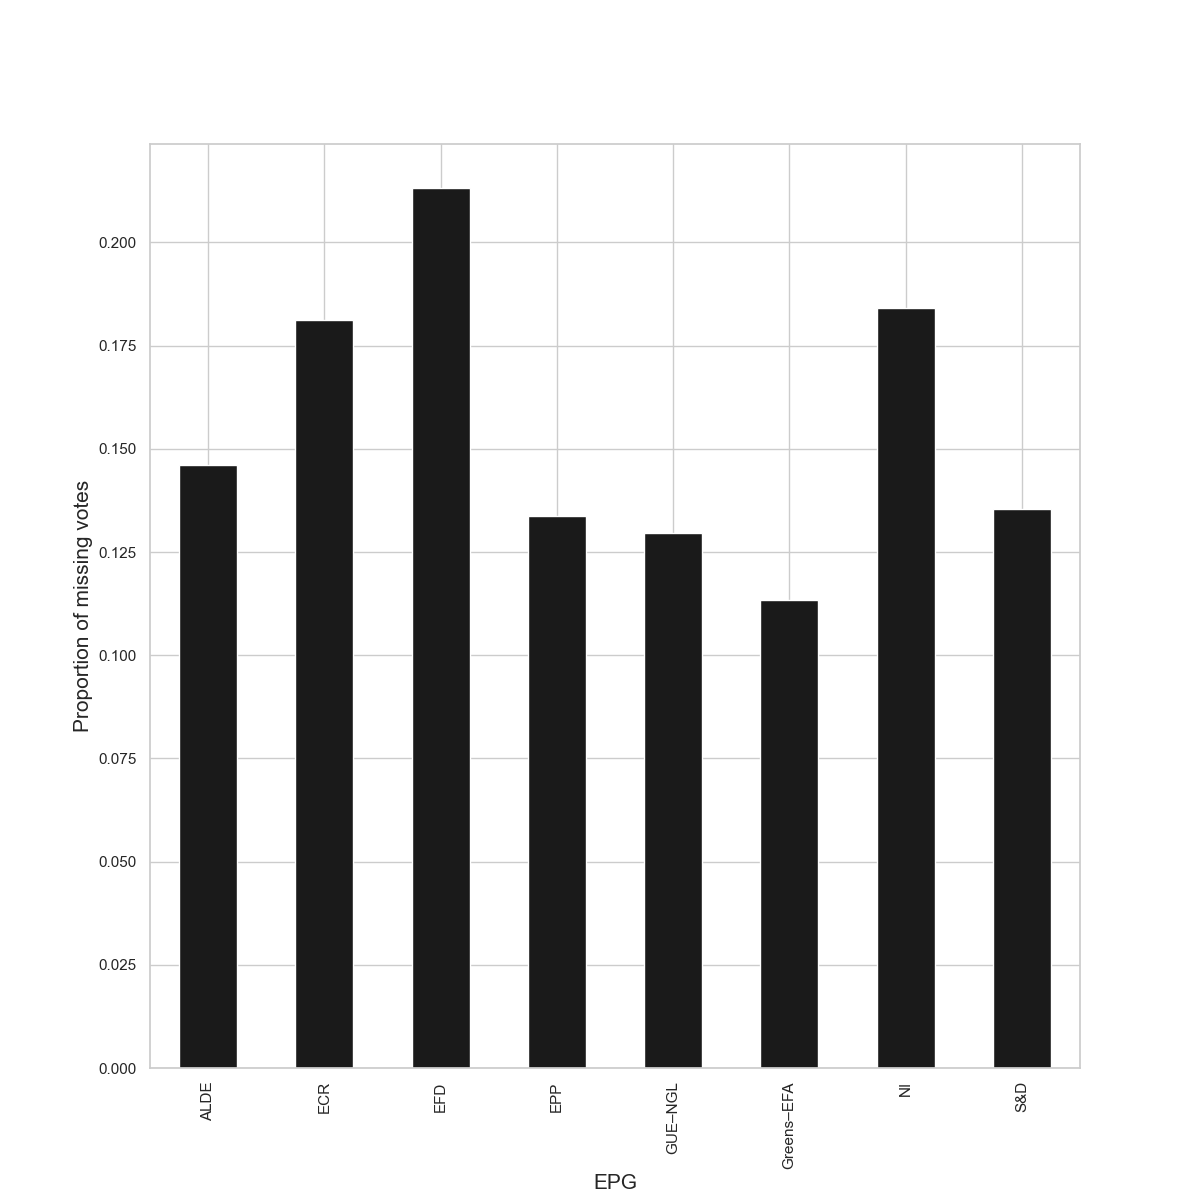
\includegraphics[width=0.65\textwidth]{Graphs/proportions_report}
        \caption{Proportion of missing votes by EPG in EP 7}
        \label{fig:proportions}
    \end{figure}

    \subsection{Describing the missingess}\label{subsec:describing-the-missingess}
    To explore this aspect of the data, we developed an interactive data visualization
    tool that categorizes and sorts the proportion of absences by various factors, including country of origin, gender,
    and European Political Group (EPG) affiliation. This initial implementation offers a basic yet
    informative view of
    absenteeism within the European Parliament, shedding light on how different demographic and political factors might
    correlate with voting attendance. As an example - male MEPs are consistently more absent than female MEPs (with
    exception of Parliament 8; See Figure~\ref{fig:gender}). Visualisation also gives an impression that eurosceptic
    or right-leaning parties tend to vote less often (See Figure~\ref{fig:proportions}).


    \section{Impact of ideology on missingness}\label{sec:impact-of-ideology-on-missingness}

    \subsection{Model}\label{subsec:model}

    \subsection{Results}\label{subsec:results}


    \chapter{Conclusions}\label{ch:conclusions}


\end{document}
